\documentclass[10pt]{article}
\usepackage[margin=0.8in,headheight=14pt]{geometry}
\usepackage{fontspec}\setmainfont{Arial}\setmonofont{Consolas}
\usepackage{amsmath,amssymb}
\usepackage{graphicx,booktabs,longtable,array,float,xcolor,caption,fancyhdr,tikz,enumitem}
\usetikzlibrary{arrows.meta,positioning,shapes.geometric}
\usepackage[hidelinks]{hyperref}
\definecolor{pass}{HTML}{1E7B3A}\definecolor{fail}{HTML}{B22222}\definecolor{warn}{HTML}{B0590B}
\definecolor{muted}{HTML}{5B6670}\definecolor{bp}{HTML}{1E5AA8}\definecolor{bpdeep}{HTML}{123A6E}
\captionsetup{font=small,labelfont=bf}
\setlength{\parskip}{0.5em}\setlength{\parindent}{0pt}
\setlist{nosep,leftmargin=1.4em}
\pagestyle{fancy}\fancyhf{}\lhead{\small RNGD AI Studio --- walkthrough and results}\rhead{\small\thepage}
\renewcommand{\headrulewidth}{0.4pt}
\renewcommand{\arraystretch}{1.12}
\begin{document}
\begin{titlepage}\centering
\vspace*{2cm}{\fontsize{40}{44}\selectfont\bfseries RNGD}\par\vspace{0.6cm}
{\LARGE Concept-to-Schematic AI Studio}\par\vspace{0.3cm}
{\Large System walkthrough and results}\par\vspace{1cm}
{\large A full run of every mode, with screenshots and the actual results of that run}\par\vspace{2cm}
\begin{tabular}{ll}Run & 2026-10-05 15:55:50 to 2026-10-05 16:01:56 \\
Report built & 2026-10-11 00:02 \\ App & \texttt{src/app.py} (Streamlit) \\\end{tabular}
\vfill{\small\color{fail} Semester proof of concept. Pipeline, IFC-studio zoning and BaaP data are synthetic; the
IFC file, IBC rule set, ADA standards and hotel program are RNGD-supplied. Not for construction.}
\end{titlepage}
\tableofcontents\newpage

\section{Executive summary}
This report documents a complete run of the RNGD AI Studio: every mode was driven through the real app in a
browser, the way a user would use it, and each screen was captured. The numbers below come from that run.
{\small \begin{longtable}{p{3.4cm}p{5.2cm}p{7.6cm}}
\toprule
\textbf{Mode} & \textbf{Headline result} & \textbf{Detail} \\ \midrule \endhead
Multi-Agent Pipeline & REVISE (93\%) & 2 conflicts; 11 agent steps \\
IFC Design Studio & 1/5 scenarios pass sample zoning & passing: Right-sized: 60 units, podium (compliant) \\
Open IFC File & IFC2X3, 1,537 elements & 3 storeys; 4 outliers excluded \\
Hotel Schematic & 117 keys, 6 levels & 13/16 checks pass; fails: Stories above grade \\
Layout optimization & 192 rooms placed on the 3 QA sites, 0 without a window & reference GA: 171 rooms, 24 without a window; hotel: 740 layouts in 36 s, first choice Bar 265x58 · center core \\
Automated tests & 51/51 pass &  \\
\bottomrule
\end{longtable}}
\textbf{Key findings}
\begin{itemize}
\item \textbf{Pipeline:} (see the data-source note in the pipeline section) the arbiter returned \textbf{REVISE}. The building footprint itself is geometrically compliant (no setback, easement, or overlap violations; lot coverage 46.3\%), but the design fails to resolve a critical, high-severity parking conflict identified earlier in the pipeline. The site plan delivers only 15 surface parking stalls against a required 150 (1.25/unit), a shortfall of 135 stalls. The critic loop explicitly acknowledged this cannot be fixed by mino...
\item \textbf{IFC Design Studio:} the Baseline (120 units) fails 4 sample-zoning check(s): FAR, Lot coverage \%, Parking stalls, Building inside setbacks/easement. Scenarios passing all sample checks: Right-sized: 60 units, podium (compliant). Against RNGD's real IBC rules the Right-sized scenario still fails: IBC-R1-027 (Dead-end corridor maximum for sprinklered R-1).
\item \textbf{Real IFC file:} opened and summarised without errors; far-away outliers are excluded so the building fills the view.
\item \textbf{Hotel:} 117 of 117 keys placed on 5 guest floors; failing checks: Stories above grade (a Type IA podium or one fewer guest floor resolves the story limit). ADA mobility rooms: 7 provided vs $\ge$ 7 for 117 rooms (5 + 2 with roll-in) (PASS).
\item \textbf{Layout optimization (Section~\ref{sec:opt}):} on the three QA sites the updated optimizer places 192 rooms with 0 windowless guest rooms in 59 s, against 171 rooms with 24 windowless for the reference GA (same program, same evaluator). In Hotel Schematic it generated and ranked 740 layouts in 36 s; the first-ranked one (Bar 265x58 · center core, 4 guest floors) places 117 of 117 keys. No language model is used in the optimization.
\item \textbf{Quality:} 0 on-page errors during the browser run; 51 of 51 automated tests passed.
\end{itemize}

\section{How the run was done}
\begin{enumerate}
\item The app was started with \texttt{streamlit run src/app.py} on \texttt{localhost:8501}.
\item \texttt{src/capture\_app.py} drove headless Chrome through every mode: ran the full pipeline, generated the
Baseline and Right-sized IFC scenarios, opened the real IFC file, used every tab of the hotel workspace, generated the
hotel PDF, and asked the assistant a question. It waited for each step to finish before taking a screenshot.
\item This report reads the results those steps saved (\texttt{outputs/project\_001/project\_state.json}, the hotel
report manifest), recomputes the deterministic results (IFC scenarios, hotel schematic) and runs the test suite.
\end{enumerate}
{\small \begin{longtable}{p{5cm}p{11cm}}
\toprule
\textbf{Setting} & \textbf{Value} \\ \midrule \endhead
Run date & 2026-10-05 15:55:50 \\
Python / Streamlit & 3.11.11 / 1.52.2 \\
OS & Windows 10 \\
LLM provider & OpenRouter (Chinese-developed models are blocked in code) \\
Light model & openai/gpt-oss-20b \\
Reasoning model & openai/gpt-oss-120b \\
Arbiter model & anthropic/claude-sonnet-5 \\
Report-writer model & anthropic/claude-sonnet-5.5 \\
Embeddings & all-MiniLM-L6-v2 \\
Screenshots & 31 at 1680 x 1050 px, headless Chrome \\
On-page errors during the run & 0 \\
\bottomrule
\end{longtable}}
{\small \begin{longtable}{p{6cm}p{3cm}}
\toprule
\textbf{Step} & \textbf{Time} \\ \midrule \endhead
startup & 2.2 s \\
pipeline run & 104.8 s \\
ifc baseline & 3.8 s \\
ifc rightsized & 5.1 s \\
ifc open & 52.4 s \\
hotel pdf & 24.2 s \\
assistant reply & 36.8 s \\
\bottomrule
\end{longtable}}

\section{System architecture}
Section~\ref{sec:methods} explains how each design is generated and which technology is used.
\begin{figure}[H]\centering
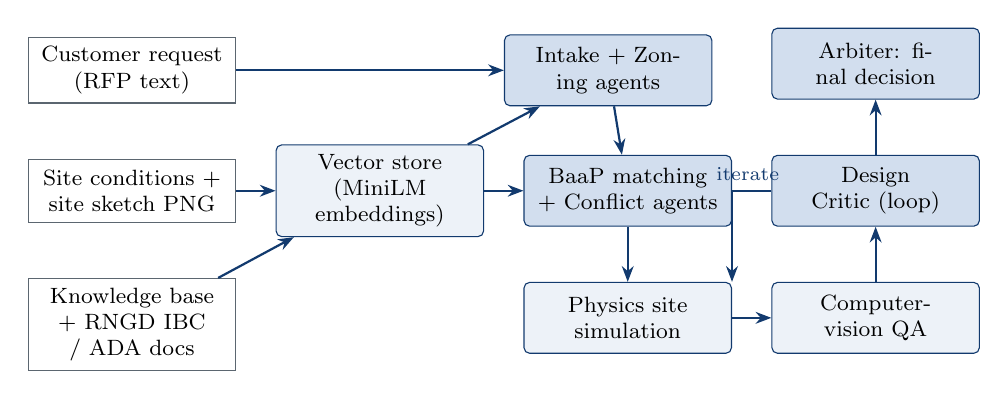
\begin{tikzpicture}[node distance=7mm and 5mm, every node/.style={font=\footnotesize},
 box/.style={draw=bpdeep, fill=bp!8, rounded corners=2pt, align=center, minimum height=9mm, text width=24mm},
 data/.style={draw=muted, fill=white, align=center, minimum height=8mm, text width=24mm},
 ai/.style={box, fill=bp!20}, arr/.style={-{Stealth[length=2mm]}, thick, bpdeep}]
\node[data] (rfp) {Customer request (RFP text)};
\node[data, below=of rfp] (site) {Site conditions + site sketch PNG};
\node[data, below=of site] (docs) {Knowledge base + RNGD IBC / ADA docs};
\node[box, right=of site] (vec) {Vector store (MiniLM embeddings)};
\node[ai, right=of rfp, xshift=29mm] (intake) {Intake + Zoning agents};
\node[ai, right=of vec] (baap) {BaaP matching + Conflict agents};
\node[box, below=of baap] (sim) {Physics site simulation};
\node[box, right=of sim] (cv) {Computer-vision QA};
\node[ai, above=of cv] (crit) {Design Critic (loop)};
\node[ai, above=of crit] (arb) {Arbiter: final decision};
\draw[arr] (rfp) -- (intake); \draw[arr] (site) -- (vec); \draw[arr] (docs) -- (vec);
\draw[arr] (vec) -- (intake); \draw[arr] (vec) -- (baap); \draw[arr] (intake) -- (baap);
\draw[arr] (baap) -- (sim); \draw[arr] (sim) -- (cv); \draw[arr] (cv) -- (crit);
\draw[arr] (crit.west) -| node[above, pos=0.3]{\scriptsize iterate} (sim.north east); \draw[arr] (crit) -- (arb);
\end{tikzpicture}
\caption{Multi-agent pipeline. Shaded boxes call an LLM through OpenRouter; the others are deterministic Python.}
\end{figure}
\begin{figure}[H]\centering
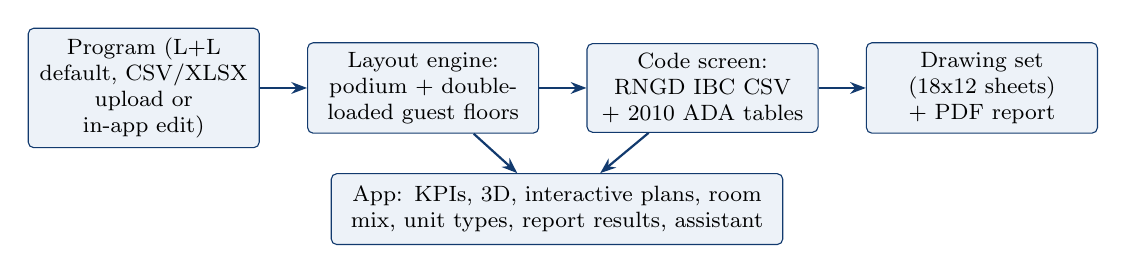
\begin{tikzpicture}[node distance=5mm and 6mm, every node/.style={font=\footnotesize},
 box/.style={draw=bpdeep, fill=bp!8, rounded corners=2pt, align=center, minimum height=9mm, text width=27mm},
 arr/.style={-{Stealth[length=2mm]}, thick, bpdeep}]
\node[box] (p) {Program (L+L default, CSV/XLSX upload or in-app edit)};
\node[box, right=of p] (l) {Layout engine: podium + double-loaded guest floors};
\node[box, right=of l] (c) {Code screen: RNGD IBC CSV + 2010 ADA tables};
\node[box, right=of c] (d) {Drawing set (18x12 sheets) + PDF report};
\node[box, below=of l, text width=55mm, xshift=17mm] (ui) {App: KPIs, 3D, interactive plans, room mix, unit types, report results, assistant};
\draw[arr] (p) -- (l); \draw[arr] (l) -- (c); \draw[arr] (c) -- (d); \draw[arr] (l) -- (ui); \draw[arr] (c) -- (ui);
\end{tikzpicture}
\caption{Hotel Schematic mode (RNGD's first use case): deterministic, no LLM needed except the assistant.}
\end{figure}


\section{How the designs were created: methods and technology}
\label{sec:methods}
Every design in this report is produced by code in this repository. Only the agent steps of the pipeline and the chat
assistant use a language model; all geometry (site plans, floor plates, IFC models, hotel plans, drawing sheets and
3D views) is computed deterministically, so the same inputs always give the same design.

\subsection{Technology stack}
{\small
\begin{longtable}{p{3.6cm}p{4.4cm}p{8cm}}\toprule
\textbf{Layer} & \textbf{Technology} & \textbf{Used for} \\ \midrule \endhead
Language & Python 3.11 & All engines, agents, drawings and report builders. \\
User interface & Streamlit 1.52 & The five-mode web app, chat panel, program editor and report downloads. \\
Language models & OpenRouter (OpenAI-compatible SDK) & Agent steps and the assistant. A light model for parsing, a reasoning model for analysis, a Claude model for the single arbiter call. Chinese-developed models are blocked in code; requests time out after 90 s. \\
Retrieval (RAG) & sentence-transformers all-MiniLM-L6-v2 (TF-IDF fallback) & Vector store over the sample knowledge base plus RNGD's real IBC rule CSV / workbook and the ADA 2010 PDF, tagged synthetic vs real. \\
Shared state & pydantic models (\texttt{ProjectState}) & A blackboard every pipeline agent reads and writes, with a full trace of each step. \\
Layout optimization & NumPy, SciPy ndimage, scikit-image (least-cost paths), process pool & Architectural decoder, ten-objective fitness, systematic search and memetic GA, plate generator, Pareto + TOPSIS decision (Section~\ref{sec:opt}). No language model in the loop. \\
Physics simulation & NumPy / SciPy & 2D rigid-body relaxation that places the building, driveway and parking inside the buildable envelope. \\
Computer vision & SciPy ndimage, scikit-image & Reads the site sketch and re-measures the rendered site plan (setbacks, easement, overlaps, parking stalls). \\
BIM / IFC & IfcOpenShell & Writes IFC4 models (IFC Design Studio) and reads / triangulates real IFC2X3 files (Open IFC File). \\
Data inputs & pandas, openpyxl, PyMuPDF & Program CSV/XLSX upload, RNGD's IBC rule CSV and workbook, text of the ADA PDF. \\
Interactive graphics & Plotly & 3D models (Mesh3d) and hoverable floor plans in the app. \\
Drawings & Matplotlib (vector PDF + PNG) & Site plans, floor plates, the 18 x 12 in hotel drawing sheets and the isometric unit / building views. \\
Documents & LaTeX via Tectonic (XeTeX), PyMuPDF & PDF reports, merged with the drawing sheets. \\
Verification & pytest, Streamlit AppTest, Playwright + Chrome & Automated tests and the browser run that produced the screenshots in this report. \\
\bottomrule\end{longtable}}

\subsection{Multi-agent pipeline (concept to schematic)}
\begin{enumerate}
\item \textbf{Inputs.} A free-text customer request, \texttt{site\_conditions.json} and a site sketch PNG with a georeference file.
\item \textbf{Vision input (classical CV).} The sketch is thresholded and its lot outline and easement measured in feet using the georeference, then cross-checked against the stated site conditions.
\item \textbf{Intake agent (LLM).} Turns the request into a structured program: unit count and mix, floors, amenities, parking preference, budget, hard vs soft requirements. The model must return JSON; malformed JSON is sent back for correction.
\item \textbf{Zoning agent (LLM + RAG).} Retrieves the applicable zoning passages and extracts limits (height, stories, FAR, coverage, parking ratio, setbacks). The buildable envelope is then computed in plain Python, not by the model.
\item \textbf{BaaP matching agent (LLM + RAG).} Converts the unit mix into exact module counts from the BaaP catalog and estimates gross area and footprint per floor.
\item \textbf{Conflict agent (LLM).} Computes feasibility numbers (FAR, coverage, parking demand vs land) and lists conflicts with severities and recommendations.
\item \textbf{Physics simulation.} Building, driveway and parking blocks are rigid bodies with containment forces (stay inside the envelope) and separation forces (no overlaps); the system is relaxed until the overlap penalty converges, then rendered as a site plan.
\item \textbf{Vision QA.} The rendered plan image is re-measured independently at a known DPI to count stalls and detect setback, easement and overlap violations.
\item \textbf{Design critic (LLM) and loop.} Decides whether another simulation pass with adjusted parameters can fix a violation, or whether it is a program / site conflict no geometry change can solve (up to the configured number of iterations).
\item \textbf{Floor plate packer (rules).} Lays unit modules along a double-loaded corridor for a ground and a typical floor.
\item \textbf{Arbiter (one Claude call).} Reads the whole blackboard and returns APPROVE, APPROVE WITH CONDITIONS, REVISE or INSUFFICIENT INFORMATION with a narrative, unresolved issues and next steps.
\end{enumerate}

\subsection{IFC Design Studio (parametric IFC4 model)}
\begin{enumerate}
\item \textbf{Parameters.} Lot, east easement, zoning preset, unit count and mix, floors, wings, parking type (surface or podium), corridor width and floor heights. Five preset scenarios fill these in.
\item \textbf{Modules.} The unit mix is turned into module counts from the shared BaaP catalog (\texttt{data/baap\_catalog.json}), including accessible units, a core, lobby, fitness and BOH/loading.
\item \textbf{Layout.} Units are placed on double-loaded corridor wings inside the setbacks and easement. The generator tries one to three wings and keeps the best by score: all units placed, building inside the envelope, a fire lane present, fewest wings.
\item \textbf{Parking.} Surface parking is found by scanning the free part of the lot for stall rows; podium parking places stalls under the building as well.
\item \textbf{Checks.} Ten sample-zoning checks (units, stories, height, FAR, coverage, parking, setbacks/easement, fire lane, accessible units, exit travel), plus a cross-check of measurable rules from RNGD's real IBC CSV (height, stories, exit travel, dead-end corridor, exits per story).
\item \textbf{IFC output.} IfcOpenShell writes a standard IFC4 file with project, site, building and one storey per level, and the unit, core and amenity volumes and slabs on each storey. The file opens in any BIM tool; the app re-reads it for the 3D viewer.
\end{enumerate}

\subsection{Open IFC File (real model viewer)}
\begin{enumerate}
\item IfcOpenShell reads the file's header, project, site, building, storeys and element counts by class.
\item Its geometry iterator triangulates each element (fine curtain-wall framing can be skipped for speed); the meshes are merged per class with NumPy and cached so a second open is fast.
\item The model is recentred on the median of its structural elements; elements more than four building-diagonals (at least 50 m) away are dropped from the view and listed, which is why the real model fills the screen. The original file is never modified.
\end{enumerate}

\subsection{Hotel Schematic (RNGD's first use case)}
\begin{enumerate}
\item \textbf{Program.} Default: the Project Renegade Living + Lodging cover-sheet space allocation, row for row (28 rows, 117 keys, 59,350 SF). A CSV/XLSX upload or the in-app editor can replace it; area is the total for each row, and the category (guest, shared, BOH, business, tenant) is read or inferred from the name.
\item \textbf{Sorting the program.} Guest rows become keys. Small repeated rooms (Ice, IT, Jan, Supplies) are placed once on every guest floor; small single BOH rooms go into the Level 1 core zone; tenant space becomes a retail block; stairs and corridors are generated, not packed.
\item \textbf{Guest floors.} Double-loaded corridor, 6 ft clear; room depth 26 ft and room width = program area / 26 ft. Keys are spread evenly over the floors, largest units first, and alternately to the south and north sides so both ends line up. A 34 ft core at the west end holds Stair 1, two elevators and shafts; Stair 2 is at the east end, so the corridor has an exit at each end. Alternate rooms are mirrored so bathrooms pair up.
\item \textbf{Level 1.} The same core stacked below; the lobby first on the street side, other rooms balanced between the two sides; the retail block full depth at the east end, wrapping Stair 2 so stairs stack on every level.
\item \textbf{Massing and areas.} Floor-to-floor heights come from the L+L elevations (Level 2 at 16 ft, then 10.75 ft); gross area is drawn length times width per level and is compared with the source sheets and with the meeting rule (33\% circulation, 8\% wall burden, rounded up to 100 SF).
\item \textbf{Code screen.} Rules from RNGD's IBC CSV are evaluated from the geometry: stories, height, area per story, high-rise screen, exits, exit separation (1/3 diagonal), travel distance, corridor width, dead-end corridor and door width, with occupant loads from the CSV's factors. ADA 2010 Tables 224.2, 224.4 and 224.5 set the accessible-room counts. Each failing item gets a suggested fix.
\item \textbf{Room detailing.} Each room type is described once in local coordinates (walls with door openings, door swings, bathroom fixtures, beds sized by type, closet, desk, suite partition, spa tub, ADA turning circles) and then transformed into every room on every plan, so plans, enlarged plans and 3D views always agree.
\item \textbf{Drawing sheets.} Matplotlib draws vector sheets at true scale in the RNGD L+L format: title block, colour-coded zones, column grid at 30--34 ft bays with bubbles, dimension strings, elevations with an indicative prefab panel breakdown, schedules (gross area, room count, space allocation), enlarged plans and unit 3D views.
\item \textbf{3D views.} In the app, Plotly Mesh3d draws every room as a coloured block (hover for details). On the sheets, a small orthographic projector draws boxes with back-face culling and depth sorting (a painter's algorithm), shading faces by orientation; OpenGL was not used.
\item \textbf{Report.} LaTeX (Tectonic) builds the front matter and appendices; PyMuPDF merges them with the sheets; a JSON manifest records the results so the app's report tab shows them later.
\end{enumerate}

\subsection{Layout optimization (Hotel Schematic ``Optimize layouts'' and Design Optimizer)}
Section~\ref{sec:opt} gives the architecture, the mathematics and the measured comparison with the reference genetic
algorithm. In short: a decoder turns a short genome into a valid plan (straight corridor spines one room depth from the
facade, modular bays, rooms assigned to bays), a deterministic fitness scores it, and a systematic search with pattern-search
refinement (or a GA) drives the genome. In Hotel Schematic the building shape, the core and stair positions and the floor
count are generated as well, and a multi-criteria decision step ranks every distinct layout.

\subsection{How this report was made}
\texttt{src/capture\_app.py} drives the running app in headless Chrome with Playwright, waits for each step to finish, takes the
screenshots and records timings, on-page errors and the assistant's replies. \texttt{src/build\_walkthrough\_report.py}
reads those results, recomputes the deterministic ones, runs or reuses the pytest results and compiles this PDF.
\texttt{src/build\_optimizer\_study.py} runs the optimization comparison (reference GA against the updated optimizer, and the
hotel layout exploration) and saves its numbers and figures for Section~\ref{sec:opt}.


\section{Multi-agent pipeline (project\_001, Elm Street Multifamily --- sample data)}
\subsection{What it does}
The pipeline turns an unstructured customer request and the site conditions into a Building-as-a-Product (BaaP)
schematic: agents parse the program and zoning, match BaaP modules, find conflicts, a physics-style solver places the
building and parking, computer vision re-measures the rendered plan, a critic decides whether to iterate, and one
arbiter call makes the final decision. The inputs are synthetic sample data.

\textbf{Customer request (excerpt):}\par
\begin{quote}\small Subject: Elm Street Multifamily — Program for Concept Design

We'd like RNGD to develop a concept-to-schematic design for our Elm Street site
(200 ft of frontage on Elm Street, 300 ft deep, zoned R-4). We are targeting a
4-story, 120-unit market-rate multifamily community.

Unit mix: roughly 20\% studios, 45\% one-bedrooms, and 35\% two-bedrooms. 120 total
units is a firm, hard requirement from our lender — please do not go below it, though
we could go slightly over if the site allows.

Amenities we need: a resident fitness room, a lobby with an integrated leasing
office, a package/mail room, and trash/loading facilities. These are important but
their exact size is flexible — treat amenity square footage as a soft preference, not
a hard constraint.

Parking: please provide parking per the local code; we'd prefer surface parking to
keep costs down if the site allows it, but we're open to you...\end{quote}

\subsection{Result}
\fbox{\parbox{0.96\linewidth}{\small\textbf{Note.} Data source: the tables in this section come from the most recent completed pipeline run on this machine (2026-10-11 00:00, the automated test suite's run through the app). The screenshots come from the browser run that started 2026-10-05 15:55:50. Both runs used the same inputs and code, but LLM outputs differ between runs, so the wording, conflict details and some figures in the screenshots differ from the tables.}}\par
\begin{tabular}{p{4.2cm}p{11.8cm}}\toprule
Decision & \textcolor{warn}{\textbf{WARN}}\ \textbf{REVISE} (confidence 93\%) \\
Conflicts found & 2 (0 critical, 1 high, 1 medium, 0 low) \\
Feasible as requested & no \\
Simulation iterations & 1 \\
Agent steps / total time & 11 steps, 29.2 s of agent time \\
\bottomrule\end{tabular}

\textbf{Arbiter narrative} (LLM output, verbatim). The building footprint itself is geometrically compliant (no setback, easement, or overlap violations; lot coverage 46.3\%), but the design fails to resolve a critical, high-severity parking conflict identified earlier in the pipeline. The site plan delivers only 15 surface parking stalls against a required 150 (1.25/unit), a shortfall of 135 stalls. The critic loop explicitly acknowledged this cannot be fixed by minor geometry adjustments and halted iteration without a resolution. This is a program/site capacity conflict that must be resolved before this schematic can be considered a viable concept: either the parking approach must change (structured garage, reduced ratio, off-site/shared parking) or the program/unit count must be adjusted. Approving this as-is would leave a known hard conflict unaddressed. Additionally, the stated local jurisdiction parking ratio has not been confirmed (medium-severity conflict C002), and all outputs are prototype-stage and require licensed professional (architect/civil engineer) review before any entitlement or construction use.

\textbf{Unresolved issues}
\begin{itemize}\item Parking shortfall of 135 stalls (15 detected vs 150 required) — surface parking as requested does not fit on site\item High-severity conflict C001 (surface parking infeasibility) not resolved by end of iteration loop\item Medium-severity conflict C002 (uncertain actual jurisdiction parking ratio) not confirmed\item No structured parking, off-site parking, or program-adjustment alternative has been modeled or costed\item Budget and schedule impact of any parking solution (e.g., parking structure) not yet evaluated against \$28M target and accelerated schedule\end{itemize}
\textbf{Recommended next steps}
\begin{itemize}\item Confirm actual local zoning parking ratio and minimum required stalls for this unit mix/count\item Model a structured parking option (podium or freestanding garage) or reduced-stall/shared-parking alternative and re-run CV/simulation loop\item Re-evaluate budget impact of structured parking against the \$28M construction target\item If stall count cannot be reduced via code or shared parking, revisit unit count/mix to lower parking demand and re-run BaaP module matching\item Route revised schematic through licensed architect/civil engineer and local jurisdiction review prior to any further commitment\item Re-run full pipeline (BaaP matching, conflict detection, simulation/CV QA) once a feasible parking strategy is selected\end{itemize}

\subsection{Program and site}
{\small \begin{longtable}{p{4.2cm}p{11.8cm}}
\toprule
\textbf{Item} & \textbf{Value} \\ \midrule \endhead
Units & 120 \\
Unit mix & studio 20\%, 1br 45\%, 2br 35\%, 3br 0\% \\
Floors & 4 \\
Parking preference & surface parking \\
Budget & \$28,000,000 \\
Hard requirements & 120 total units \\
Lot & 200 x 300 ft (60,000 SF) \\
Setbacks & front 15 ft, rear 20 ft, side\_east 10 ft, side\_west 10 ft \\
Buildable envelope & 170 x 265 ft (45,050 SF) \\
Zoning limits & height 65.0 ft, 5 stories, FAR 2.5, coverage 60.0\%, parking 1.25/unit \\
Site sketch cross-check (CV) & consistent \\
\bottomrule
\end{longtable}}

\subsection{BaaP plan and conflicts}
Modules: STUDIO\_A x24, ONEBR\_A x54, TWOBR\_A x42; unit area 95,190 SF;
estimated building 111,988 GSF; footprint 27,997 SF per floor.

{\small \begin{longtable}{p{1cm}p{1.4cm}p{1.8cm}p{5.6cm}p{5.6cm}}
\toprule
\textbf{ID} & \textbf{Severity} & \textbf{Category} & \textbf{Description} & \textbf{Recommendation} \\ \midrule \endhead
C001 & \textcolor{muted}{\textbf{HIGH}} & parking & Customer prefers surface parking for 150 stalls, but after allocating the building footprint there is only 17,053 sf of land remaining, far short of the 49,500 sf required for surface parking. The site cannot accommodate the requested surface parking configuration. & Shift to a structured (multi-story) parking garage or reduce the number of surface stalls. Evaluate budget impact and schedule implications of adding a parking structure, and verify compliance with ADA accessible-space requirements for the new parking configuration. \\
C002 & medium & zoning/parking ratio & The program calls for 150 parking stalls for 120 residential units (1.25 stalls per unit). If local zoning mandates a lower parking-to-unit ratio, the required stall count may exceed what is permissible. & Confirm the jurisdiction’s residential parking ratio. If the ratio is lower, consider reducing total stalls, implementing shared/off-site parking, or providing a reduced-size garage that meets the code-minimum. \\
\bottomrule
\end{longtable}}

\subsection{Simulation, vision QA and critic}
{\small \begin{longtable}{p{2cm}p{2cm}p{3.5cm}p{2cm}}
\toprule
\textbf{Iteration} & \textbf{Steps} & \textbf{Max overlap penalty} & \textbf{Converged} \\ \midrule \endhead
1 & 6 & 0.438 & yes \\
\bottomrule
\end{longtable}}
{\small \begin{longtable}{p{0.9cm}p{1.8cm}p{1.6cm}p{1.6cm}p{1.8cm}p{1.4cm}p{1.6cm}p{1.5cm}}
\toprule
\textbf{Pass} & \textbf{Footprint SF} & \textbf{Coverage \%} & \textbf{Setback viol.} & \textbf{Easement viol.} & \textbf{Overlaps} & \textbf{Parking} & \textbf{Geometry} \\ \midrule \endhead
1 & 27,761 & 46.3 & 0 & 0 & 0 & 15/150 & \textcolor{pass}{\textbf{PASS}} \\
\bottomrule
\end{longtable}}
\begin{itemize}\item Iteration 1: Parking shortfall of 135 stalls cannot be remedied by minor geometry tweaks; indicates a program/site capacity conflict. (continue: no)\end{itemize}



\subsection{Agent trace}
{\small \begin{longtable}{p{0.5cm}p{2.0cm}p{2.6cm}p{2.6cm}p{1.2cm}p{0.7cm}p{6.0cm}}
\toprule
\textbf{\#} & \textbf{Agent} & \textbf{Action} & \textbf{Model} & \textbf{Status} & \textbf{s} & \textbf{Summary} \\ \midrule \endhead
1 & vision\_input & parse\_site\_sketch & classical-cv & \textcolor{pass}{\textbf{ok}} & 0.1 & consistent \\
2 & intake & parse\_customer\_program & openai/gpt-oss-20b & \textcolor{pass}{\textbf{ok}} & 3.7 & 120 units, 4 floors \\
3 & zoning & analyze\_site\_and\_code & openai/gpt-oss-20b & \textcolor{pass}{\textbf{ok}} & 4.3 & buildable envelope 170 x 265 ft (45050 sf) \\
4 & baap\_matching & match\_program\_to\_baap & openai/gpt-oss-120b & \textcolor{pass}{\textbf{ok}} & 4.6 & 120 unit modules, 111988 GSF \\
5 & conflict & check\_program\_site\_baap\_conflicts & openai/gpt-oss-120b & \textcolor{pass}{\textbf{ok}} & 4.0 & 2 conflict(s), feasible\_as\_requested=False \\
6 & simulation & physics\_relax\_iteration\_1 & physics-engine & \textcolor{pass}{\textbf{ok}} & 0.0 & 6 steps, penalty=0.438, converged=True \\
7 & vision\_qa & cv\_measure\_iteration\_1 & classical-cv & \textcolor{pass}{\textbf{ok}} & 0.1 & geometry\_passed=True, stalls 15/150 (shortfall 135), coverage 46.3\% \\
8 & design\_critic & propose\_adjustment\_iteration\_1 & openai/gpt-oss-120b & \textcolor{pass}{\textbf{ok}} & 1.8 & continue=False: Parking shortfall of 135 stalls cannot be remedied by minor geometry tweaks; indicates a program/site capacity conflict. \\
9 & floor\_plate & pack\_typical\_upper\_floor & rule-based-packer & \textcolor{pass}{\textbf{ok}} & 0.1 & 14 units placed, 19 deferred \\
10 & floor\_plate & pack\_ground\_floor & rule-based-packer & \textcolor{pass}{\textbf{ok}} & 0.1 & 11 units placed, 18 deferred (amenities + BOH reserved) \\
11 & arbiter & final\_decision & anthropic/claude-sonnet-5 & \textcolor{pass}{\textbf{ok}} & 10.4 & REVISE (confidence 0.93) \\
\bottomrule
\end{longtable}}

\subsection{Assistant note after the run}
Not captured.

\subsection{Screenshots}
\begin{figure}[H]\centering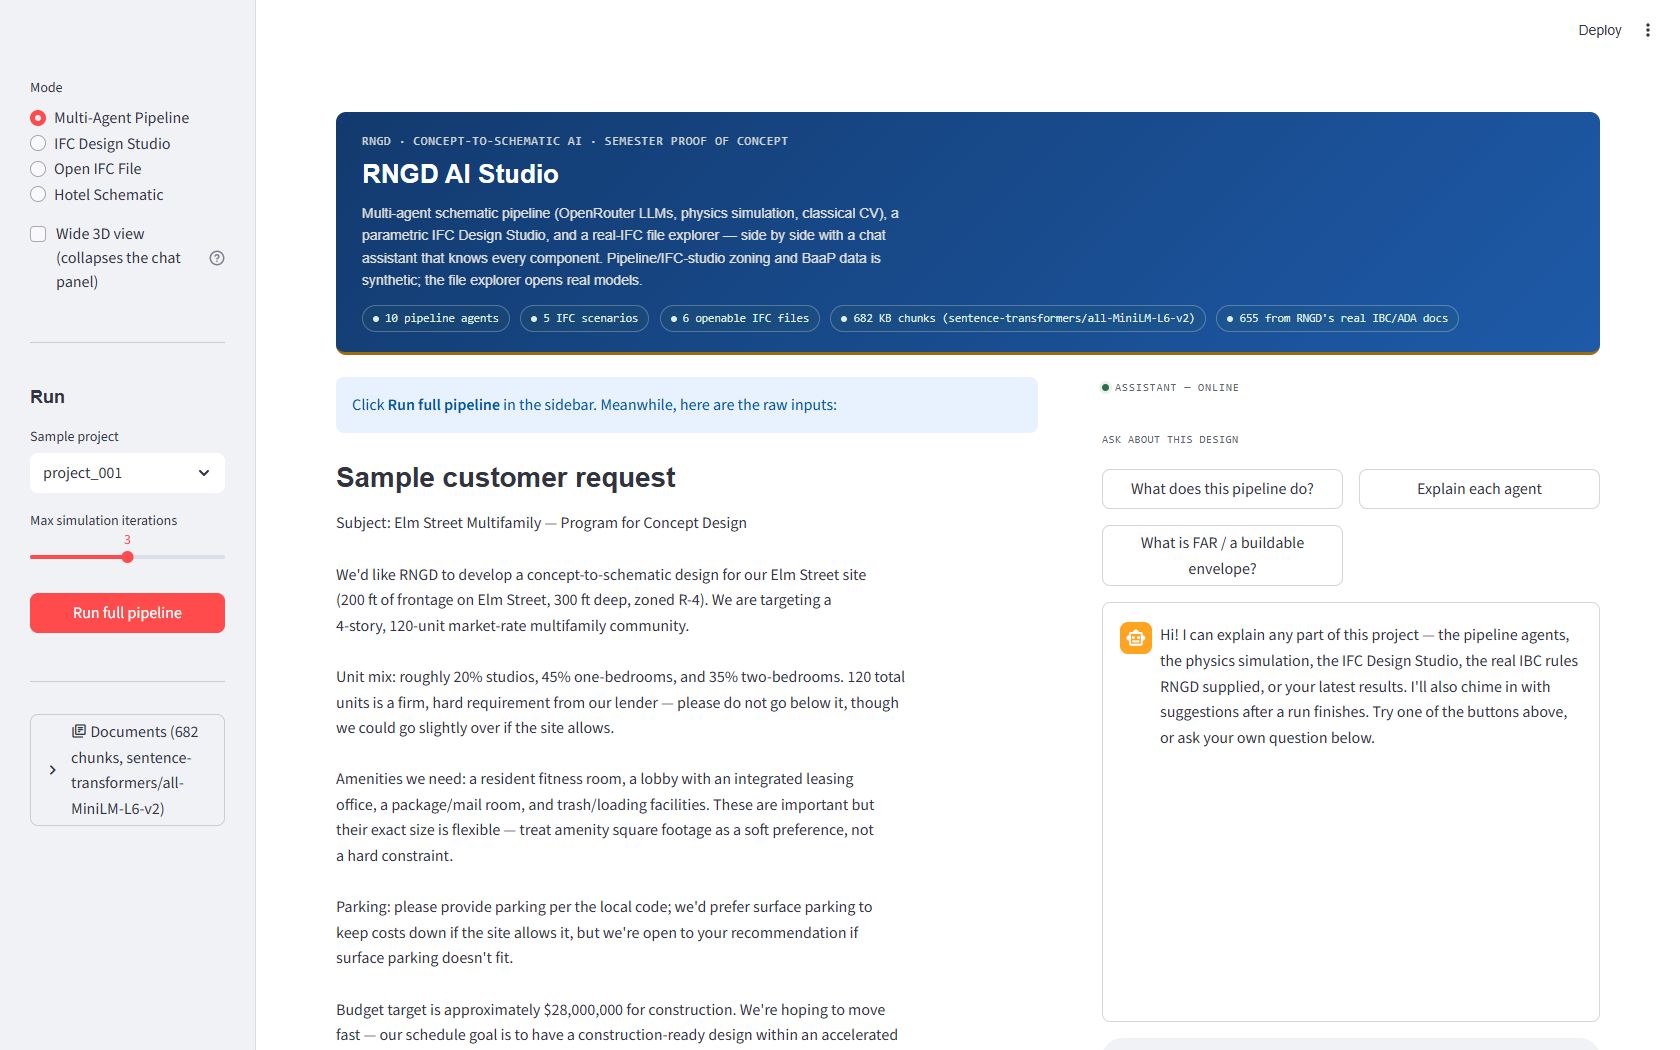
\includegraphics[width=\linewidth,keepaspectratio,height=0.42\textheight]{screens/01_pipeline_inputs.png}\caption{Multi-Agent Pipeline before a run: the sample customer request and site sketch that feed the agents; the assistant panel on the right.}\end{figure}
\begin{figure}[H]\centering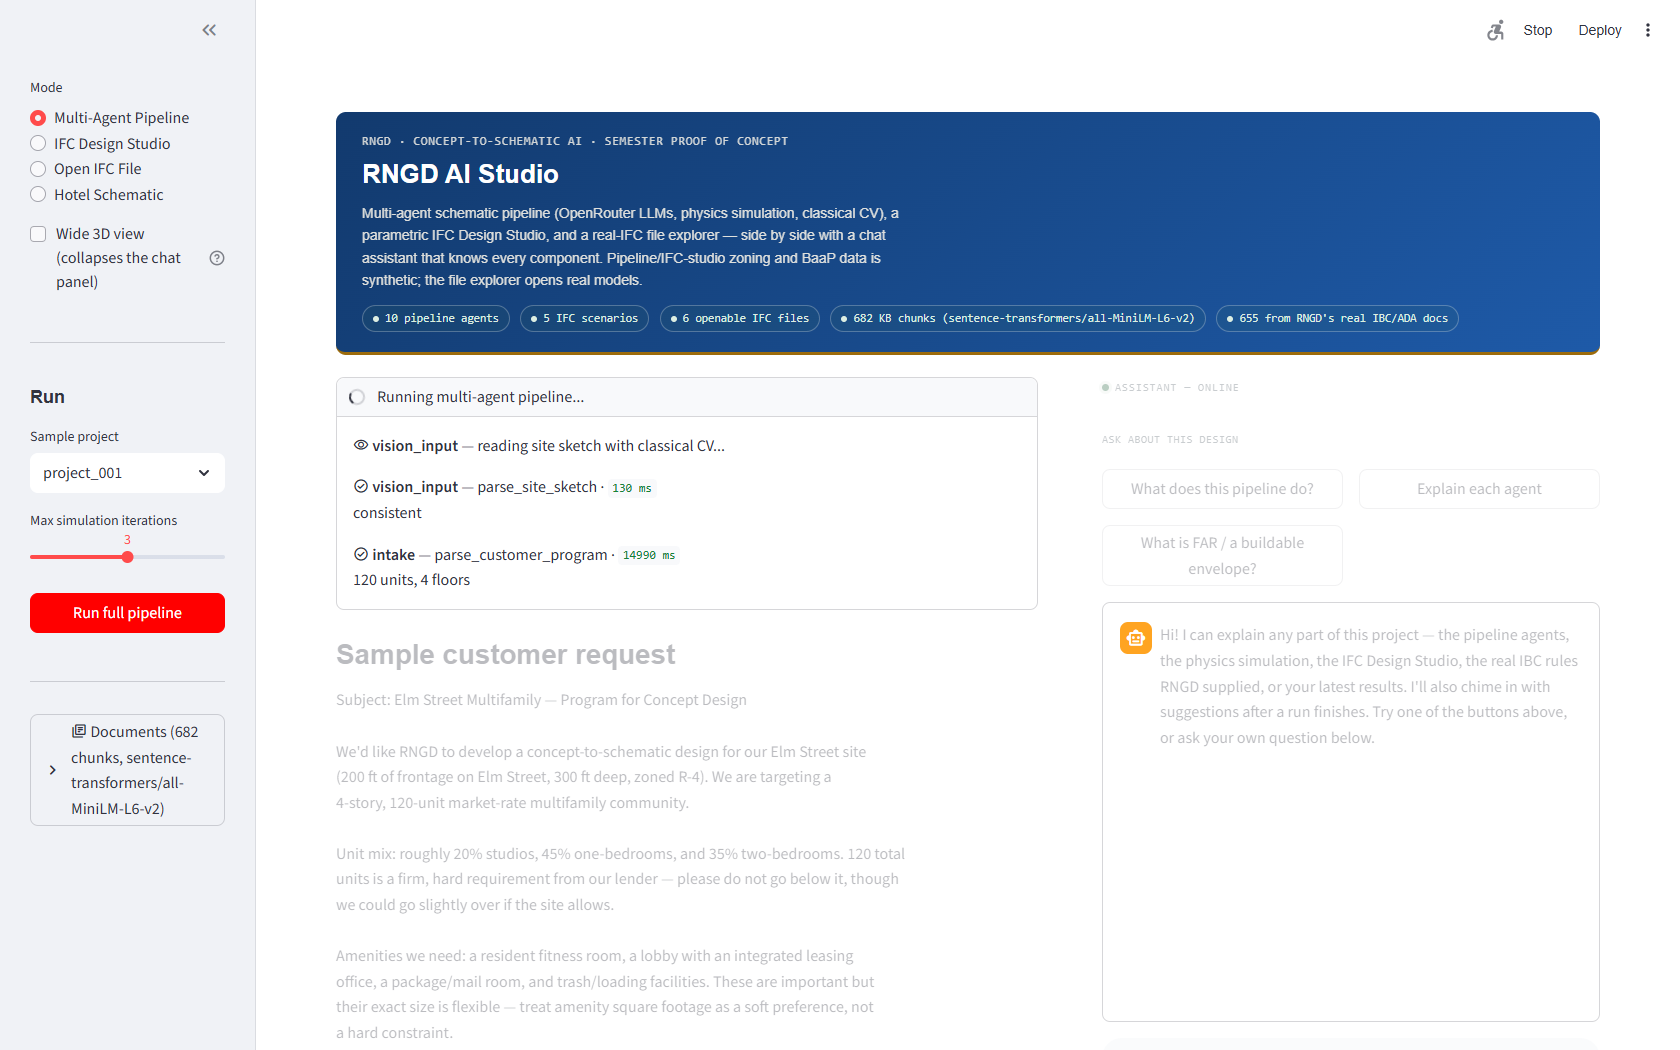
\includegraphics[width=\linewidth,keepaspectratio,height=0.42\textheight]{screens/02_pipeline_running.png}\caption{The pipeline running live: each agent reports its step as it finishes.}\end{figure}
\begin{figure}[H]\centering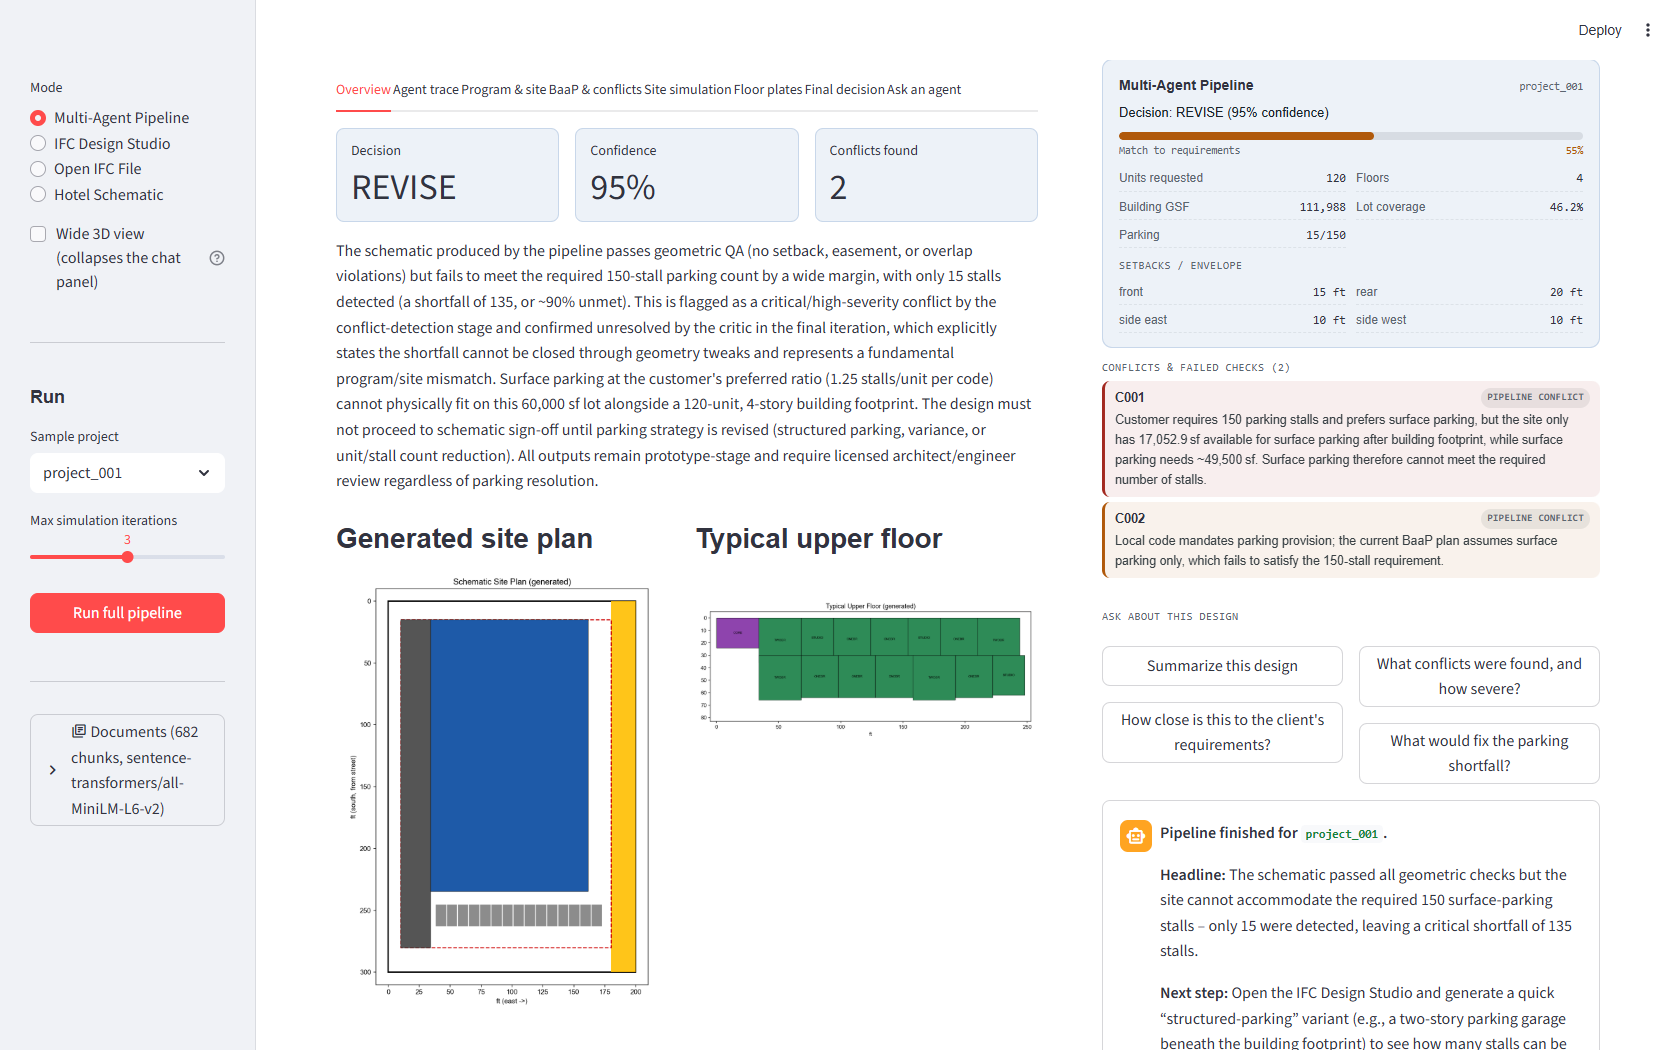
\includegraphics[width=\linewidth,keepaspectratio,height=0.42\textheight]{screens/03_pipeline_overview.png}\caption{Pipeline result overview: the arbiter's decision, confidence and conflict count.}\end{figure}
\begin{figure}[H]\centering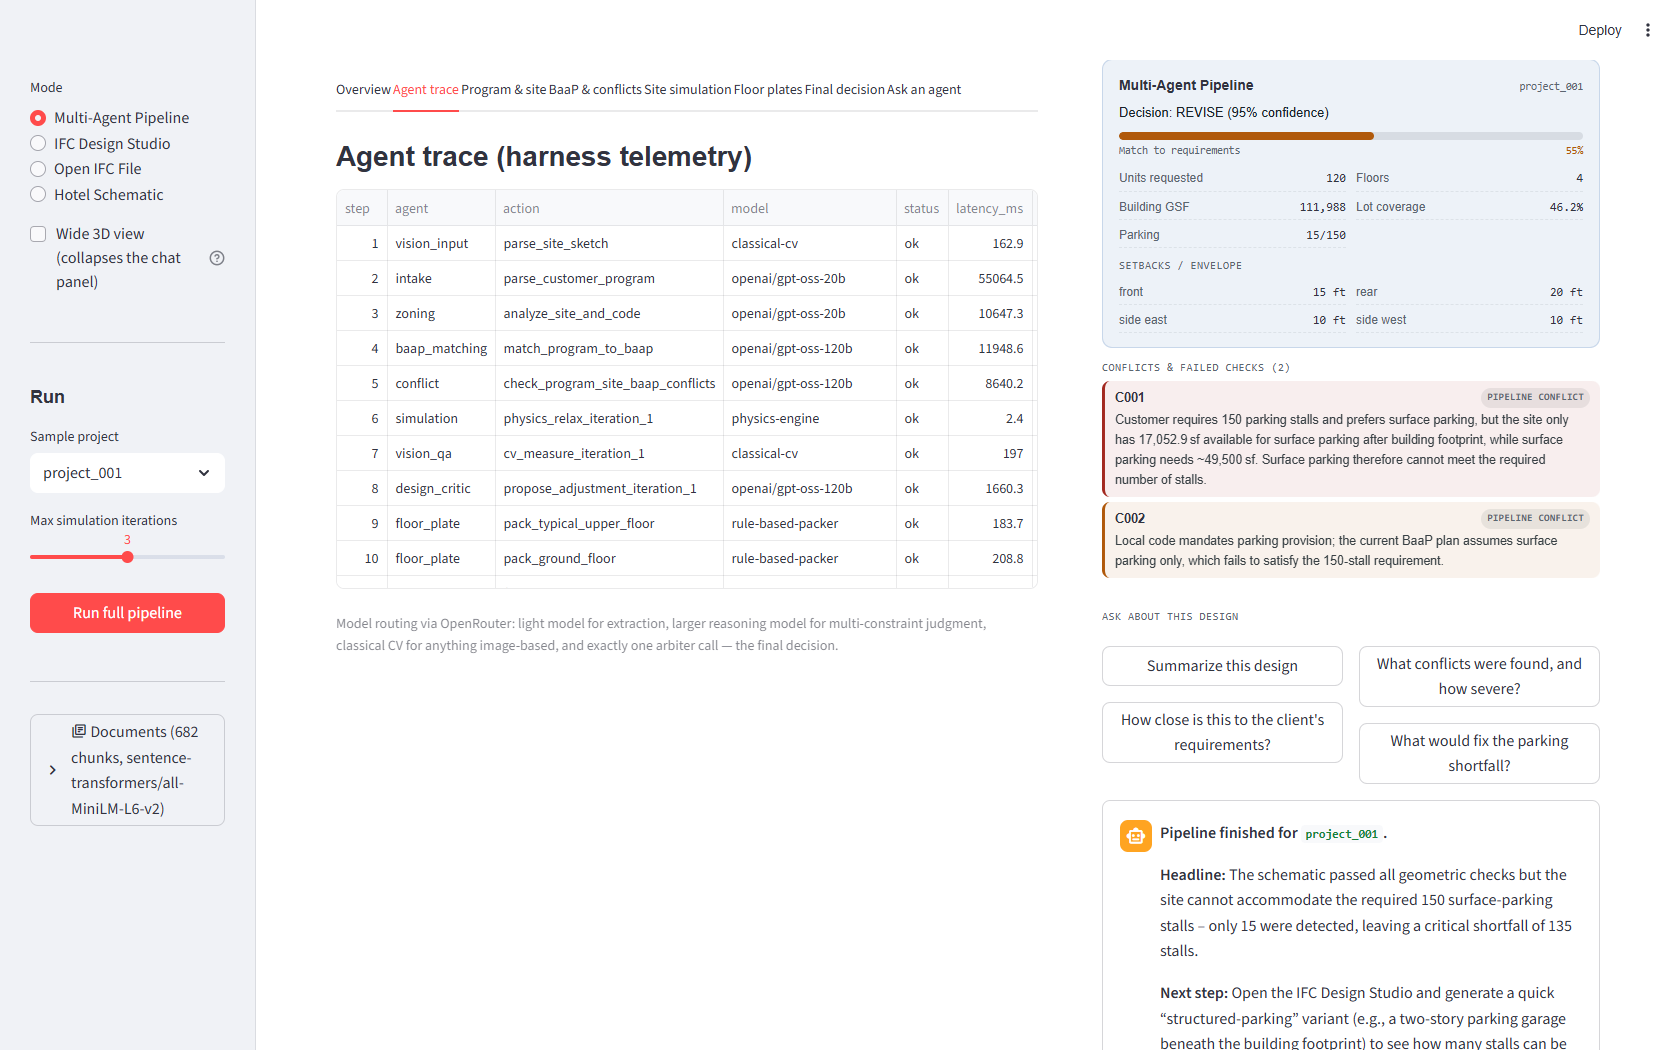
\includegraphics[width=\linewidth,keepaspectratio,height=0.42\textheight]{screens/04_pipeline_agent_trace.png}\caption{Agent trace: every agent step with model, status and latency.}\end{figure}
\begin{figure}[H]\centering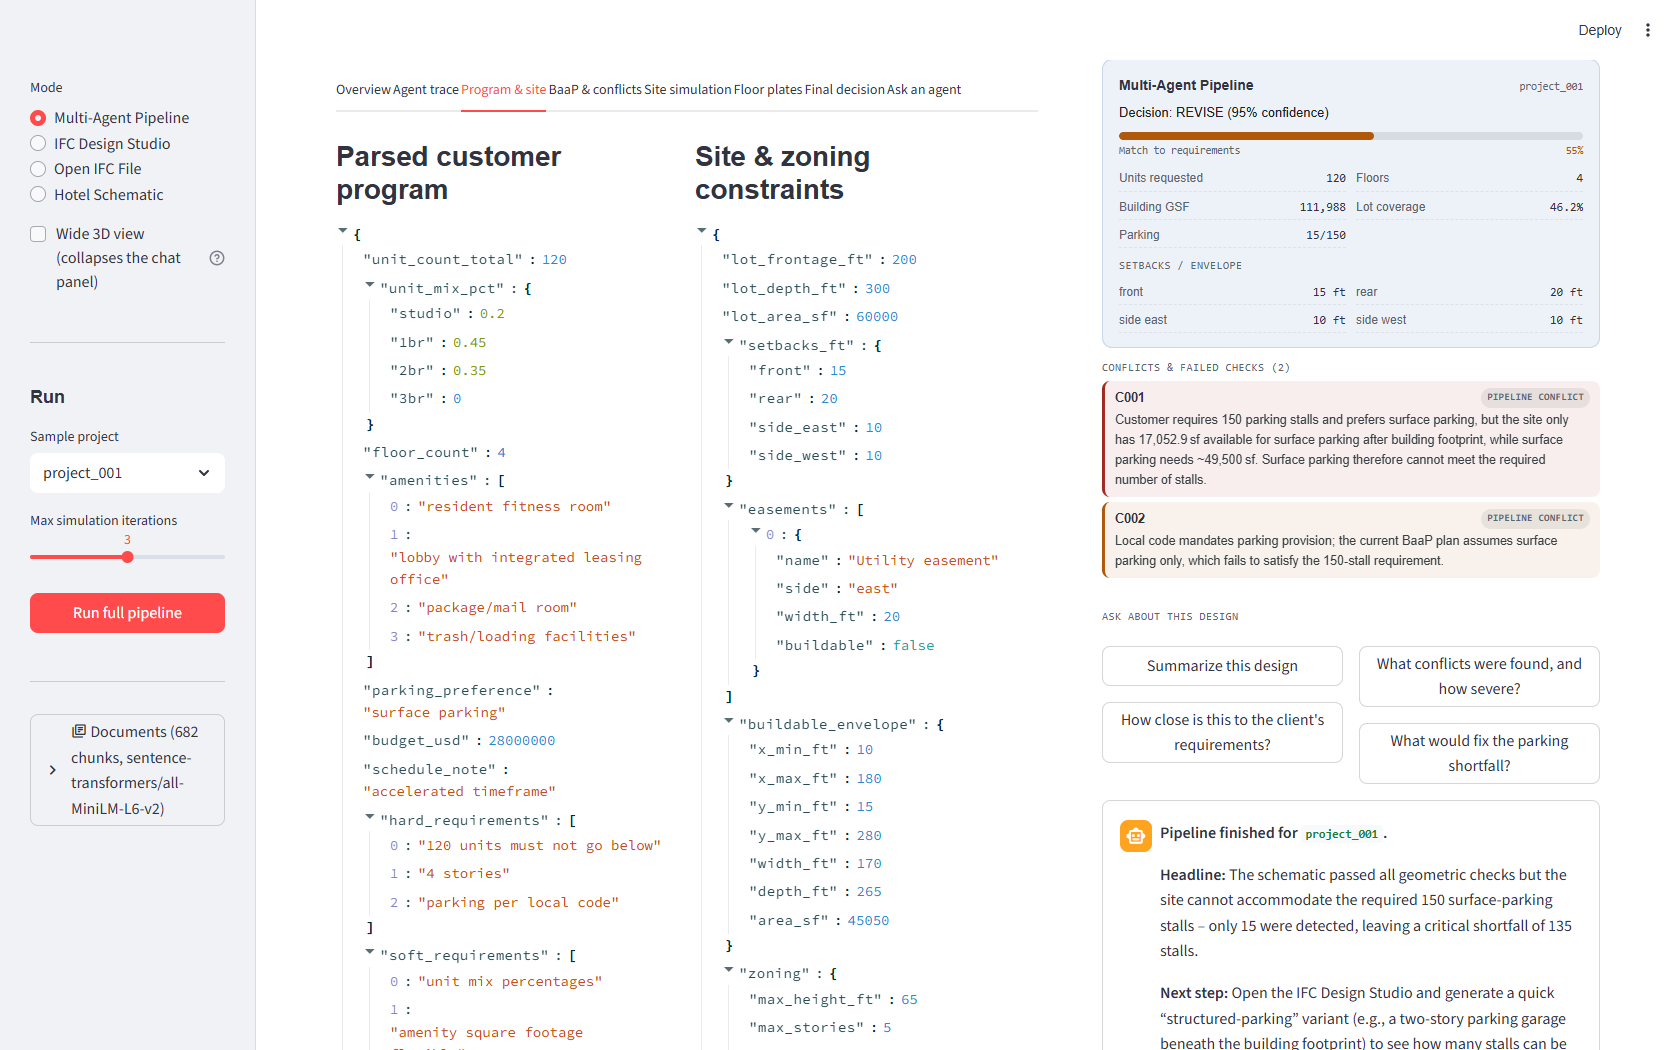
\includegraphics[width=\linewidth,keepaspectratio,height=0.42\textheight]{screens/05_pipeline_program_site.png}\caption{Program parsed from the request and the computed site constraints.}\end{figure}
\begin{figure}[H]\centering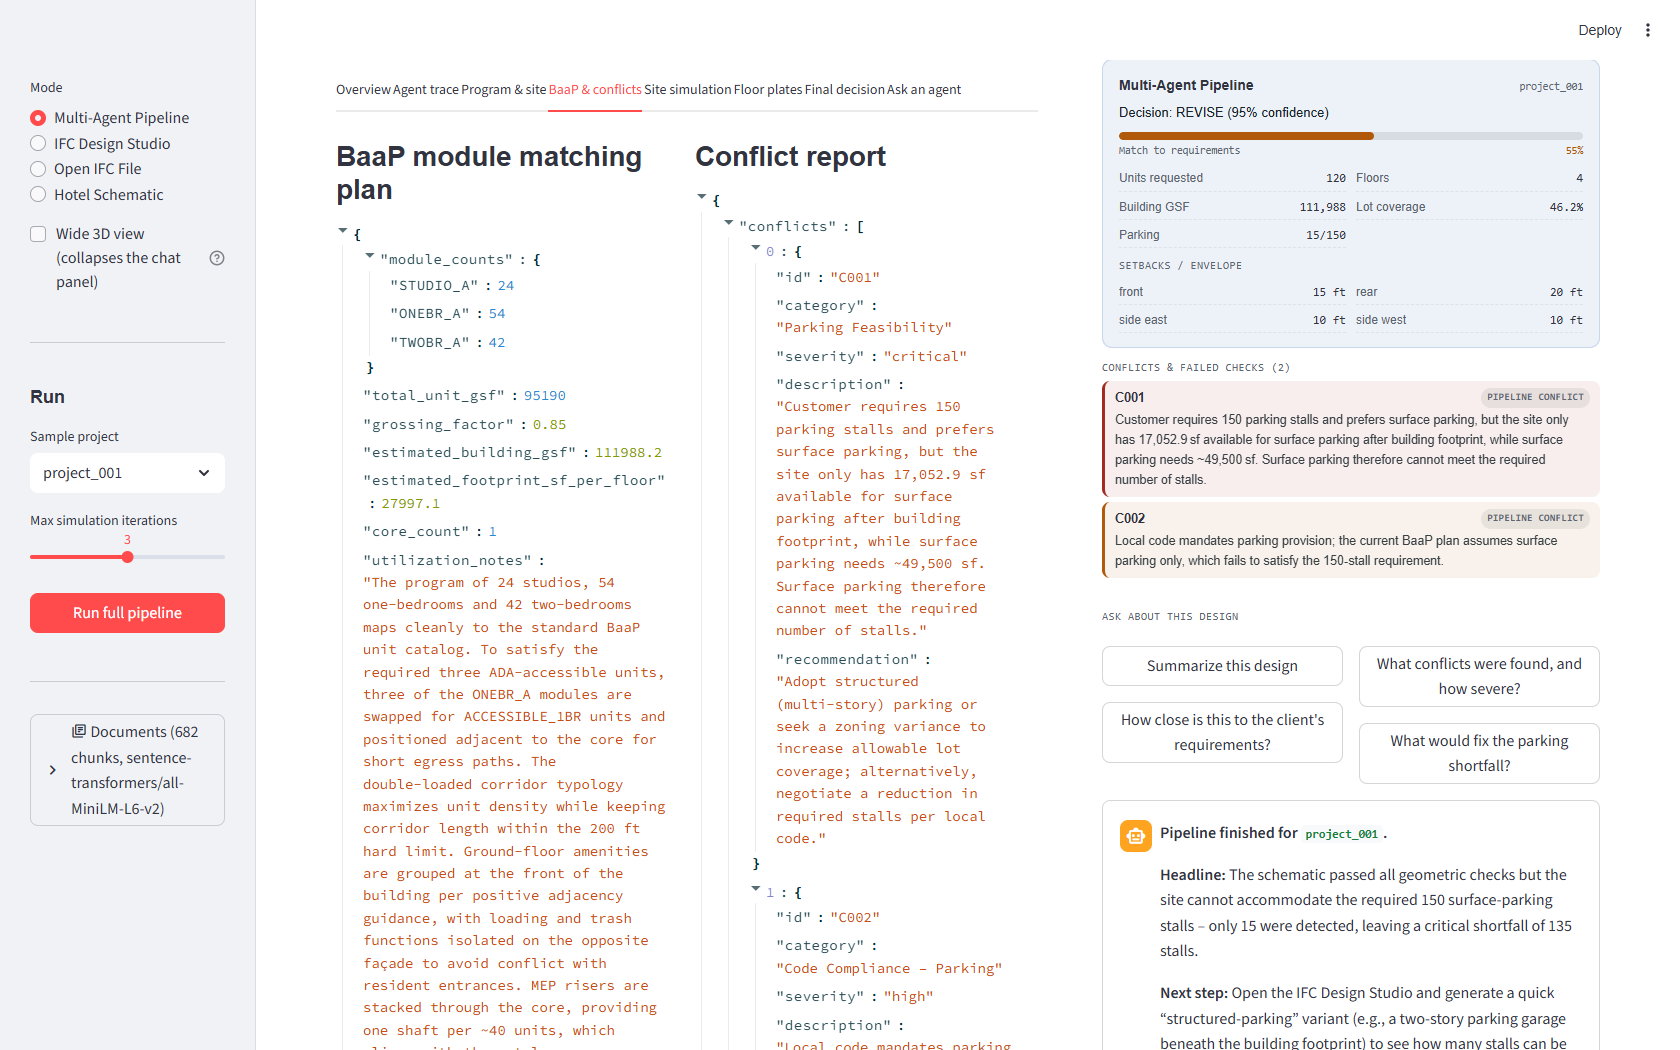
\includegraphics[width=\linewidth,keepaspectratio,height=0.42\textheight]{screens/06_pipeline_baap_conflicts.png}\caption{BaaP module counts and the conflicts the Conflict Agent found.}\end{figure}
\begin{figure}[H]\centering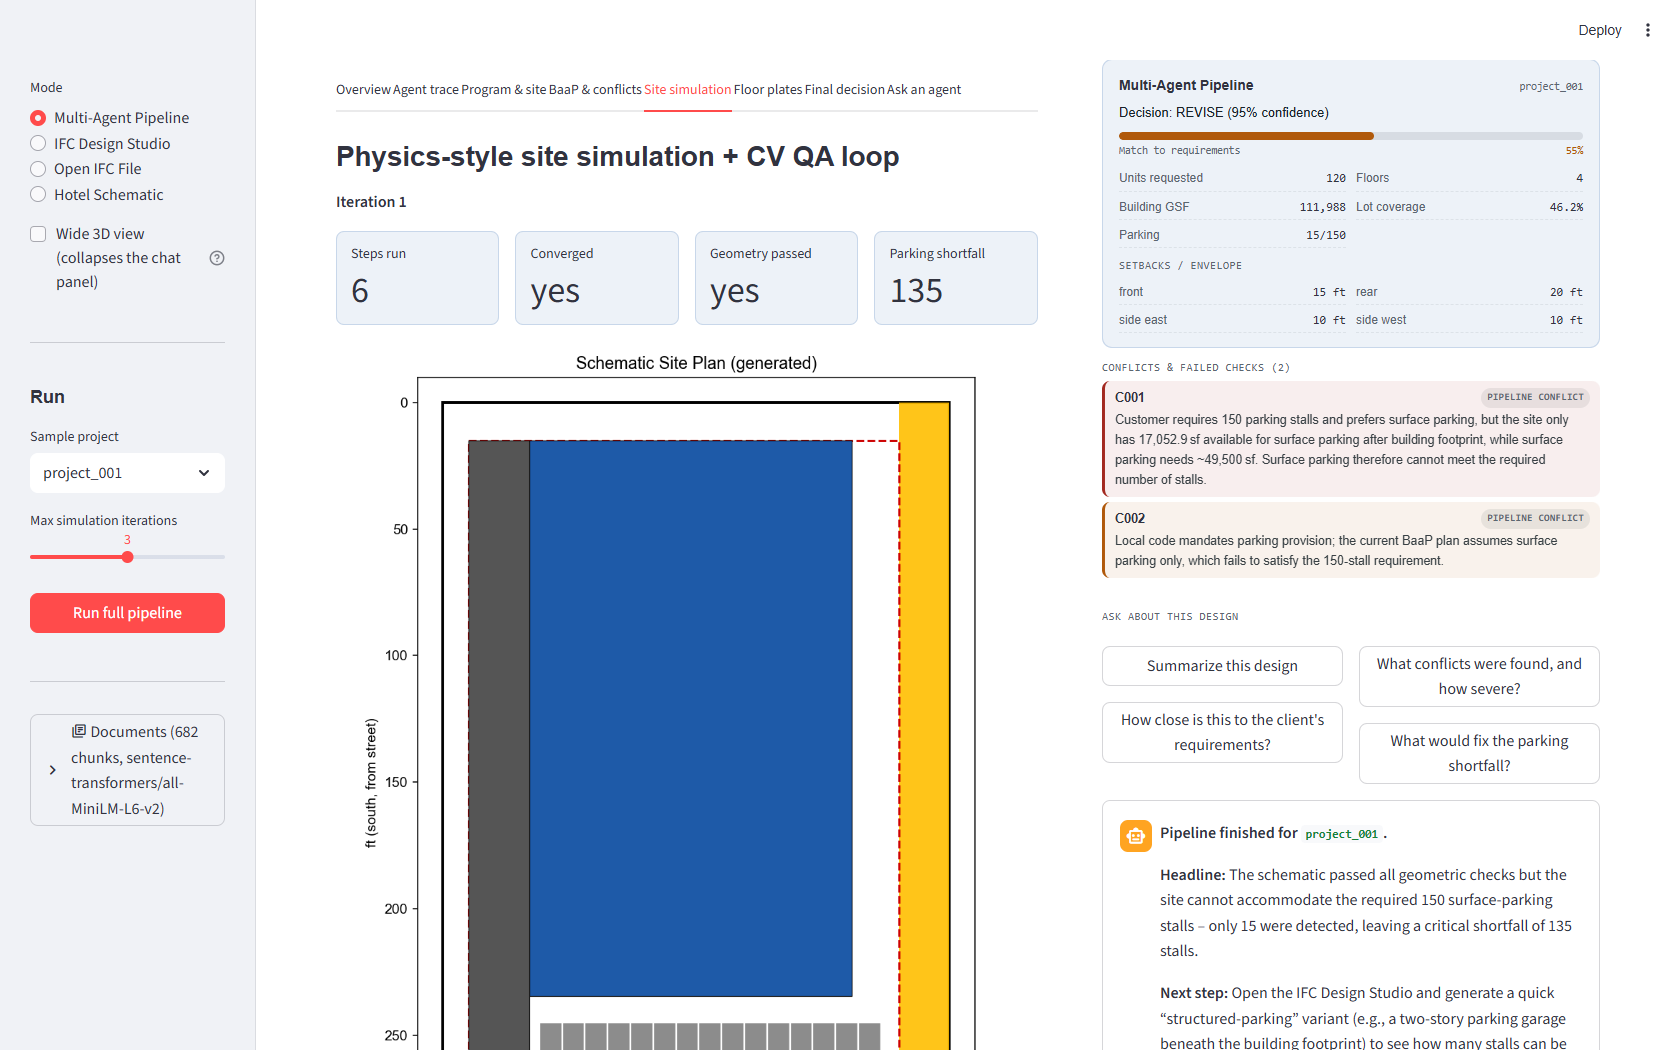
\includegraphics[width=\linewidth,keepaspectratio,height=0.42\textheight]{screens/07_pipeline_site_simulation.png}\caption{Physics-style site simulation and the computer-vision QA of the rendered plan.}\end{figure}
\begin{figure}[H]\centering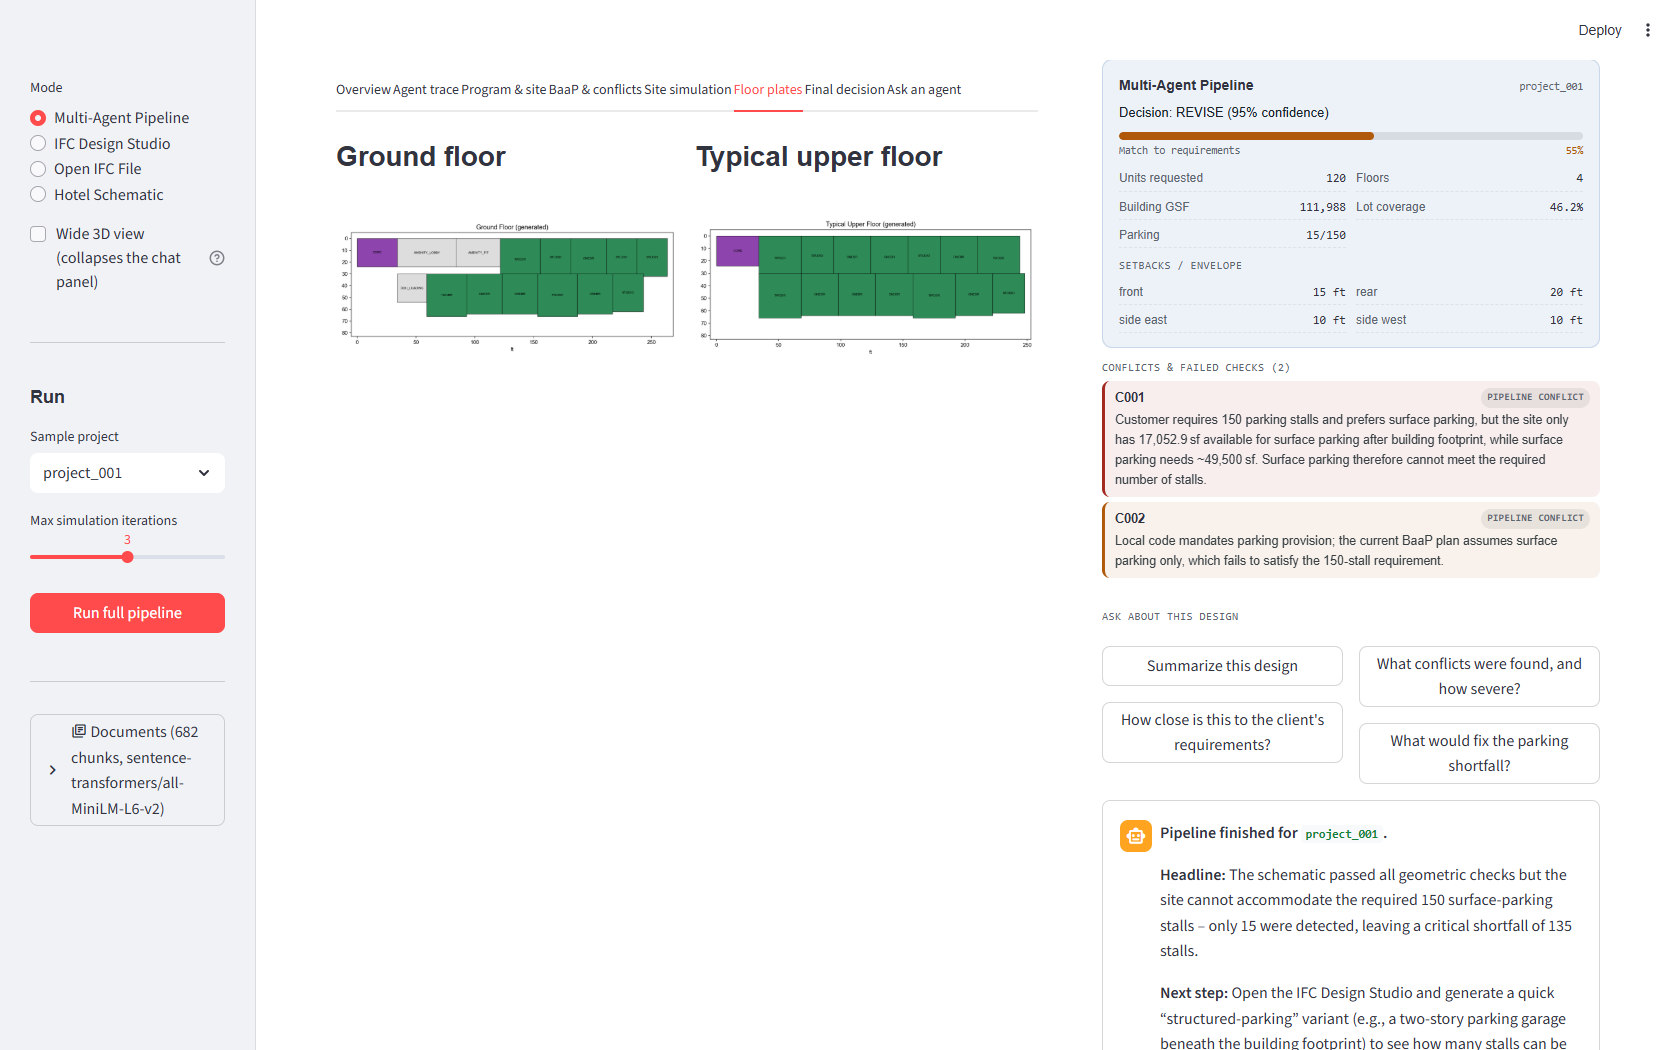
\includegraphics[width=\linewidth,keepaspectratio,height=0.42\textheight]{screens/08_pipeline_floor_plates.png}\caption{Rule-based floor plates (ground and typical floor).}\end{figure}
\begin{figure}[H]\centering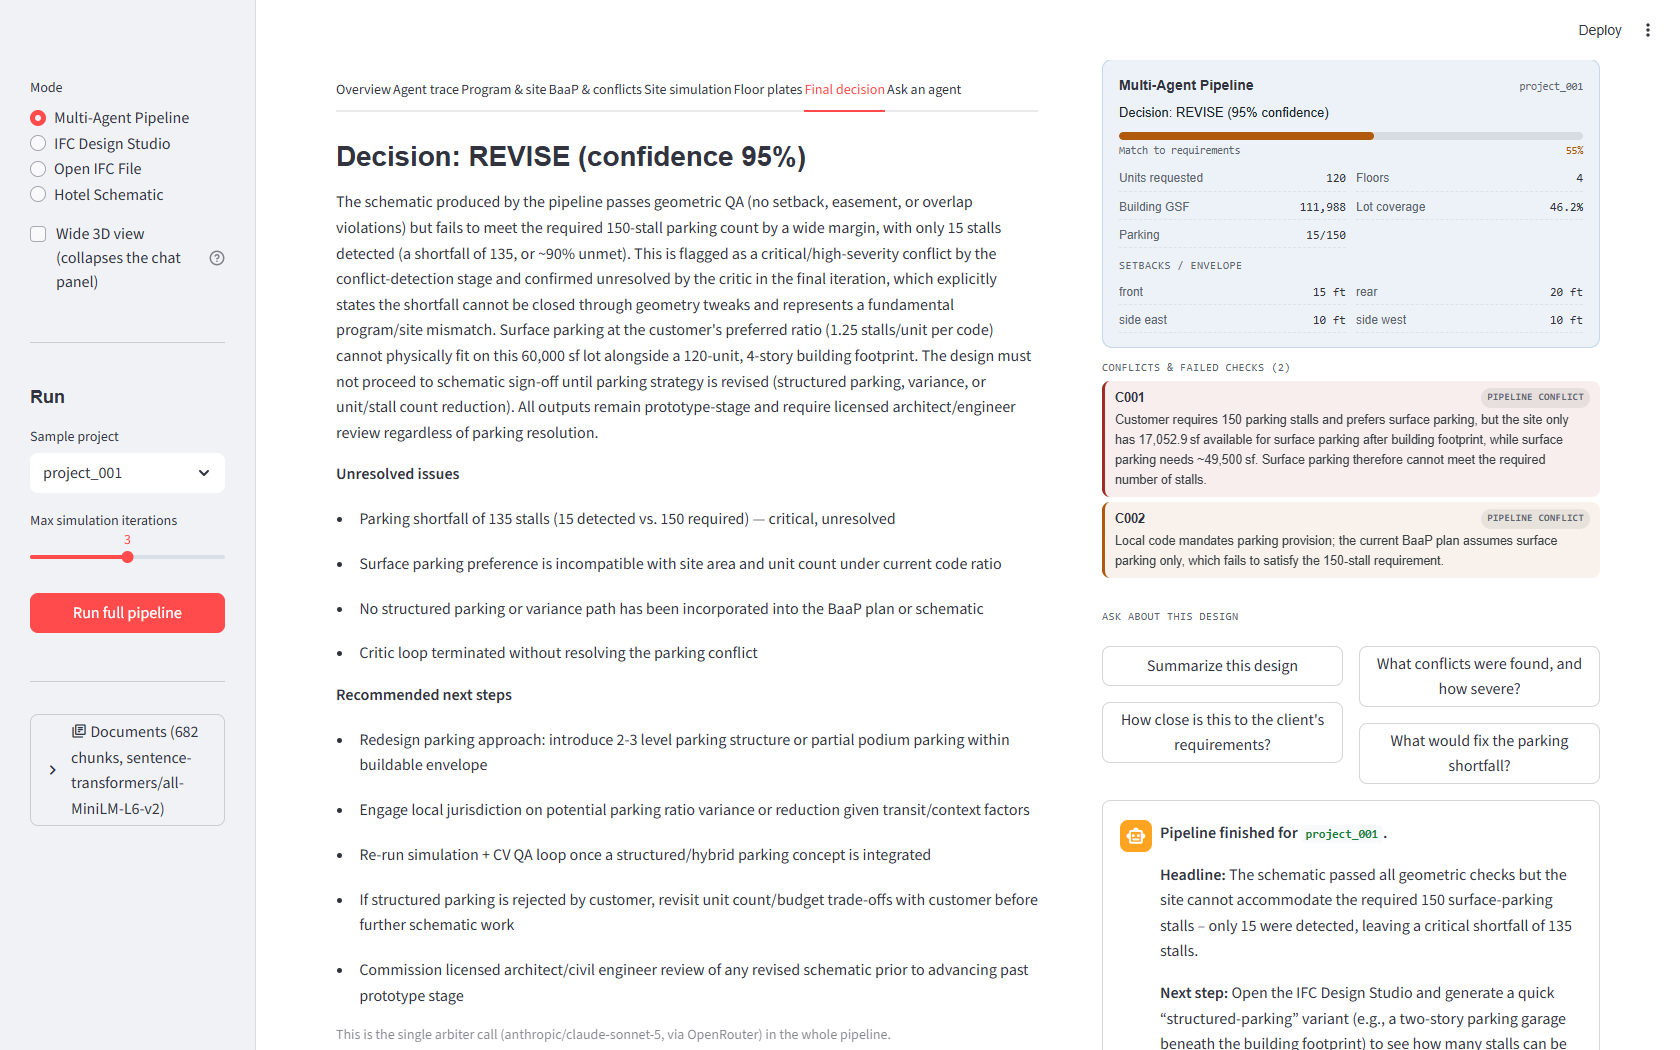
\includegraphics[width=\linewidth,keepaspectratio,height=0.42\textheight]{screens/09_pipeline_final_decision.png}\caption{The arbiter's final decision, unresolved issues and next steps.}\end{figure}


\section{IFC Design Studio (parametric IFC4 generator)}
\subsection{What it does}
A deterministic generator: requirements + a zoning preset + the BaaP catalog produce a building layout, written as a
real IFC4 file with IfcOpenShell and shown in an interactive 3D viewer. Every design is scored against ten
sample-zoning checks and cross-checked against a subset of RNGD's real 2021 IBC rules. Zoning presets are synthetic.

\subsection{All five scenarios}
{\small \begin{longtable}{p{4.4cm}p{1.2cm}p{1.0cm}p{0.8cm}p{1.3cm}p{1.4cm}p{1.8cm}p{2.6cm}}
\toprule
\textbf{Scenario} & \textbf{Units} & \textbf{Stories} & \textbf{FAR} & \textbf{Coverage} & \textbf{Parking} & \textbf{Sample zoning} & \textbf{Real IBC} \\ \midrule \endhead
Baseline: 4 floors, surface parking & 120/120 & 4 & 3.16 & 79.1\% & 23/150 & \textcolor{fail}{4 fail} & \textcolor{fail}{IBC-R1-027} \\
Right-sized: 60 units, podium (compliant) & 60/60 & 5 & 2.31 & 46.3\% & 75/75 & \textcolor{pass}{\textbf{PASS}} & \textcolor{fail}{IBC-R1-027} \\
Podium parking, 5 floors & 120/120 & 6 & 3.74 & 62.4\% & 120/150 & \textcolor{fail}{7 fail} & \textcolor{fail}{IBC-R1-007, IBC-R1-008, IBC-R1-027} \\
Dense R-6, 7 floors + podium & 120/120 & 8 & 4.01 & 50.2\% & 90/90 & \textcolor{fail}{3 fail} & \textcolor{fail}{IBC-R1-005, IBC-R1-006, IBC-R1-007, IBC-R1-008, IBC-R1-027} \\
Suburban R-2, 60 units, 3 floors & 60/60 & 3 & 1.62 & 54.1\% & 10/120 & \textcolor{fail}{3 fail} & \textcolor{fail}{IBC-R1-027} \\
\bottomrule
\end{longtable}}

\subsection{Baseline vs right-sized}
Side by side: the Baseline (120 units, surface parking) and the Right-sized scenario (60 units, podium parking)
that the app offers as the fix.
{\small \begin{longtable}{p{4.4cm}p{2.4cm}p{2.2cm}p{1.2cm}p{2.2cm}p{1.2cm}}
\toprule
\textbf{Check} & \textbf{Required} & \textbf{Baseline} & \textbf{} & \textbf{Right-sized} & \textbf{} \\ \midrule \endhead
Units placed & 120 & 120 & \textcolor{pass}{\textbf{PASS}} & 60 & \textcolor{pass}{\textbf{PASS}} \\
Stories & $\le$ 5 & 4 & \textcolor{pass}{\textbf{PASS}} & 5 & \textcolor{pass}{\textbf{PASS}} \\
Height (ft) & $\le$ 65 & 45.5 & \textcolor{pass}{\textbf{PASS}} & 56.0 & \textcolor{pass}{\textbf{PASS}} \\
FAR & $\le$ 2.5 & 3.16 & \textcolor{fail}{\textbf{FAIL}} & 2.31 & \textcolor{pass}{\textbf{PASS}} \\
Lot coverage \% & $\le$ 60 & 79.1 & \textcolor{fail}{\textbf{FAIL}} & 46.3 & \textcolor{pass}{\textbf{PASS}} \\
Parking stalls & 150 & 23 & \textcolor{fail}{\textbf{FAIL}} & 75 & \textcolor{pass}{\textbf{PASS}} \\
Building inside setbacks/easement & yes & no & \textcolor{fail}{\textbf{FAIL}} & yes & \textcolor{pass}{\textbf{PASS}} \\
Fire lane / driveway (24 ft) & yes & yes & \textcolor{pass}{\textbf{PASS}} & yes & \textcolor{pass}{\textbf{PASS}} \\
Accessible units (2\%) & 3 & 3 & \textcolor{pass}{\textbf{PASS}} & 2 & \textcolor{pass}{\textbf{PASS}} \\
Exit travel to core (ft) & $\le$ 200 & 180 & \textcolor{pass}{\textbf{PASS}} & 154 & \textcolor{pass}{\textbf{PASS}} \\
\bottomrule
\end{longtable}}

\subsection{Baseline against RNGD's real IBC rules}
{\small \begin{longtable}{p{1.8cm}p{6.2cm}p{2.4cm}p{2.4cm}p{1.4cm}}
\toprule
\textbf{Rule} & \textbf{Rule name} & \textbf{Required} & \textbf{Measured} & \textbf{Status} \\ \midrule \endhead
IBC-R1-005 & R occupancy sprinklered Type IIA allowable height & $\le$ 85 ft & 45.5 & \textcolor{pass}{\textbf{PASS}} \\
IBC-R1-006 & R occupancy sprinklered Type IIB allowable height & $\le$ 75 ft & 45.5 & \textcolor{pass}{\textbf{PASS}} \\
IBC-R1-007 & R-1 sprinklered Type IIA allowable stories & $\le$ 5 stories above grade plane & 4 & \textcolor{pass}{\textbf{PASS}} \\
IBC-R1-008 & R-1 sprinklered Type IIB allowable stories & $\le$ 5 stories above grade plane & 4 & \textcolor{pass}{\textbf{PASS}} \\
IBC-R1-023 & R exit access travel distance, sprinklered & $\le$ 250 ft & 180 & \textcolor{pass}{\textbf{PASS}} \\
IBC-R1-027 & Dead-end corridor maximum for sprinklered R-1 & $\le$ 50 ft & 180 & \textcolor{fail}{\textbf{FAIL}} \\
IBC-R1-015 & Minimum exits per story: 1-500 occupants & 2 exits (occupant load 1-500) & 6 exits (3 core(s) x 2 stairs), \textasciitilde{}140 occupants/floor & \textcolor{pass}{\textbf{PASS}} \\
\bottomrule
\end{longtable}}

\subsection{Screenshots}
\begin{figure}[H]\centering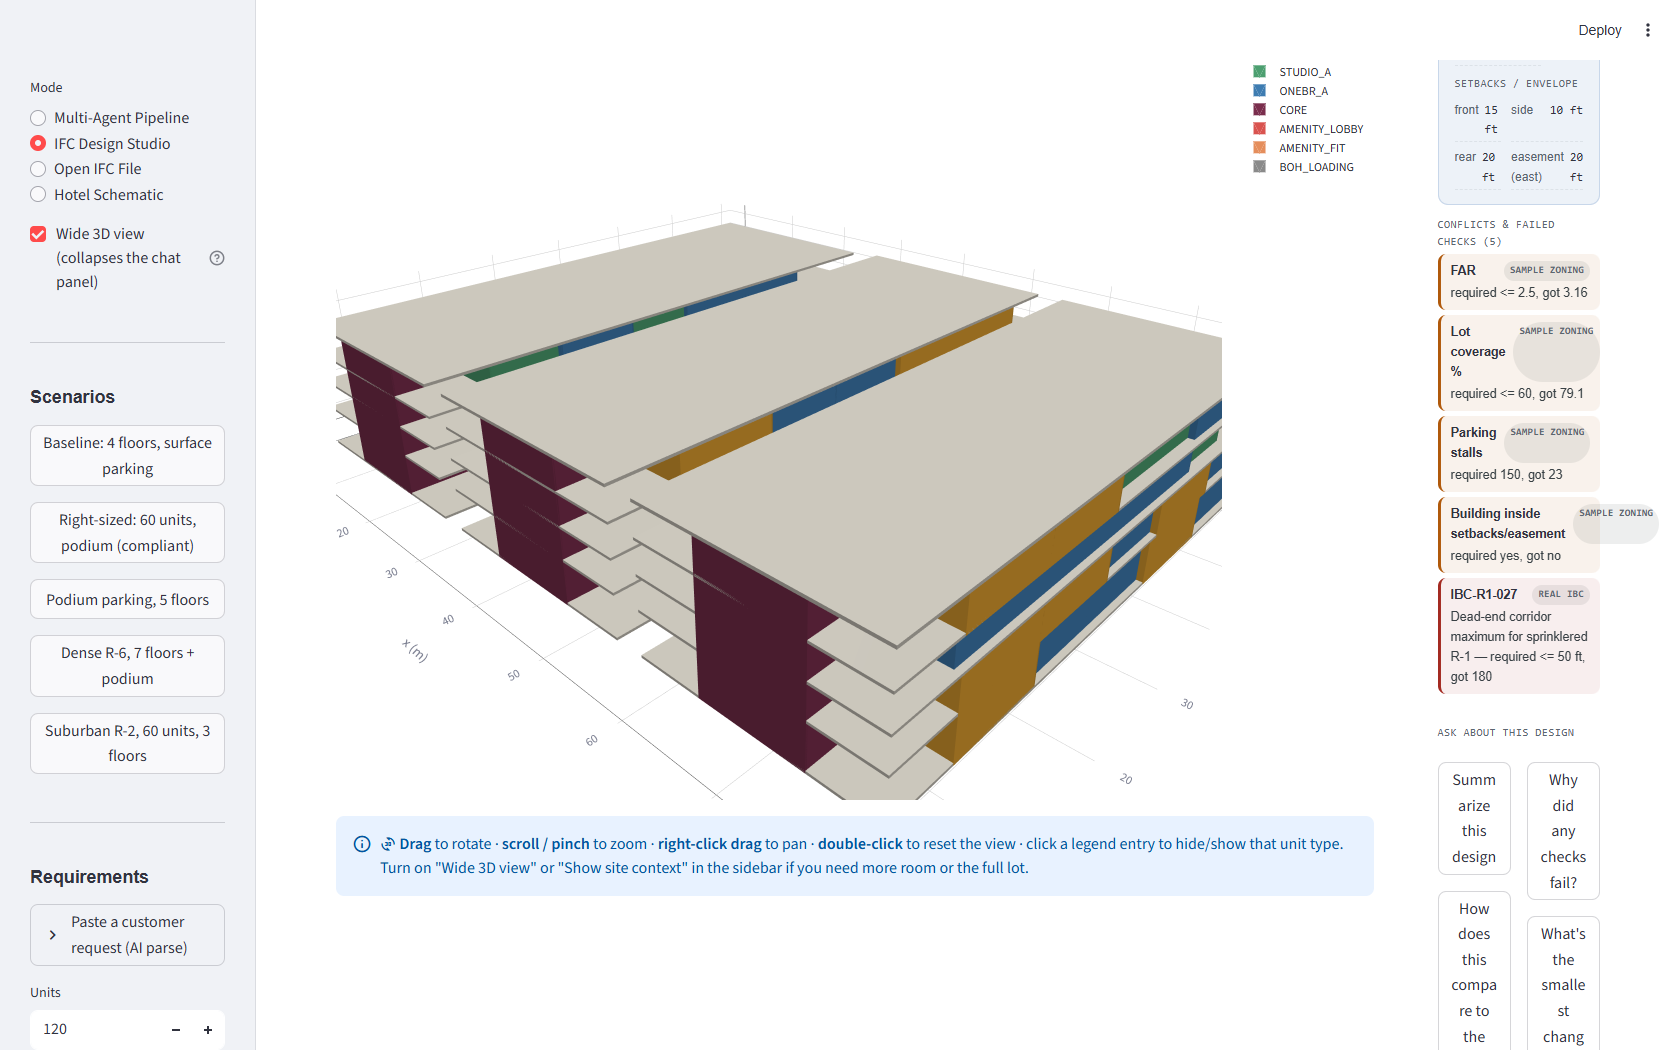
\includegraphics[width=\linewidth,keepaspectratio,height=0.42\textheight]{screens/10_ifc_baseline_3d_model.png}\caption{IFC Design Studio, Baseline scenario (120 units, 4 floors, surface parking): the generated IFC4 model in the 3D viewer.}\end{figure}
\begin{figure}[H]\centering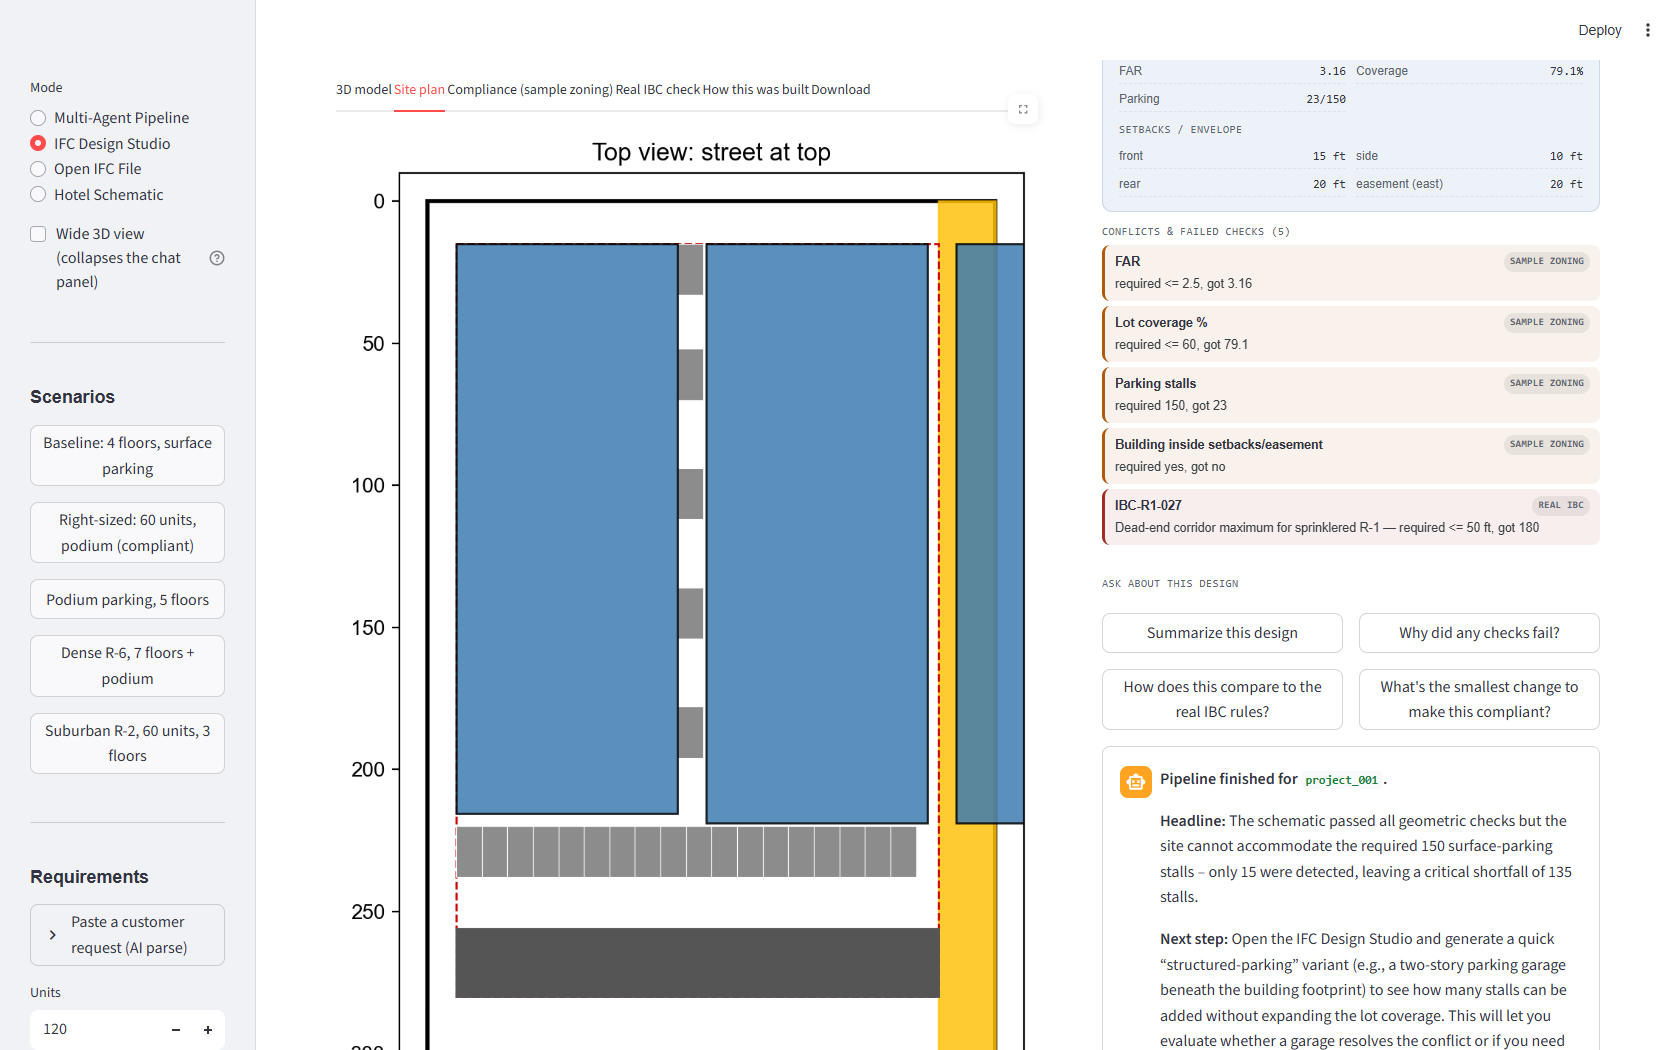
\includegraphics[width=\linewidth,keepaspectratio,height=0.42\textheight]{screens/11_ifc_baseline_site_plan.png}\caption{Baseline site plan: building, parking, easement and fire lane on the synthetic lot.}\end{figure}
\begin{figure}[H]\centering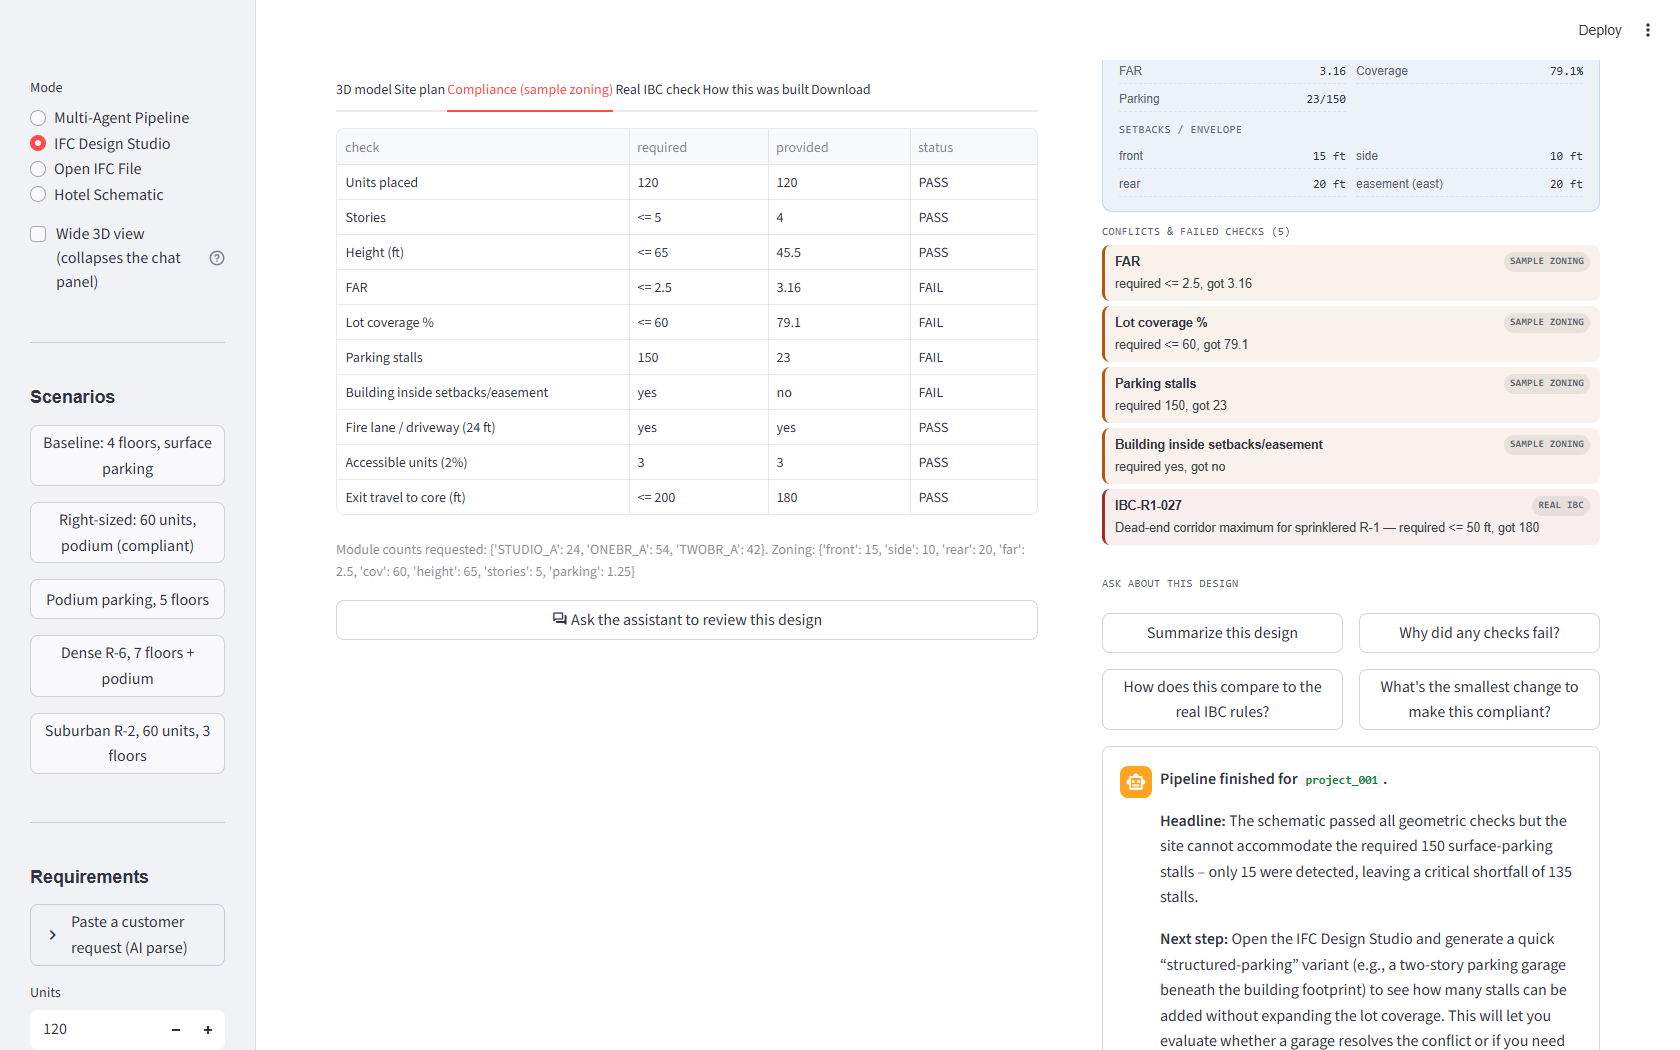
\includegraphics[width=\linewidth,keepaspectratio,height=0.42\textheight]{screens/12_ifc_baseline_compliance.png}\caption{Baseline compliance against the ten sample-zoning checks.}\end{figure}
\begin{figure}[H]\centering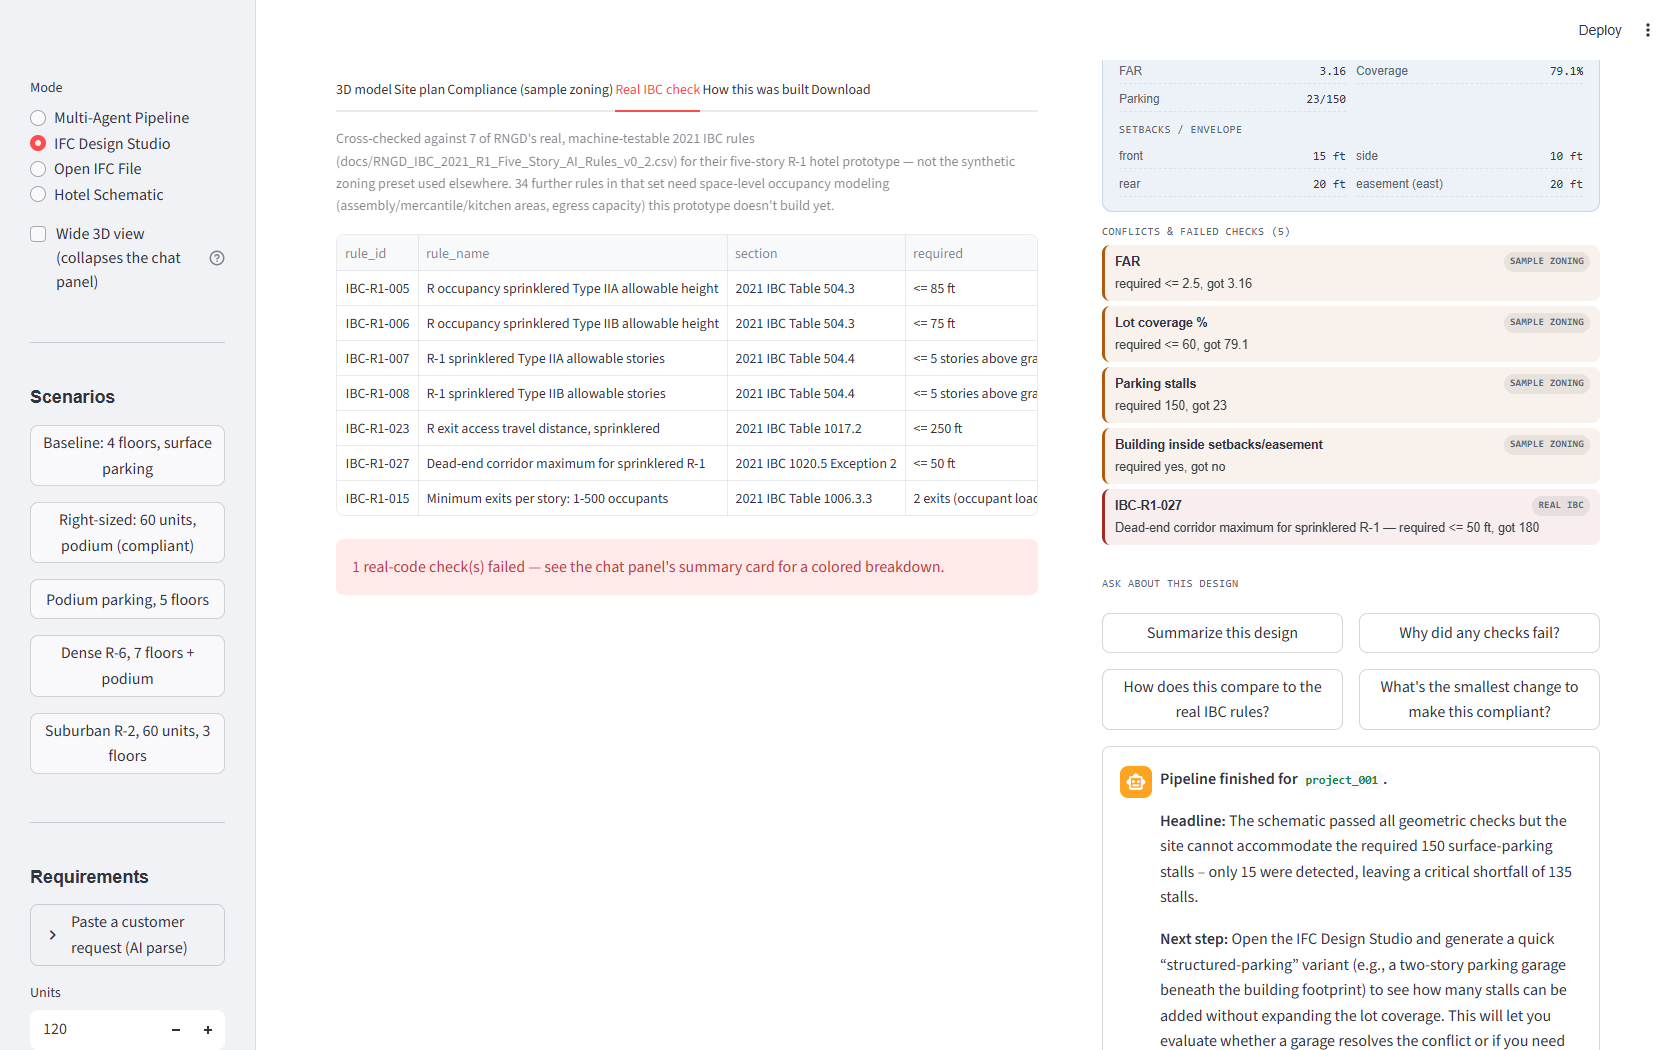
\includegraphics[width=\linewidth,keepaspectratio,height=0.42\textheight]{screens/13_ifc_baseline_real_ibc_check.png}\caption{Baseline cross-checked against RNGD's real 2021 IBC rules.}\end{figure}
\begin{figure}[H]\centering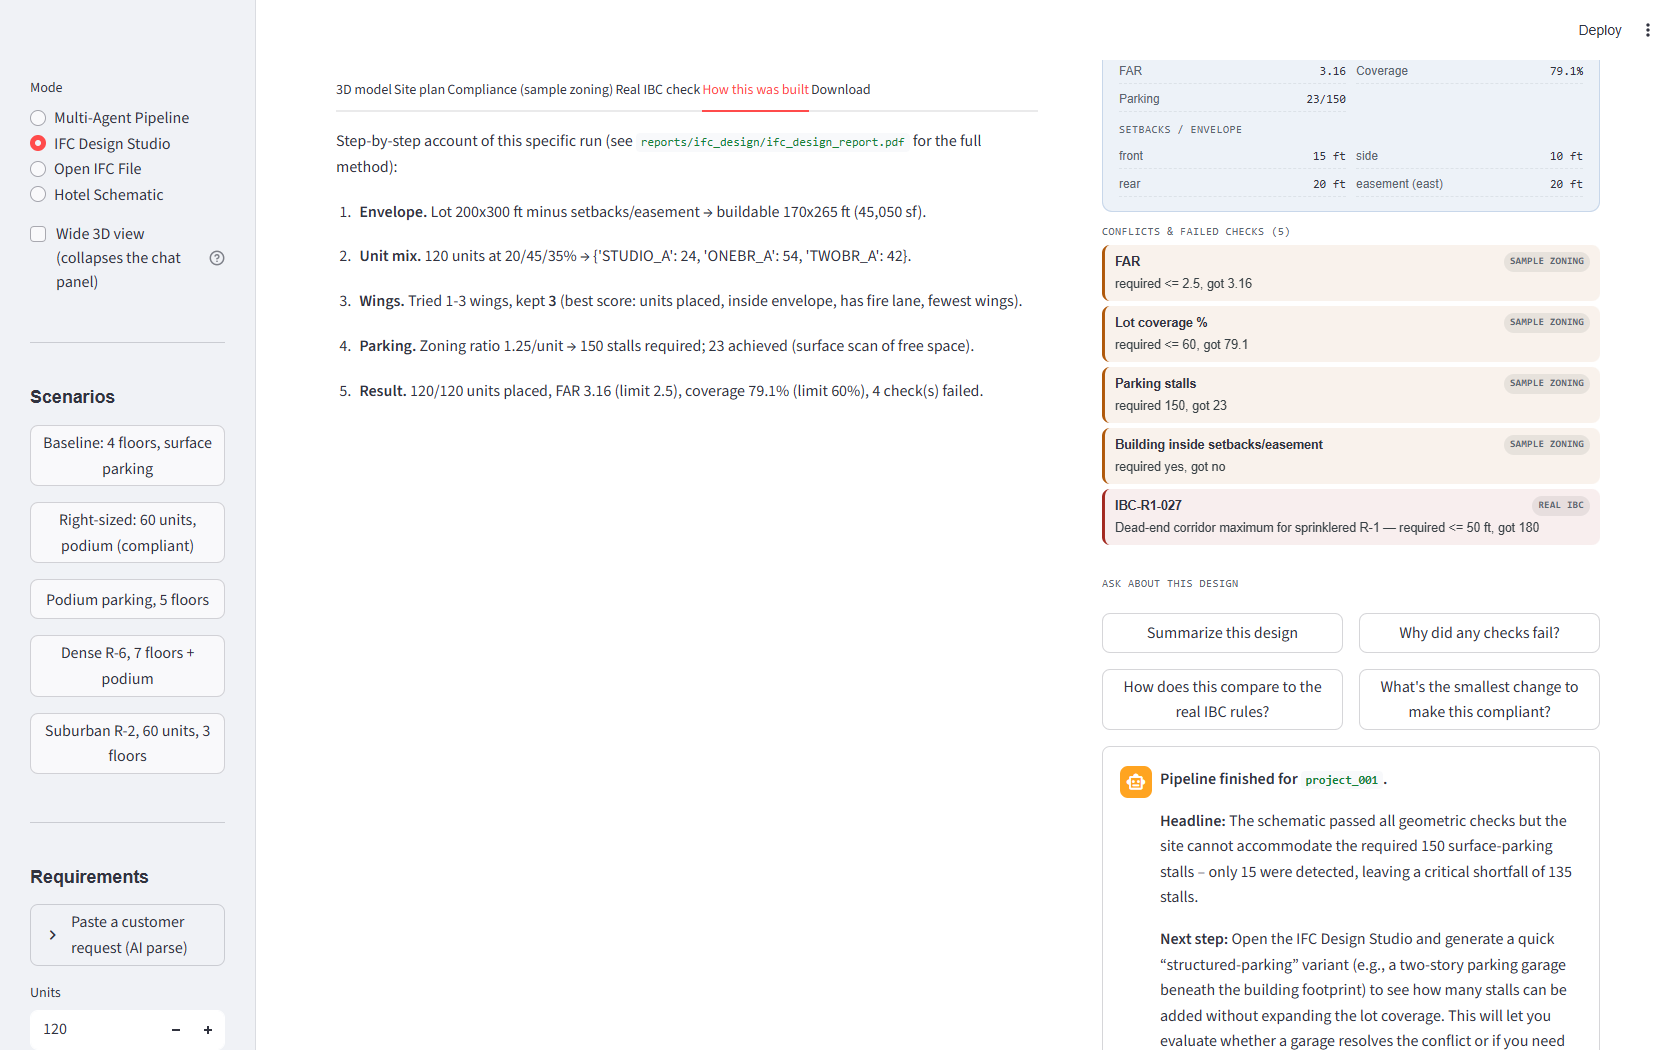
\includegraphics[width=\linewidth,keepaspectratio,height=0.42\textheight]{screens/14_ifc_baseline_how_this_was_built.png}\caption{Step-by-step explanation of how the layout was generated.}\end{figure}
\begin{figure}[H]\centering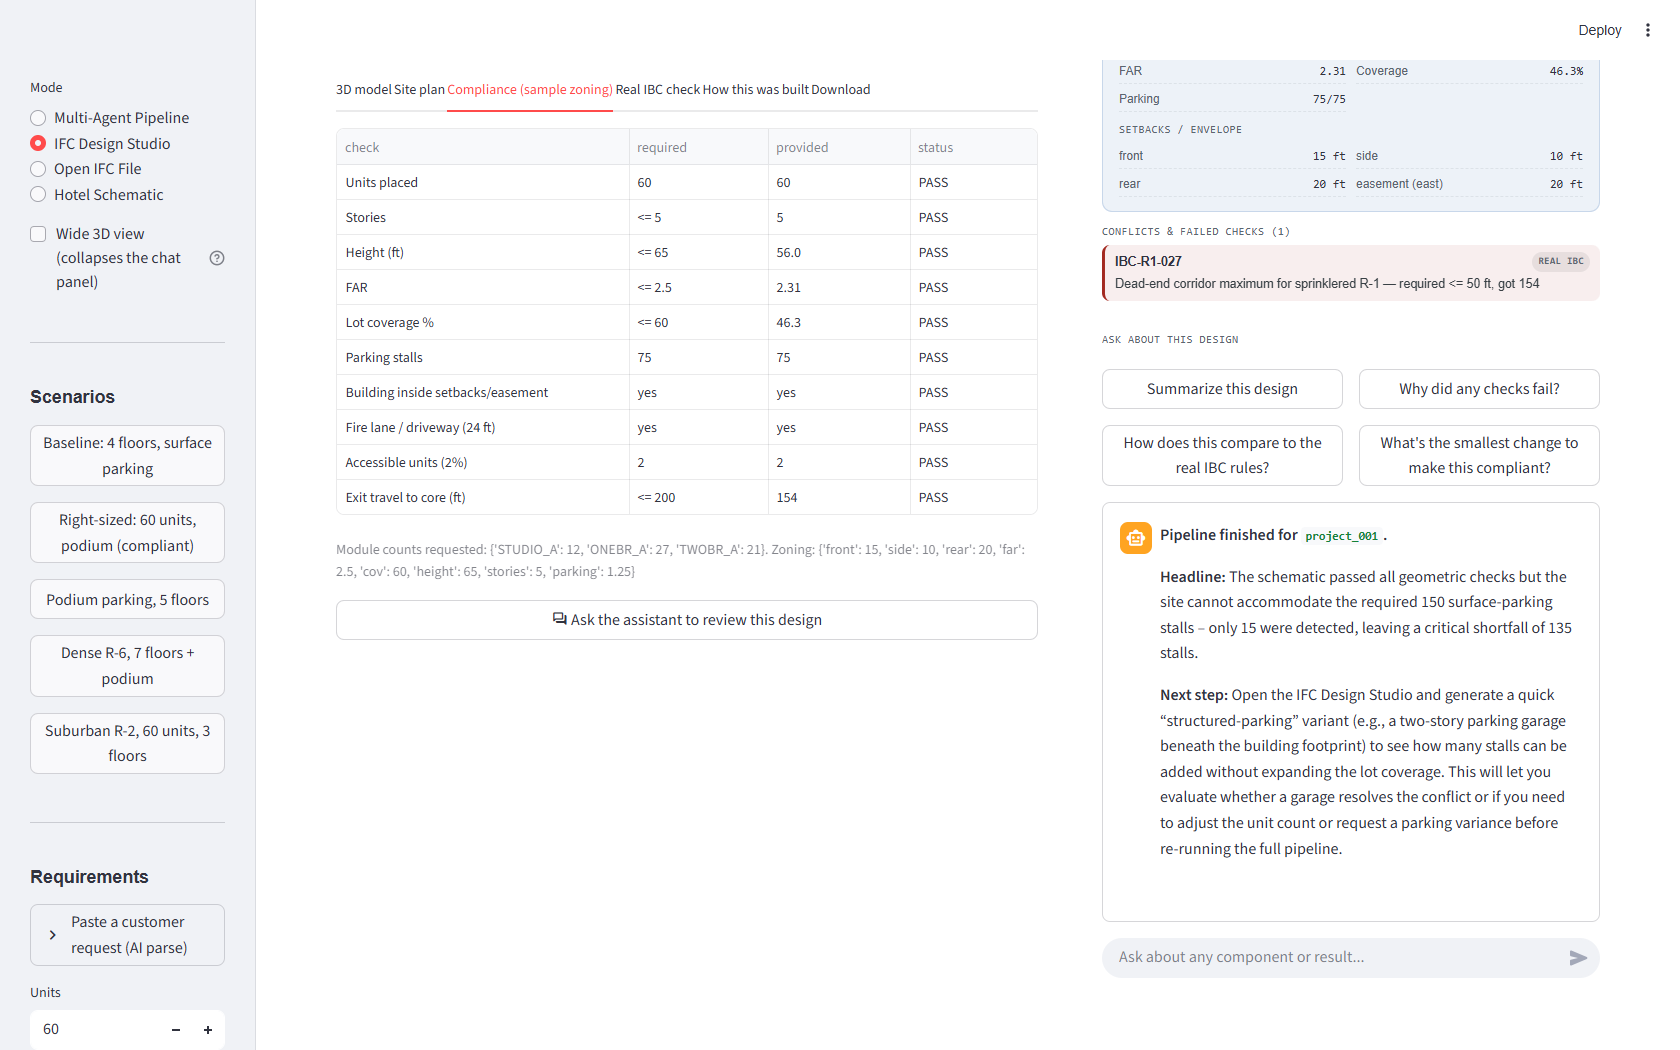
\includegraphics[width=\linewidth,keepaspectratio,height=0.42\textheight]{screens/15_ifc_rightsized_compliance.png}\caption{Right-sized scenario (60 units, podium parking): the compliance checks after the fix.}\end{figure}
\begin{figure}[H]\centering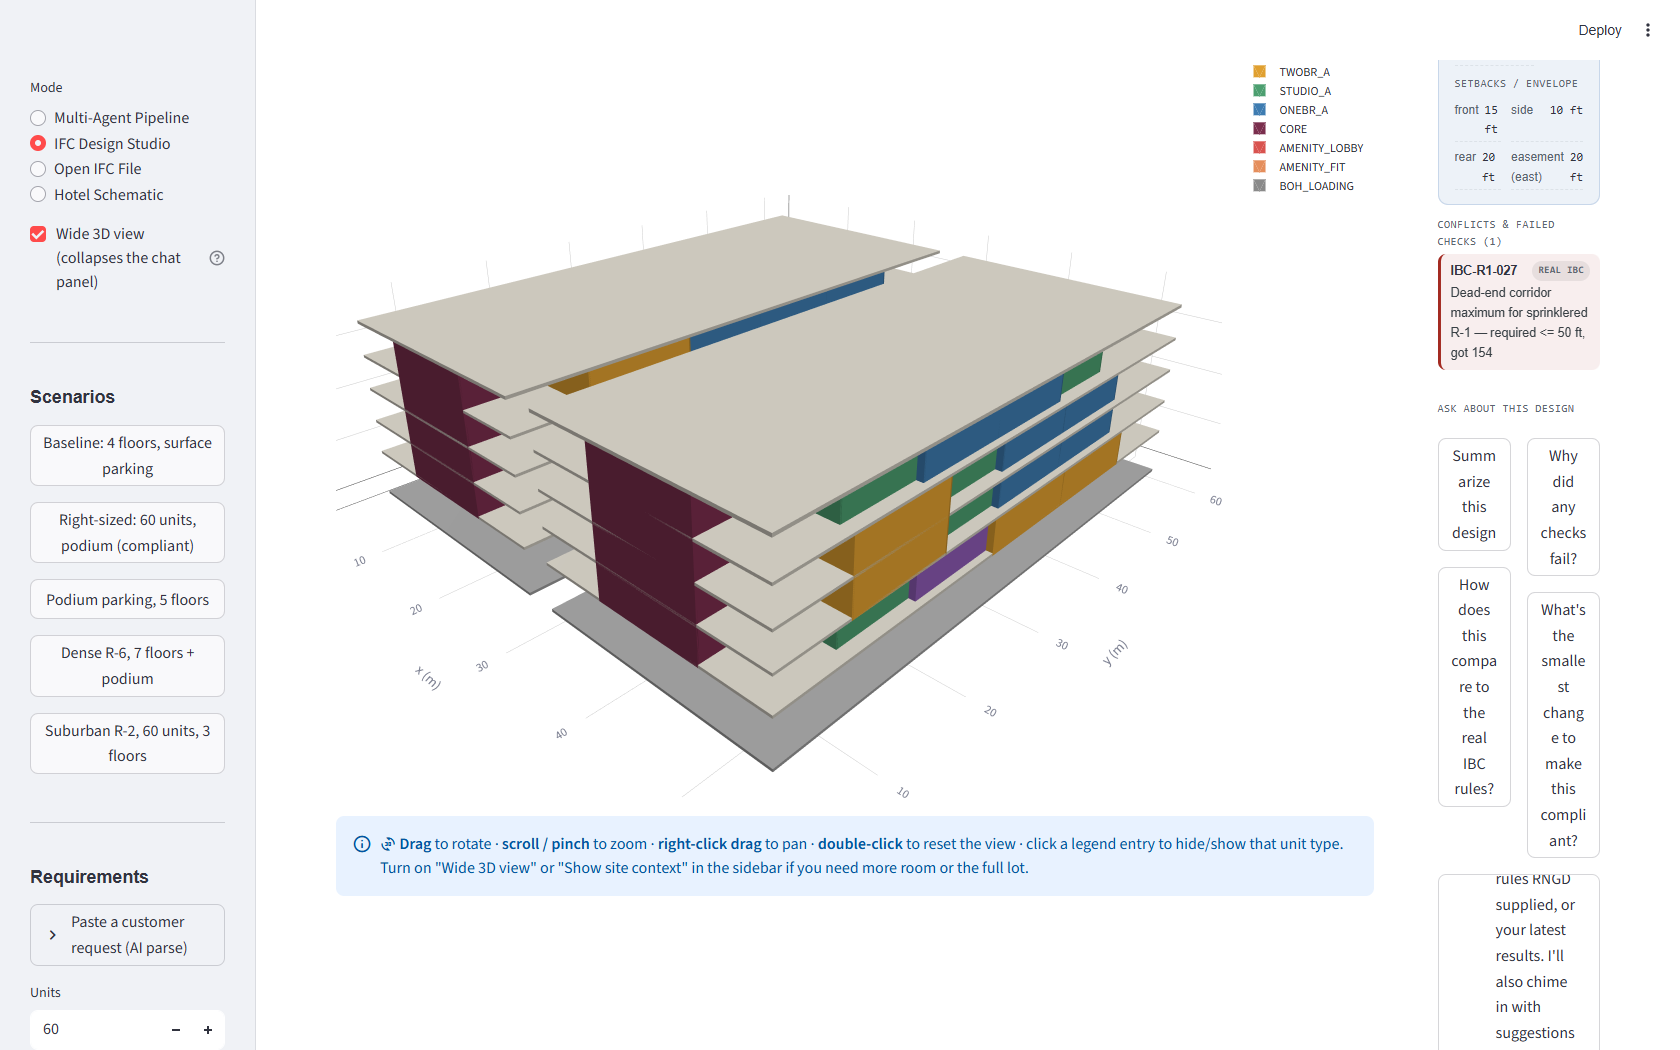
\includegraphics[width=\linewidth,keepaspectratio,height=0.42\textheight]{screens/16_ifc_rightsized_3d.png}\caption{Right-sized scenario in 3D.}\end{figure}


\section{Open IFC File (a real model)}
\subsection{What it does}
Opens an arbitrary real \texttt{.ifc} file, triangulates its geometry, recentres it on the structure (dropping far-away
outliers so the building fills the view) and summarises what is in it. The file used is real, supplied for testing.

\subsection{Result}
{\small \begin{longtable}{p{4.2cm}p{11.8cm}}
\toprule
\textbf{Item} & \textbf{Value} \\ \midrule \endhead
File & CDI SOLUTIONS\_METAIRIE BANK\_R21.ifc (89.4 MB) \\
Schema & IFC2X3 \\
Project & METAIRIE BANK \\
Site / building & Default / None \\
Storeys & FIRST FLOOR (0.0 m), MIDDLE ROOF (14.0 m), HIGH ROOF (16.0 m) \\
IFC elements & 1,537 \\
Meshes triangulated & 881 \\
Building diagonal & 134.8 m \\
Outliers excluded from the view & 4 (e.g. Night DropBox:Night DropBox:6634177 at 896.5 m) \\
\bottomrule
\end{longtable}}
{\small \begin{longtable}{p{7cm}p{3cm}}
\toprule
\textbf{IFC class} & \textbf{Count} \\ \midrule \endhead
IfcMember & 467 \\
IfcBuildingElementProxy & 166 \\
IfcPlate & 148 \\
IfcWall & 144 \\
IfcWallStandardCase & 139 \\
IfcFurnishingElement & 129 \\
IfcFlowTerminal & 128 \\
IfcCurtainWall & 36 \\
IfcSlab & 25 \\
IfcDoor & 23 \\
IfcCovering & 22 \\
IfcWindow & 7 \\
IfcRoof & 2 \\
\bottomrule
\end{longtable}}
Notable named items: Wall Sweep (45), Lighting\_Fixture-PureEdge\_Lighting-Cirrus-D1\_Modular\_Suspension (36), Lighting\_Fixture-PureEdge\_Lighting-Cirrus-D1\_Modular\_Suspension-120\_Connector (36), Lighting\_Fixture-Focal\_Point-Amica\_2x4 (19), National - Grin - Guest chair (16), Lighting\_Fixture-Focal\_Point-Seem\_1\_Recessed\_LED\_FSM1 (15), Recessed Lamp - Round - LED (14), Model Text (11), Roller Window Shades (10), CW Cupbd Ohead (9), Knoll\_Antenna\_Legs\_Table\_Desks (8), Knoll\_Antenna\_Tops\_Rectangular (8).

\subsection{Screenshots}
\begin{figure}[H]\centering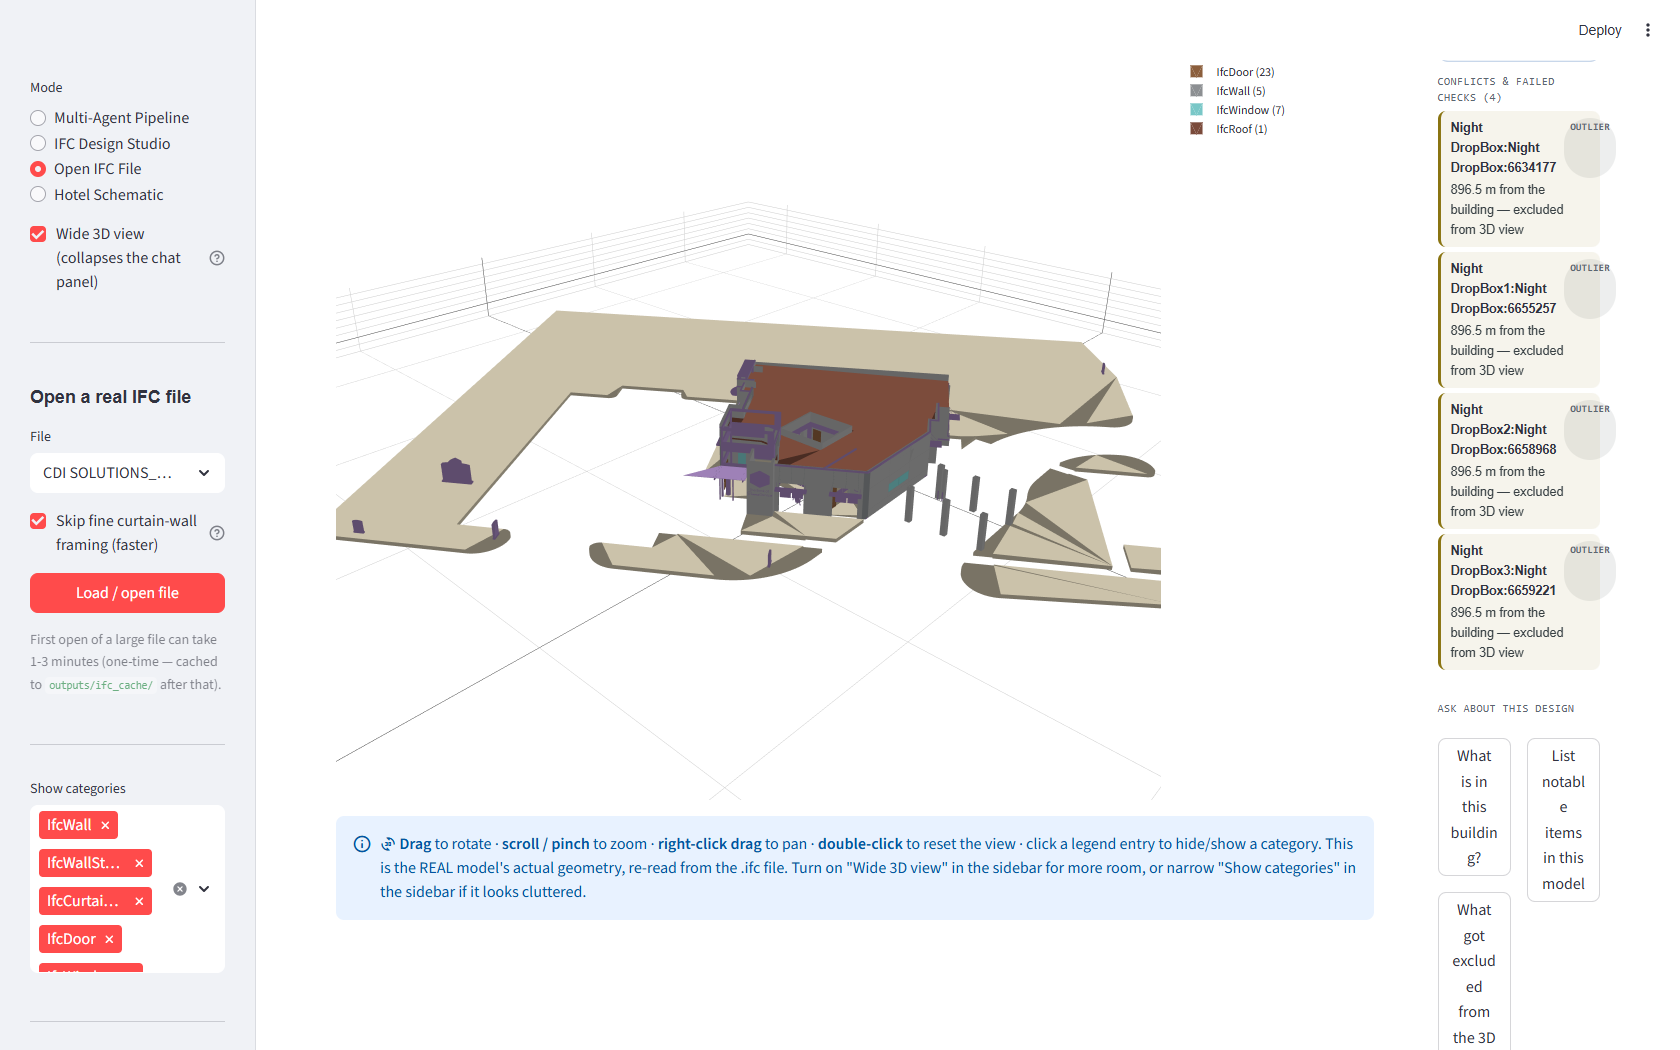
\includegraphics[width=\linewidth,keepaspectratio,height=0.42\textheight]{screens/17_explorer_3d_model.png}\caption{A real IFC file (CDI Solutions, Metairie Bank, IFC2X3, 89 MB) recentred and shown in 3D.}\end{figure}
\begin{figure}[H]\centering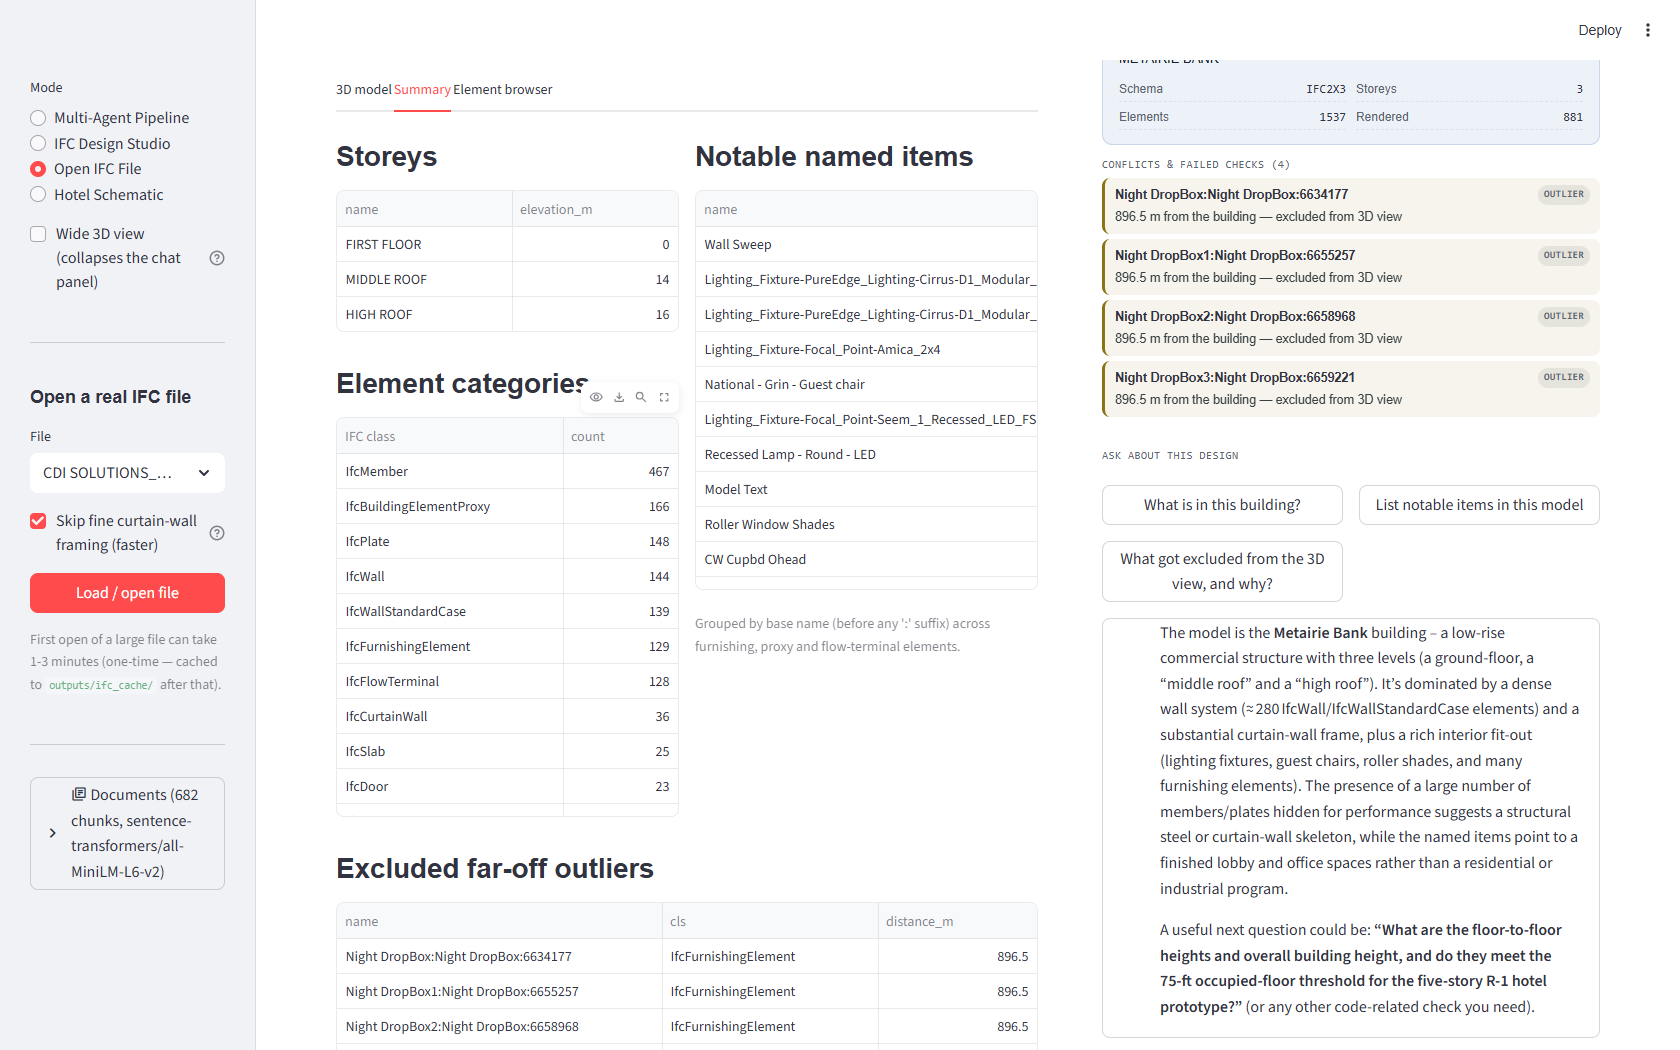
\includegraphics[width=\linewidth,keepaspectratio,height=0.42\textheight]{screens/18_explorer_summary.png}\caption{What is in the real model: schema, storeys and element counts by IFC class.}\end{figure}
\begin{figure}[H]\centering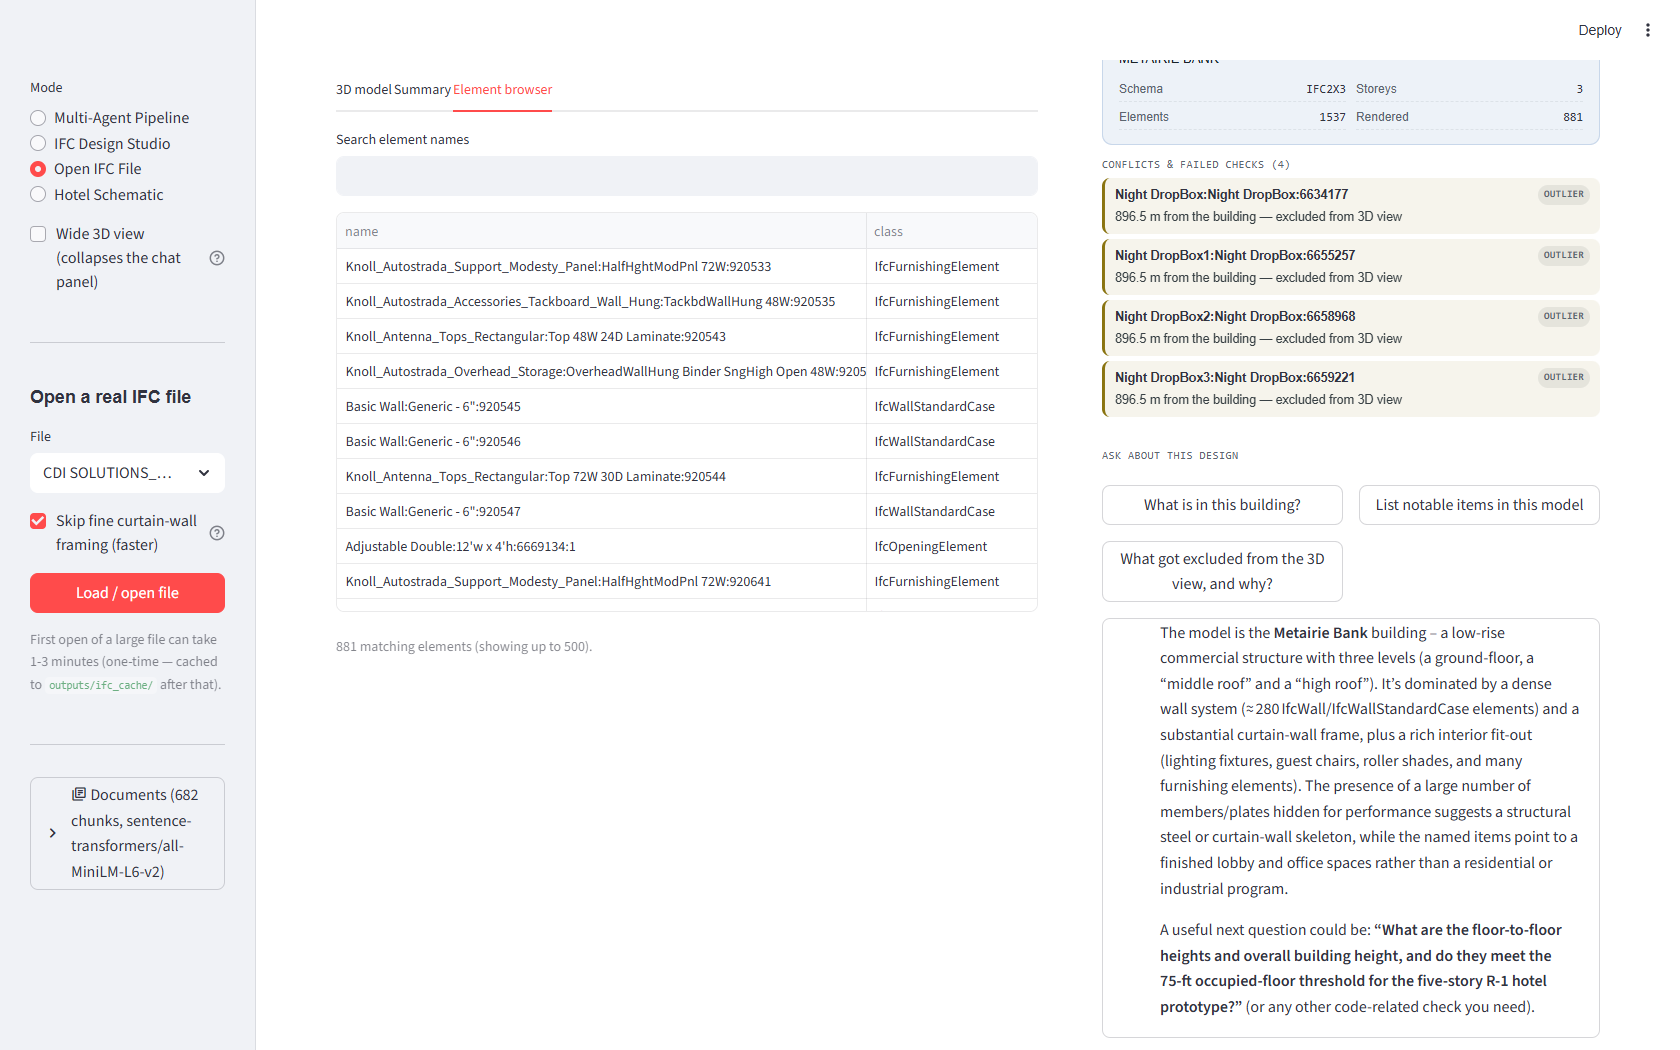
\includegraphics[width=\linewidth,keepaspectratio,height=0.42\textheight]{screens/19_explorer_element_browser.png}\caption{Searchable list of the model's elements.}\end{figure}


\section{Hotel Schematic (RNGD's first use case)}\label{sec:hotel}
\subsection{What it does}
Takes a detailed hotel program --- by default the Project Renegade Living + Lodging cover-sheet space allocation
(28 rows, 117 keys), or an uploaded / in-app edited CSV or XLSX --- and produces a schematic: a Level 1 podium with
lobby, BOH and retail, five double-loaded guest floors with a core and a stair at each end, a code screen against
RNGD's real IBC rule CSV and the 2010 ADA guest-room tables, and an 18 x 12 in drawing set in RNGD's L+L sheet format.

\subsection{Headline results}
\begin{tabular}{p{5cm}p{11cm}}\toprule
Keys & 117 on 5 guest floors \\
Net program area & 59,350 SF (28 rows) \\
Gross area: source sheets / meeting rule / drawn & 74,195 / 85,300 / 76,508 SF \\
Massing & podium 234 x 58 ft, tower 217 x 58 ft, 69.75 ft to roof \\
Code screen & 13 pass, 1 fail, 1 review, 1 assumed \\
Drawing set & 10 sheets, 18 pages, generated 2026-10-05 16:01:06 \\
\bottomrule\end{tabular}

\subsection{Code and ADA screen}
{\small \begin{longtable}{p{1.8cm}p{4.4cm}p{4.4cm}p{3.4cm}p{1.4cm}}
\toprule
\textbf{Rule} & \textbf{Check} & \textbf{Required} & \textbf{Provided} & \textbf{Status} \\ \midrule \endhead
- & Keys placed & 117 & 117 & \textcolor{pass}{\textbf{PASS}} \\
IBC-R1-007 & Stories above grade & $\le$ 5 (Type IIA, sprinklered R-1) & 6 & \textcolor{fail}{\textbf{FAIL}} \\
IBC-R1-005 & Building height (ft) & $\le$ 85 (Type IIA) & 69.8 & \textcolor{pass}{\textbf{PASS}} \\
IBC-R1-010 & Area per story (SF) & $\le$ 72,000 (Type IIA) & 13,575 & \textcolor{pass}{\textbf{PASS}} \\
IBC-R1-012 & High-rise screen (ft to top floor) & $\le$ 75 & 59.0 & \textcolor{pass}{\textbf{PASS}} \\
IBC-R1-015 & Exits per story & 2 for 1-500 occupants & 2 stairs; max load 316 & \textcolor{pass}{\textbf{PASS}} \\
IBC-R1-018 & Exit separation (ft) & $\ge$ 1/3 diagonal = 75 & 207 & \textcolor{pass}{\textbf{PASS}} \\
IBC-R1-023 & Exit access travel (ft) & $\le$ 250 (sprinklered) & 130 & \textcolor{pass}{\textbf{PASS}} \\
IBC-R1-025 & Corridor width (in) & $\ge$ 44 & 72 & \textcolor{pass}{\textbf{PASS}} \\
IBC-R1-027 & Dead-end corridor (ft) & $\le$ 50 (sprinklered R-1) & 5 & \textcolor{pass}{\textbf{PASS}} \\
IBC-R1-028 & Egress door clear width (in) & $\ge$ 32 & 34 (3'-0" leaf) & \textcolor{pass}{\textbf{PASS}} \\
IBC-R1-003 & Automatic sprinklers & NFPA 13 required & assumed & \textcolor{muted}{\textbf{ASSUMED}} \\
ADA-224.2 & Accessible guest rooms (mobility) & $\ge$ 7 for 117 rooms (5 + 2 with roll-in) & 7 & \textcolor{pass}{\textbf{PASS}} \\
ADA-224.4 & Rooms with communication features & $\ge$ 12 & not designated & \textcolor{warn}{\textbf{REVIEW}} \\
ADA-224.5 & Dispersion across room types & spread over 3 types & 3 types: king, suite, two-bed & \textcolor{pass}{\textbf{PASS}} \\
- & Fits buildable envelope & 170 x 265 ft & 234 x 58 ft & \textcolor{pass}{\textbf{PASS}} \\
\bottomrule
\end{longtable}}
\textbf{Notes}\begin{itemize}\item \textbf{IBC-R1-007}: Level 1 counts as a story above grade plane. A Type IA podium (IBC 510.2) could allow 5 stories above it.\item \textbf{IBC-R1-023}: Half the stair-to-stair run plus the room depth.\item \textbf{ADA-224.2}: Confirm which 2 of the ADA units get roll-in showers (Table 224.2).\item \textbf{ADA-224.4}: Designate 12 rooms; at most 10\% of the mobility rooms may count (224.5).\end{itemize}
\textbf{Suggested next steps for the open items}\begin{itemize}\item \textbf{Stories above grade}: Use a Type IA podium for Level 1 (IBC 510.2) so the five guest floors count as a separate building, or drop to four guest floors and lengthen the wing.\item \textbf{Rooms with communication features}: Mark the communication-feature rooms in the program (visual alarms, notification devices).\end{itemize}

\subsection{Levels}
{\small \begin{longtable}{p{2cm}p{2cm}p{2.6cm}p{2.8cm}p{2.8cm}p{1.2cm}}
\toprule
\textbf{Level} & \textbf{Floor at (ft)} & \textbf{Footprint (ft)} & \textbf{Gross drawn (SF)} & \textbf{Gross source (SF)} & \textbf{Keys} \\ \midrule \endhead
Level 1 & 0.00 & 234 x 58 & 13,575 & 12,485 & 0 \\
Level 2 & 16.00 & 217 x 58 & 12,587 & 12,342 & 24 \\
Level 3 & 26.75 & 217 x 58 & 12,587 & 12,342 & 24 \\
Level 4 & 37.50 & 217 x 58 & 12,587 & 12,342 & 23 \\
Level 5 & 48.25 & 217 x 58 & 12,587 & 12,342 & 23 \\
Level 6 & 59.00 & 217 x 58 & 12,587 & 12,342 & 23 \\
\bottomrule
\end{longtable}}

\subsection{Detailed program}
{\small \begin{longtable}{p{1.4cm}p{3.0cm}p{0.8cm}p{1.0cm}p{1.1cm}p{1.6cm}p{1.6cm}p{0.9cm}p{2.2cm}p{0.7cm}}
\toprule
\textbf{Group} & \textbf{Type} & \textbf{Count} & \textbf{Each SF} & \textbf{Total SF} & \textbf{Size} & \textbf{Beds} & \textbf{Sleeps} & \textbf{Placed on} & \textbf{Occ.} \\ \midrule \endhead
Shared & Corridor & 1 & 1,335 & 1,335 &  &  &  & L1, L2, L3, L4, L5, L6 &  \\
Shared & Gym & 1 & 968 & 968 &  &  &  & L1 & 20 \\
Shared & Lobby & 1 & 2,865 & 2,865 &  &  &  & L1 & 191 \\
Shared & Mens & 1 & 205 & 205 &  &  &  & L1 &  \\
Shared & Womens & 1 & 200 & 200 &  &  &  & L1 &  \\
BOH & BOH & 1 & 69 & 69 &  &  &  & L1 & 1 \\
BOH & Hotel Kitchen / Pantry & 1 & 331 & 331 &  &  &  & L1 & 2 \\
BOH & Housekeeping & 1 & 103 & 103 &  &  &  & L1 & 1 \\
BOH & Ice & 5 & 59 & 297 &  &  &  & every guest floor & 1 \\
BOH & IT & 5 & 74 & 372 &  &  &  & every guest floor & 2 \\
BOH & Jan & 5 & 54 & 269 &  &  &  & every guest floor & 1 \\
BOH & Janitor & 1 & 107 & 107 &  &  &  & L1 & 1 \\
BOH & Loading & 1 & 282 & 282 &  &  &  & L1 & 1 \\
BOH & MEP Service & 1 & 309 & 309 &  &  &  & L1 & 2 \\
BOH & Stair & 12 & 156 & 1,868 &  &  &  & 2 per level (stacked) &  \\
BOH & Supplies & 5 & 79 & 394 &  &  &  & every guest floor & 2 \\
Tenant & White Box Retail & 1 & 3,533 & 3,533 &  &  &  & L1 & 59 \\
Hotel Units & ADA Corner Suite & 1 & 852 & 852 & 32.8' x 26' & 1 king + sofa & 4 & L4 & 5 \\
Hotel Units & ADA King Spa & 2 & 460 & 920 & 17.7' x 26' & 1 king & 4 & L5, L6 & 5 \\
Hotel Units & ADA QQ & 2 & 446 & 892 & 17.2' x 26' & 2 queens & 8 & L5, L6 & 5 \\
Hotel Units & ADA Suite & 2 & 639 & 1,278 & 24.6' x 26' & 1 king + sofa & 8 & L3, L4 & 7 \\
Hotel Units & Corner Suite & 2 & 864 & 1,728 & 33.2' x 26' & 1 king + sofa & 8 & L2, L3 & 9 \\
Hotel Units & King & 69 & 343 & 23,692 & 13.2' x 26' & 1 king & 138 & every guest floor & 119 \\
Hotel Units & King Spa & 3 & 460 & 1,379 & 17.7' x 26' & 1 king & 6 & L2, L3, L4 & 7 \\
Hotel Units & QQ & 33 & 344 & 11,342 & 13.2' x 26' & 2 queens & 132 & every guest floor & 57 \\
Hotel Units & Suite & 3 & 640 & 1,920 & 24.6' x 26' & 1 king + sofa & 12 & L2, L5, L6 & 10 \\
Business & BOH / Bus & 1 & 1,718 & 1,718 &  &  &  & L1 & 12 \\
Business & Luggage & 1 & 122 & 122 &  &  &  & L1 & 1 \\
\bottomrule
\end{longtable}}

\subsection{Room mix by floor}
{\small \begin{longtable}{p{3.4cm}p{1.5cm}p{1.5cm}p{1.5cm}p{1.5cm}p{1.5cm}p{1.5cm}}
\toprule
\textbf{Type} & \textbf{Level 2} & \textbf{Level 3} & \textbf{Level 4} & \textbf{Level 5} & \textbf{Level 6} & \textbf{Total} \\ \midrule \endhead
Corner Suite & 1 & 1 & 0 & 0 & 0 & 2 \\
King Spa & 1 & 1 & 1 & 0 & 0 & 3 \\
QQ & 7 & 7 & 7 & 6 & 6 & 33 \\
King & 14 & 14 & 13 & 14 & 14 & 69 \\
Suite & 1 & 0 & 0 & 1 & 1 & 3 \\
ADA Suite & 0 & 1 & 1 & 0 & 0 & 2 \\
ADA Corner Suite & 0 & 0 & 1 & 0 & 0 & 1 \\
ADA QQ & 0 & 0 & 0 & 1 & 1 & 2 \\
ADA King Spa & 0 & 0 & 0 & 1 & 1 & 2 \\
Keys per floor & 24 & 24 & 23 & 23 & 23 & 117 \\
\bottomrule
\end{longtable}}

\subsection{App screenshots}
\begin{figure}[H]\centering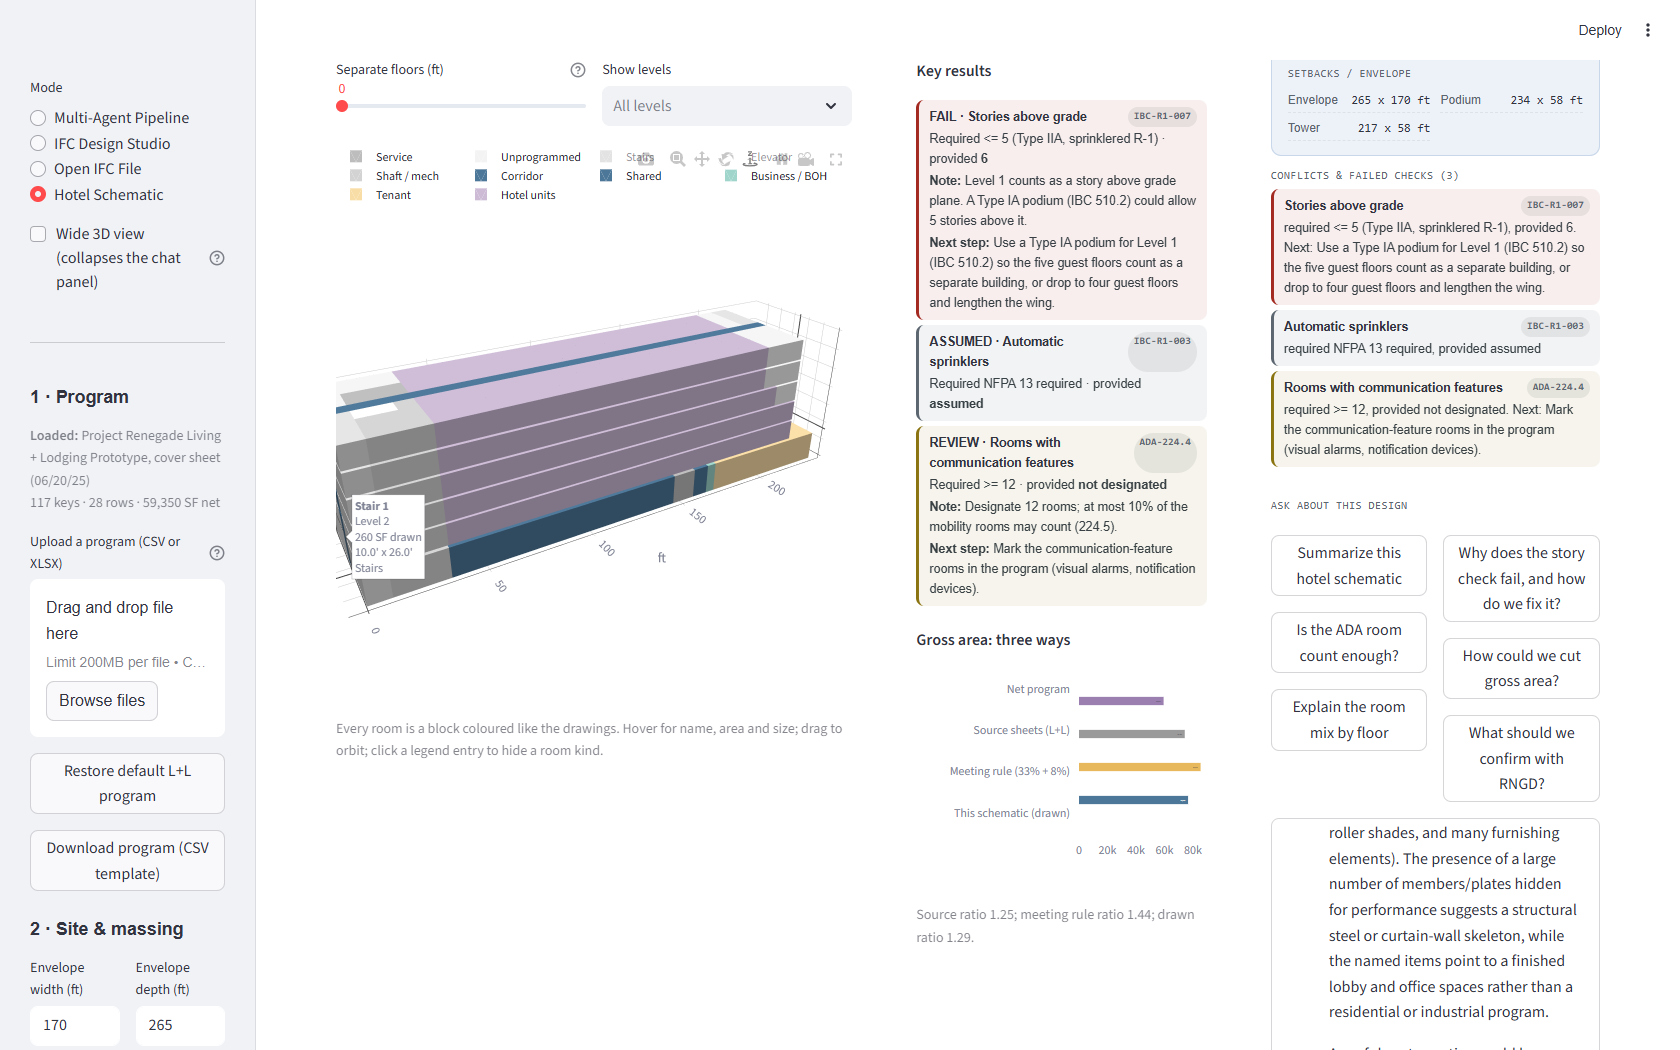
\includegraphics[width=\linewidth,keepaspectratio,height=0.42\textheight]{screens/20_hotel_overview.png}\caption{Hotel Schematic workspace: KPI tiles, the room-by-room 3D model and the key results with suggested fixes.}\end{figure}
\begin{figure}[H]\centering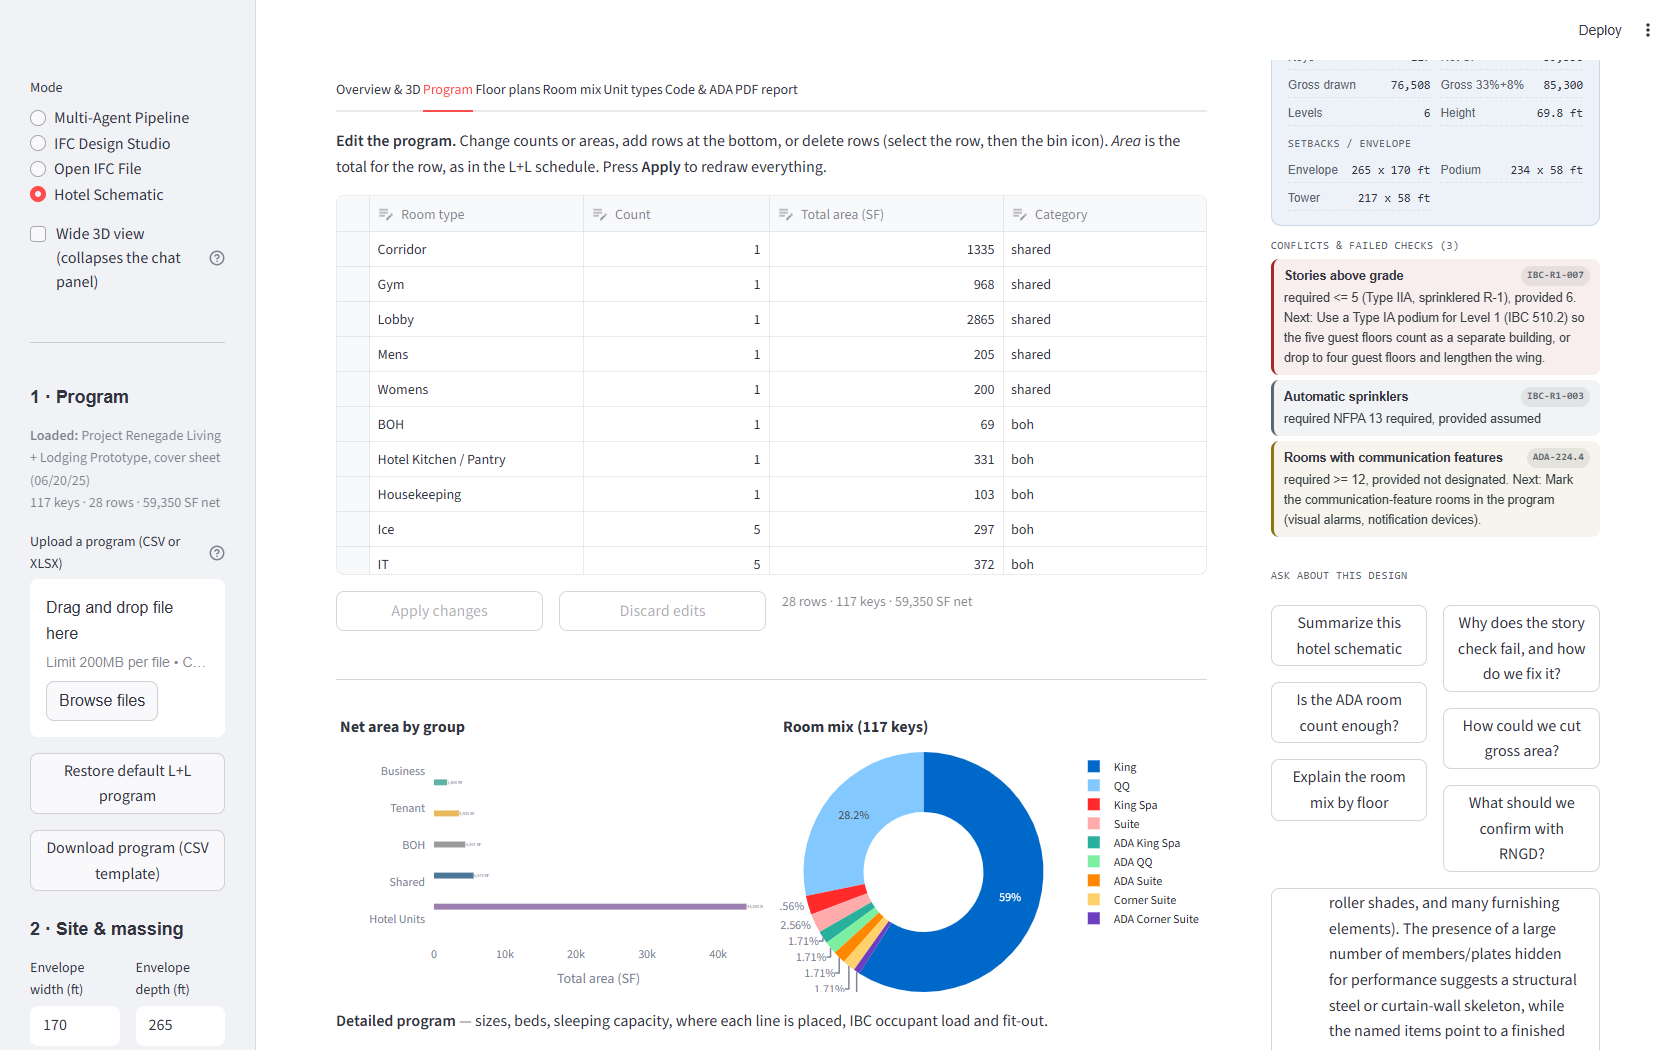
\includegraphics[width=\linewidth,keepaspectratio,height=0.42\textheight]{screens/21_hotel_program.png}\caption{The editable program (Project Renegade L+L space allocation, 28 rows) with area and room-mix charts.}\end{figure}
\begin{figure}[H]\centering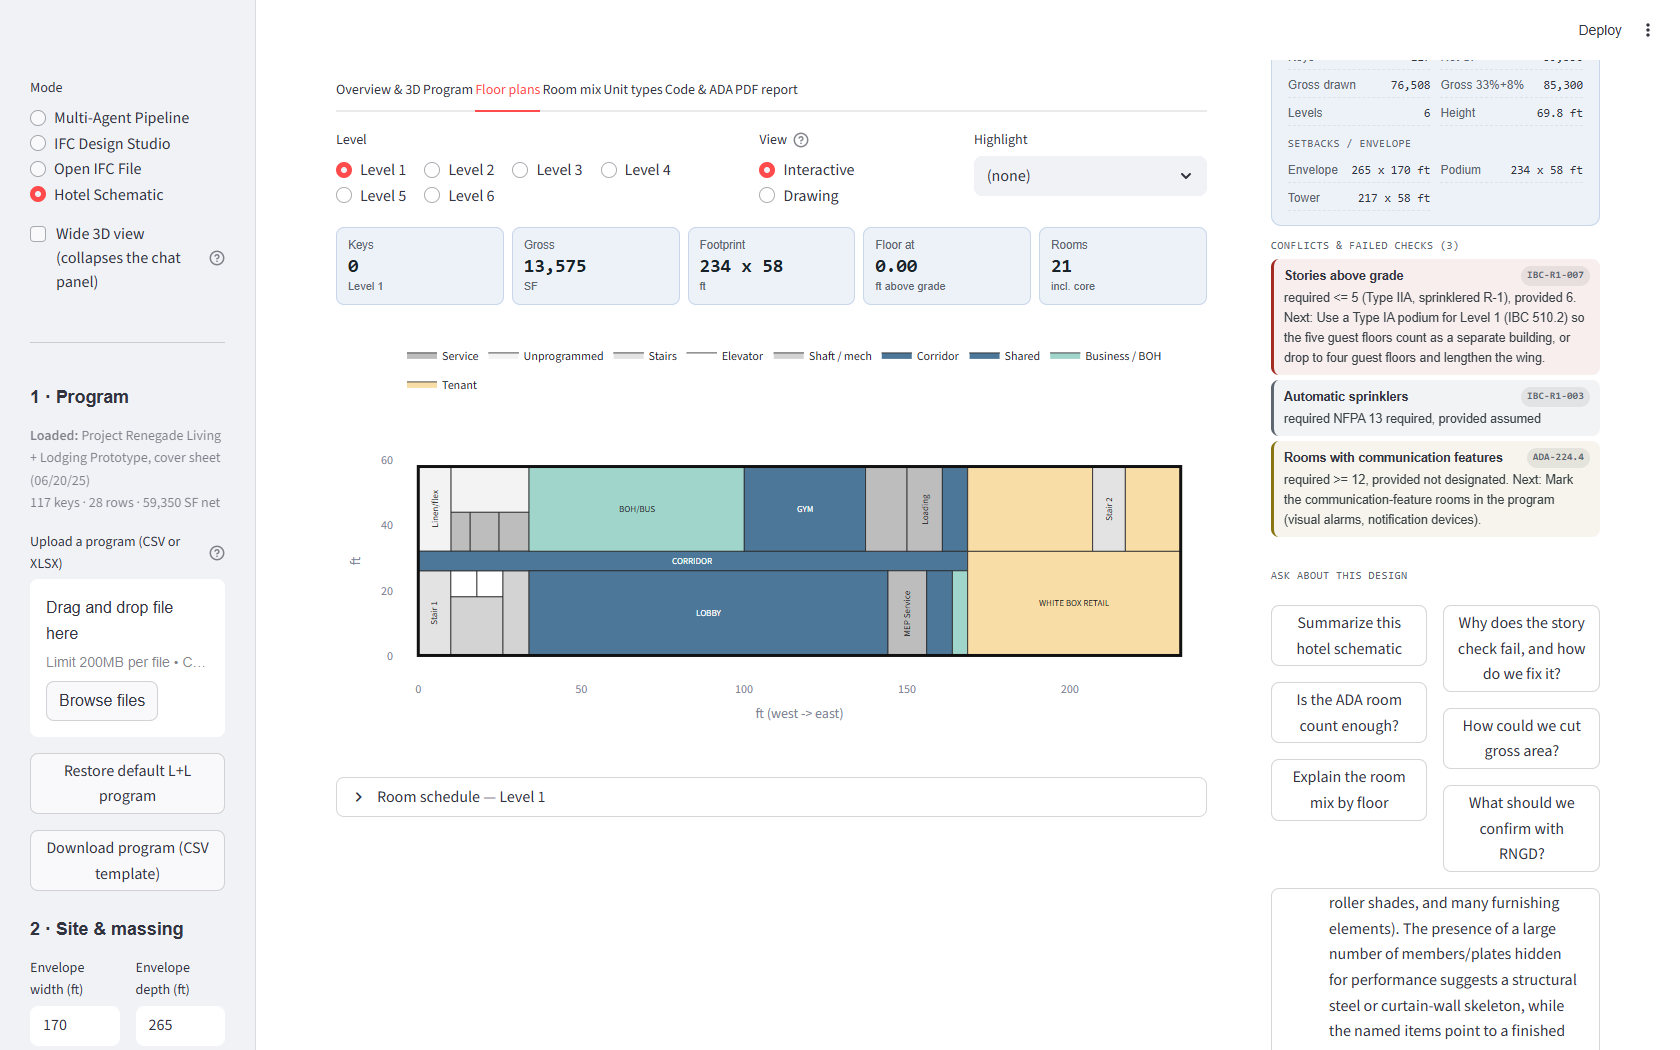
\includegraphics[width=\linewidth,keepaspectratio,height=0.42\textheight]{screens/22_hotel_floor.png}\caption{Interactive floor plan of Level 1 (hover shows each room's area and size).}\end{figure}
\begin{figure}[H]\centering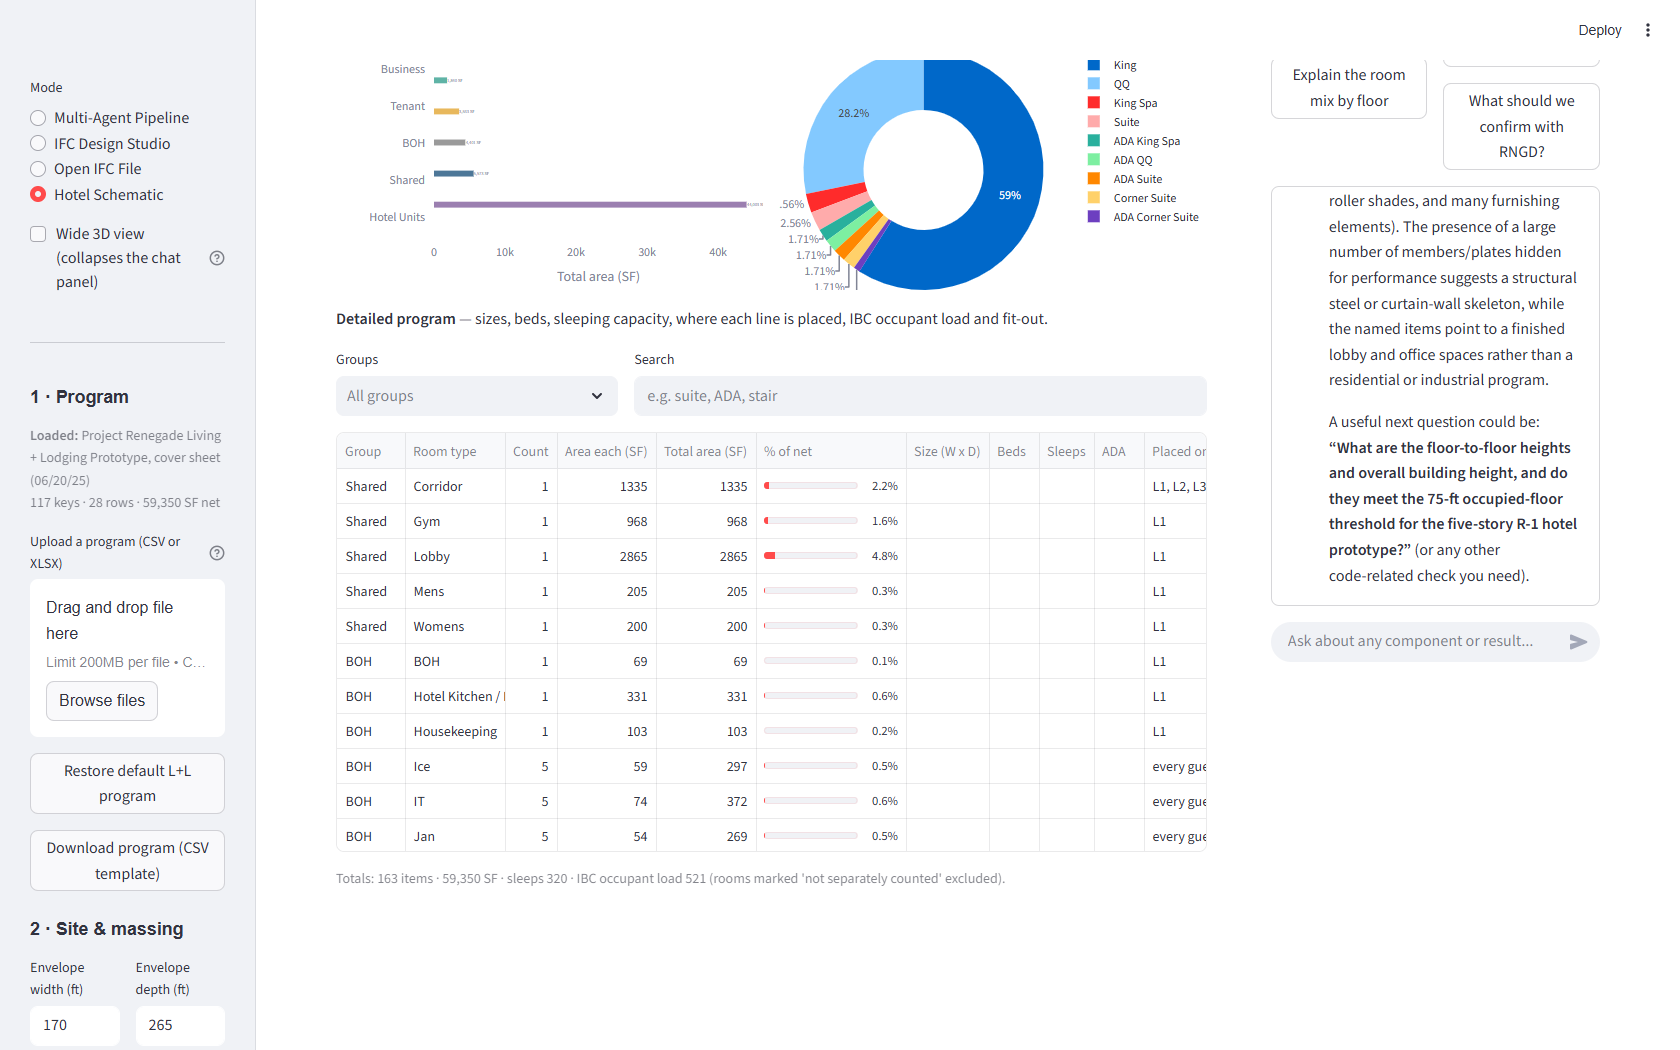
\includegraphics[width=\linewidth,keepaspectratio,height=0.42\textheight]{screens/23_hotel_program_detail.png}\caption{Detailed program: per-room size, beds, sleeping capacity, placement, IBC occupant load and fit-out.}\end{figure}
\begin{figure}[H]\centering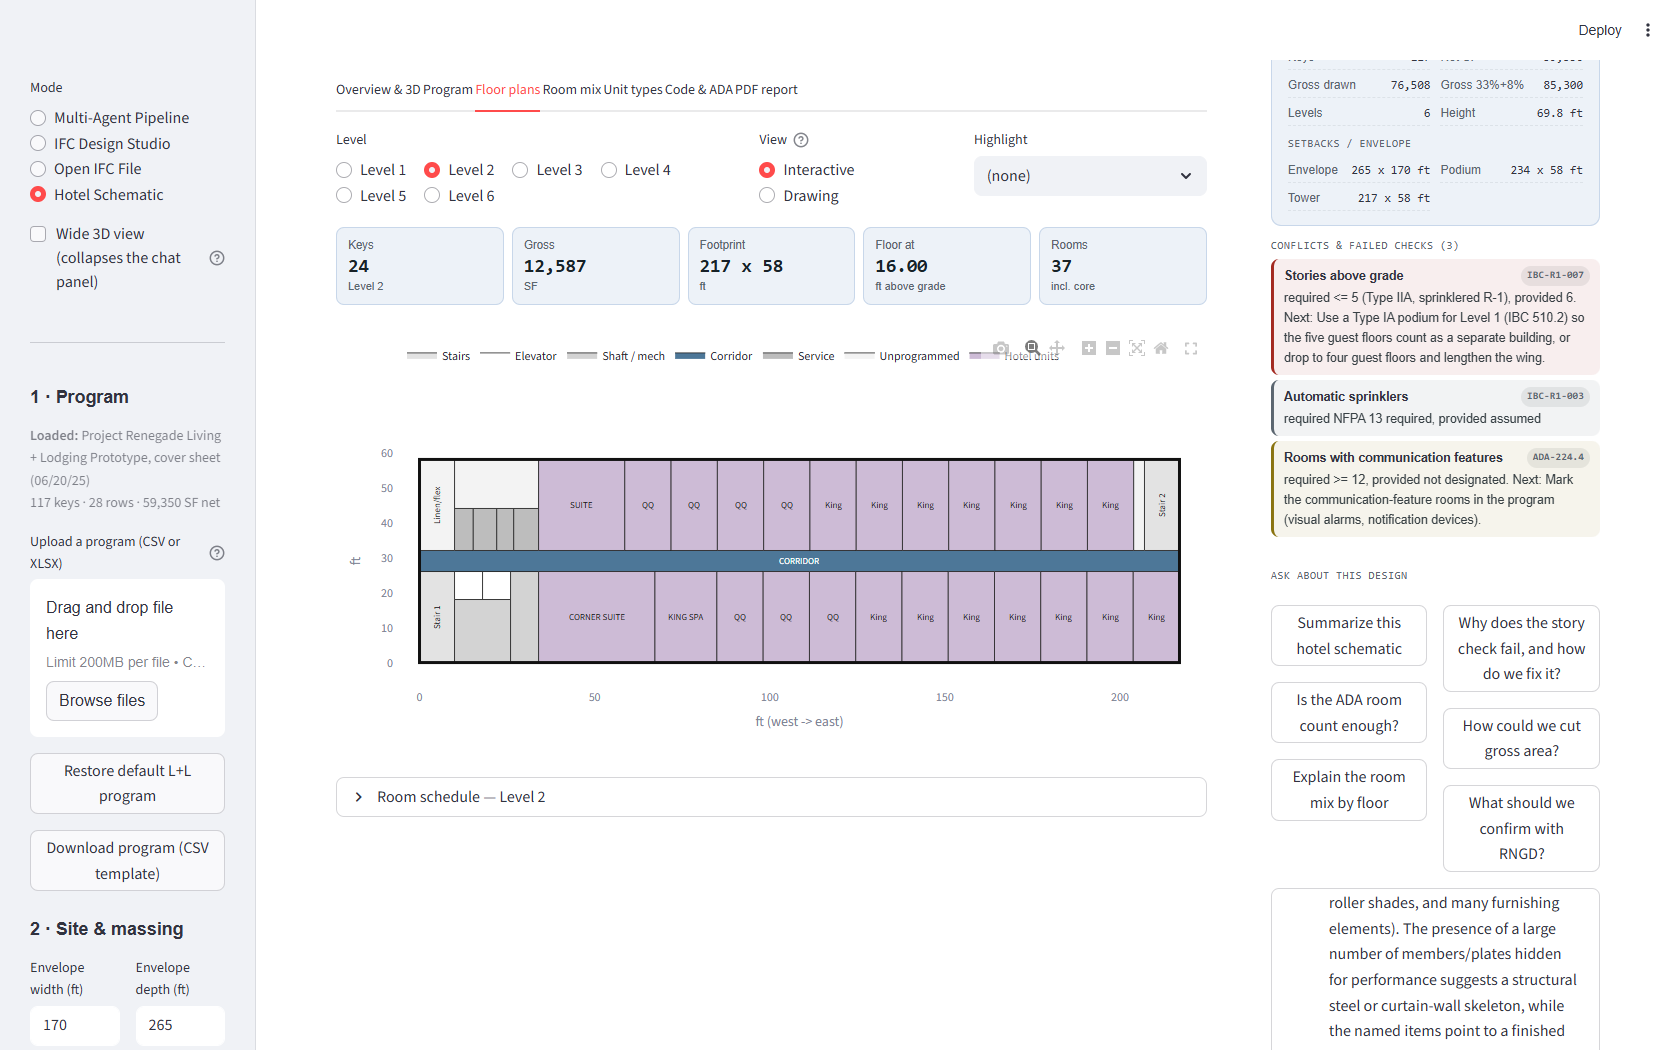
\includegraphics[width=\linewidth,keepaspectratio,height=0.42\textheight]{screens/24_hotel_plan_level2.png}\caption{Interactive plan of Level 2, a typical guest floor (24 keys).}\end{figure}
\begin{figure}[H]\centering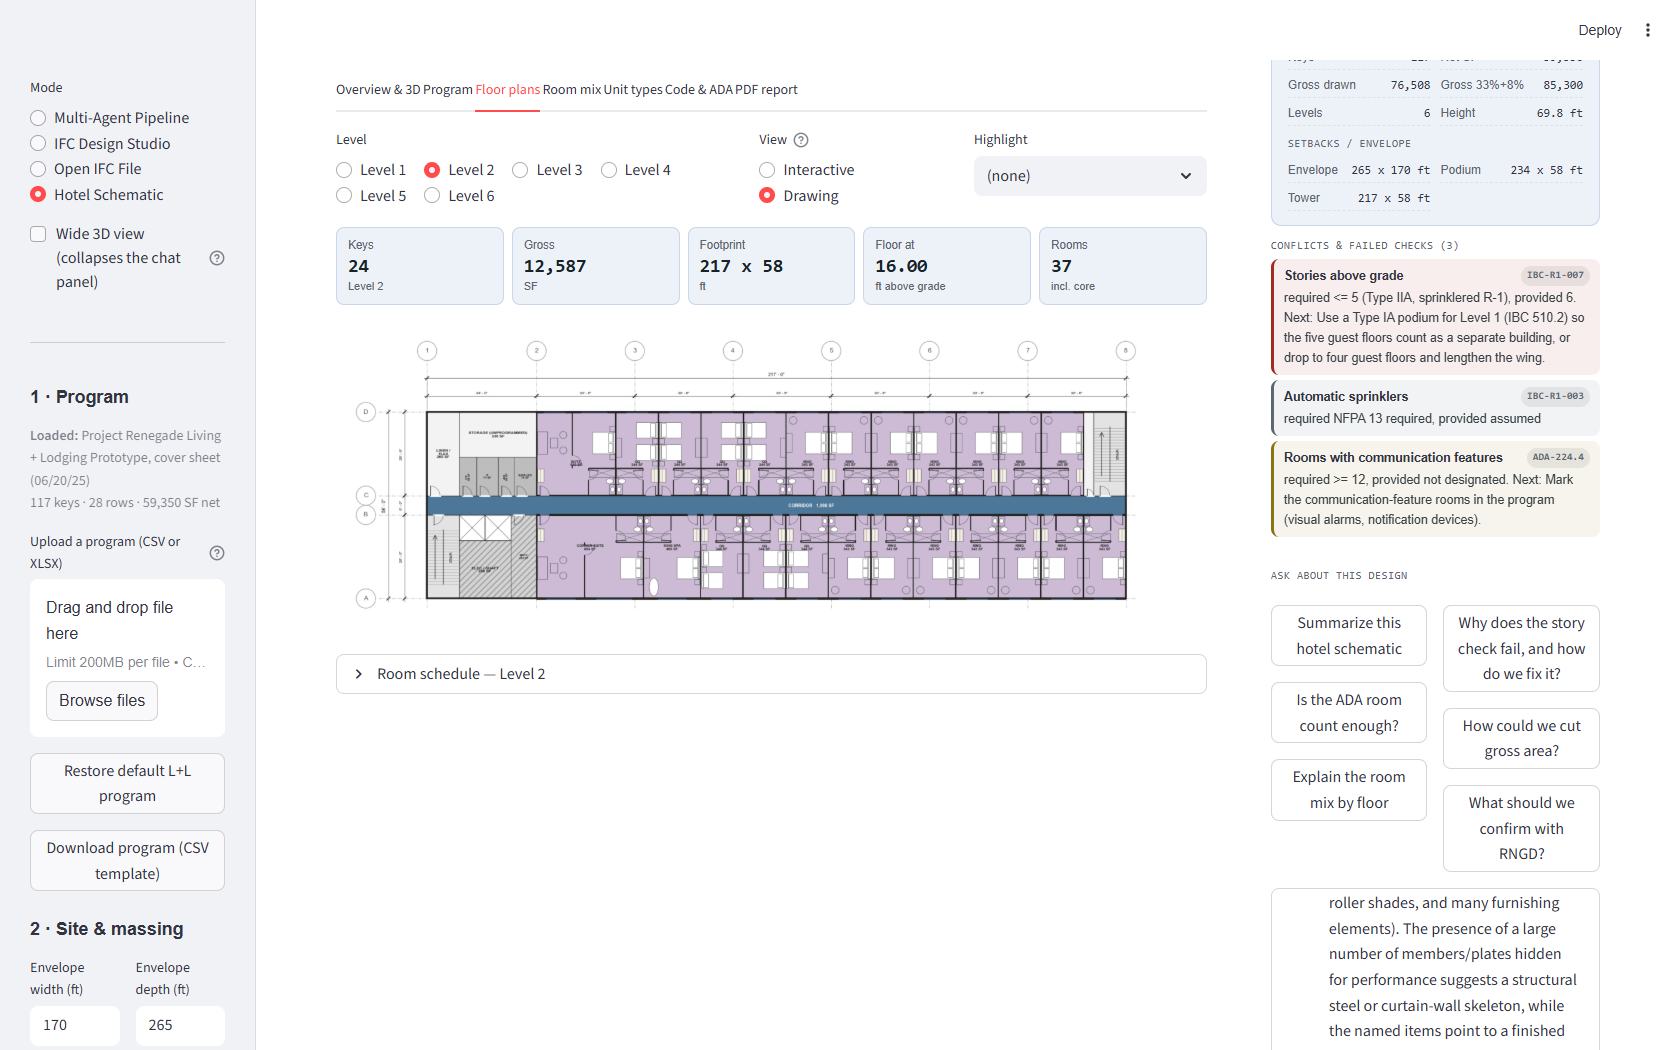
\includegraphics[width=\linewidth,keepaspectratio,height=0.42\textheight]{screens/25_hotel_plan_drawing.png}\caption{The same level in drawing style (as used on the PDF sheets).}\end{figure}
\begin{figure}[H]\centering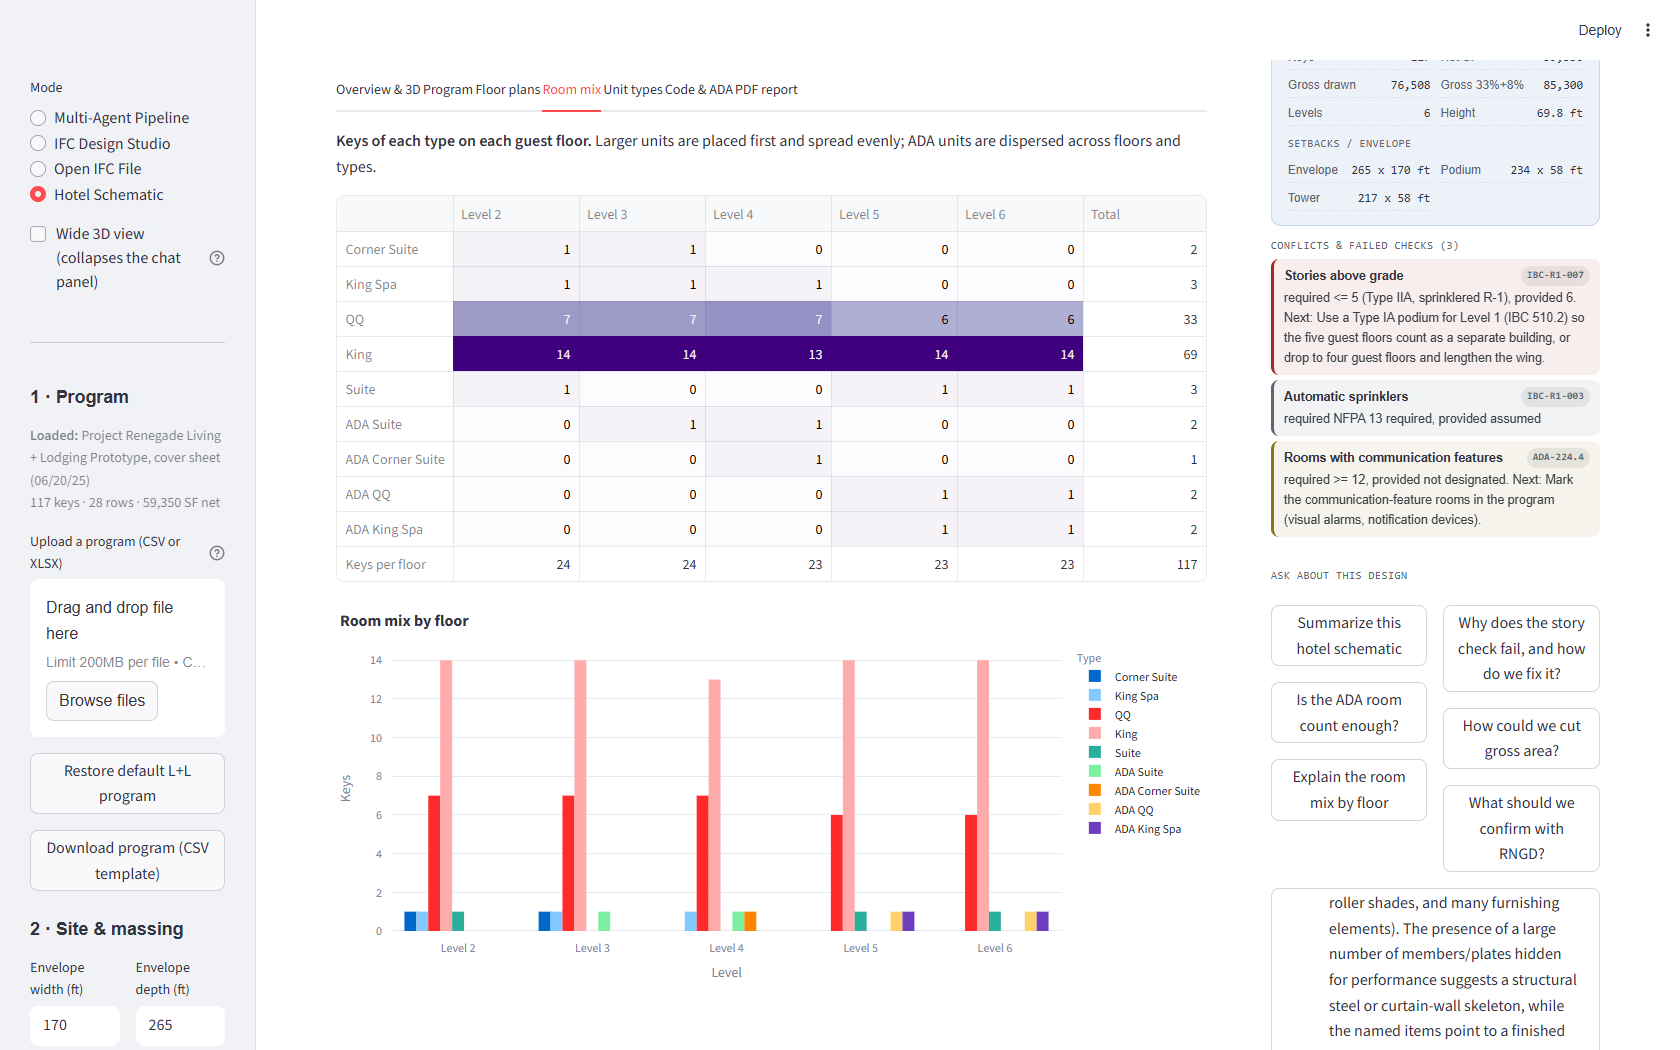
\includegraphics[width=\linewidth,keepaspectratio,height=0.42\textheight]{screens/26_hotel_room.png}\caption{Keys of each room type on each guest floor.}\end{figure}
\begin{figure}[H]\centering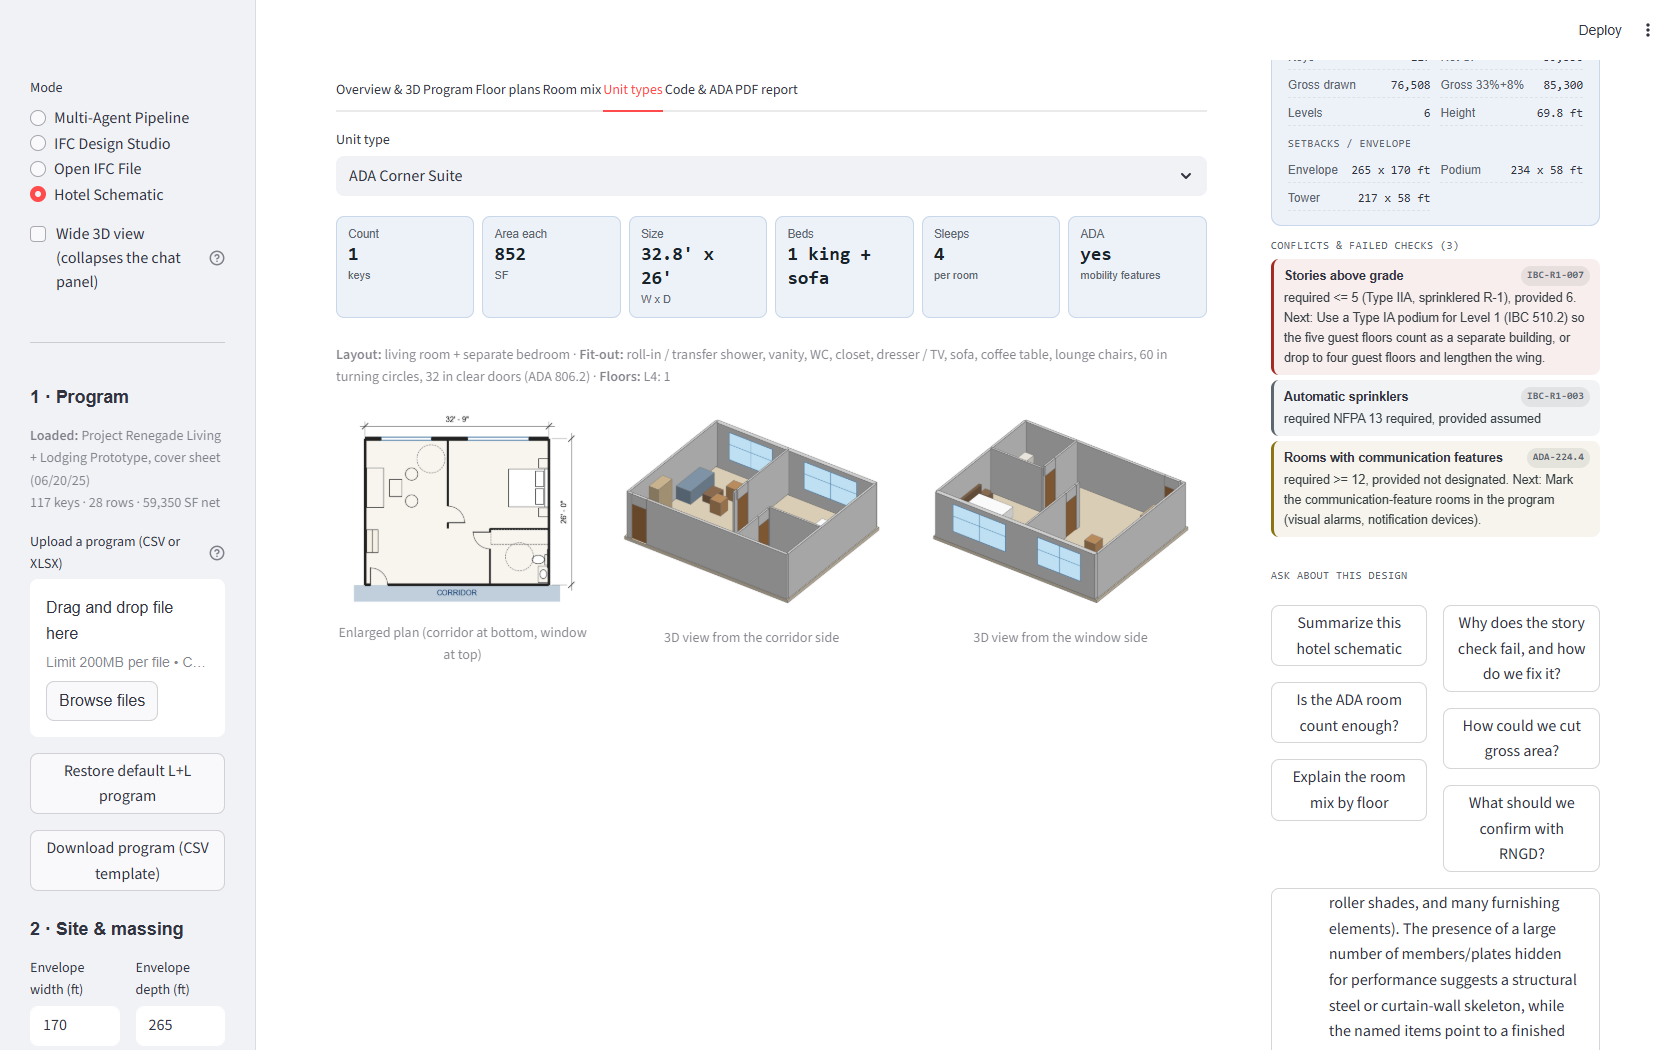
\includegraphics[width=\linewidth,keepaspectratio,height=0.42\textheight]{screens/27_hotel_unit.png}\caption{Unit type detail: enlarged plan and two 3D interior views.}\end{figure}
\begin{figure}[H]\centering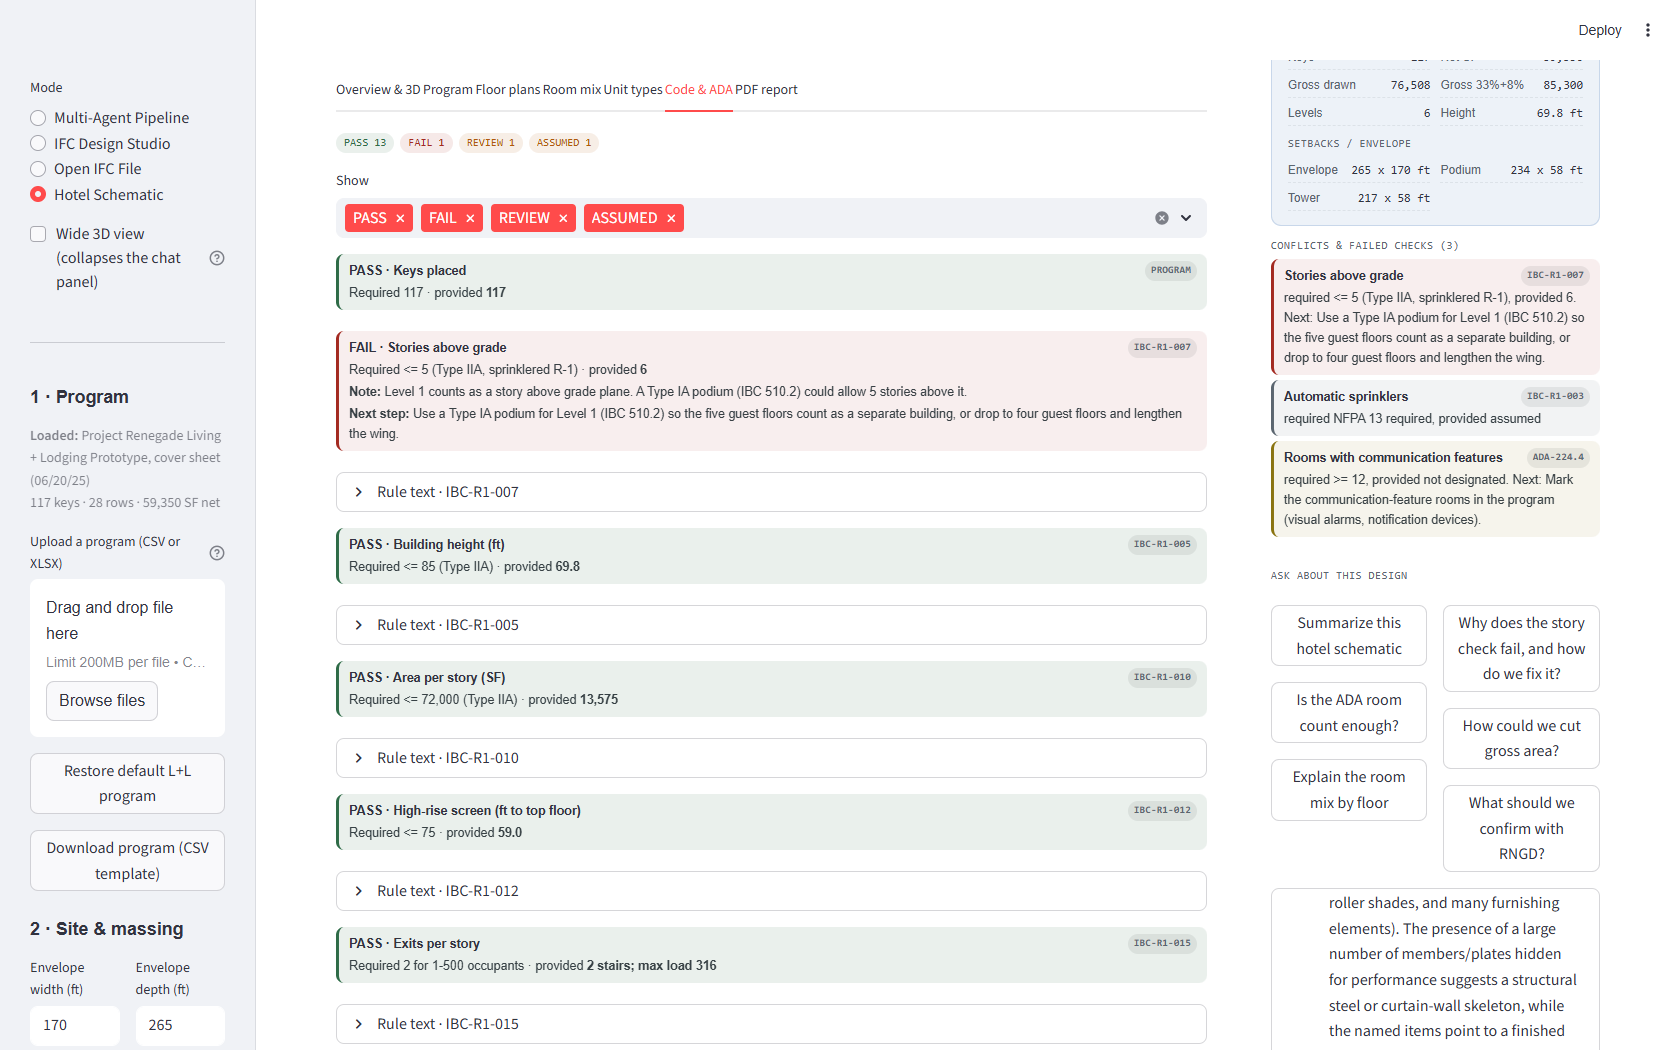
\includegraphics[width=\linewidth,keepaspectratio,height=0.42\textheight]{screens/28_hotel_code.png}\caption{Code screen against RNGD's IBC rule set and the 2010 ADA guest-room tables, with rule text.}\end{figure}
\begin{figure}[H]\centering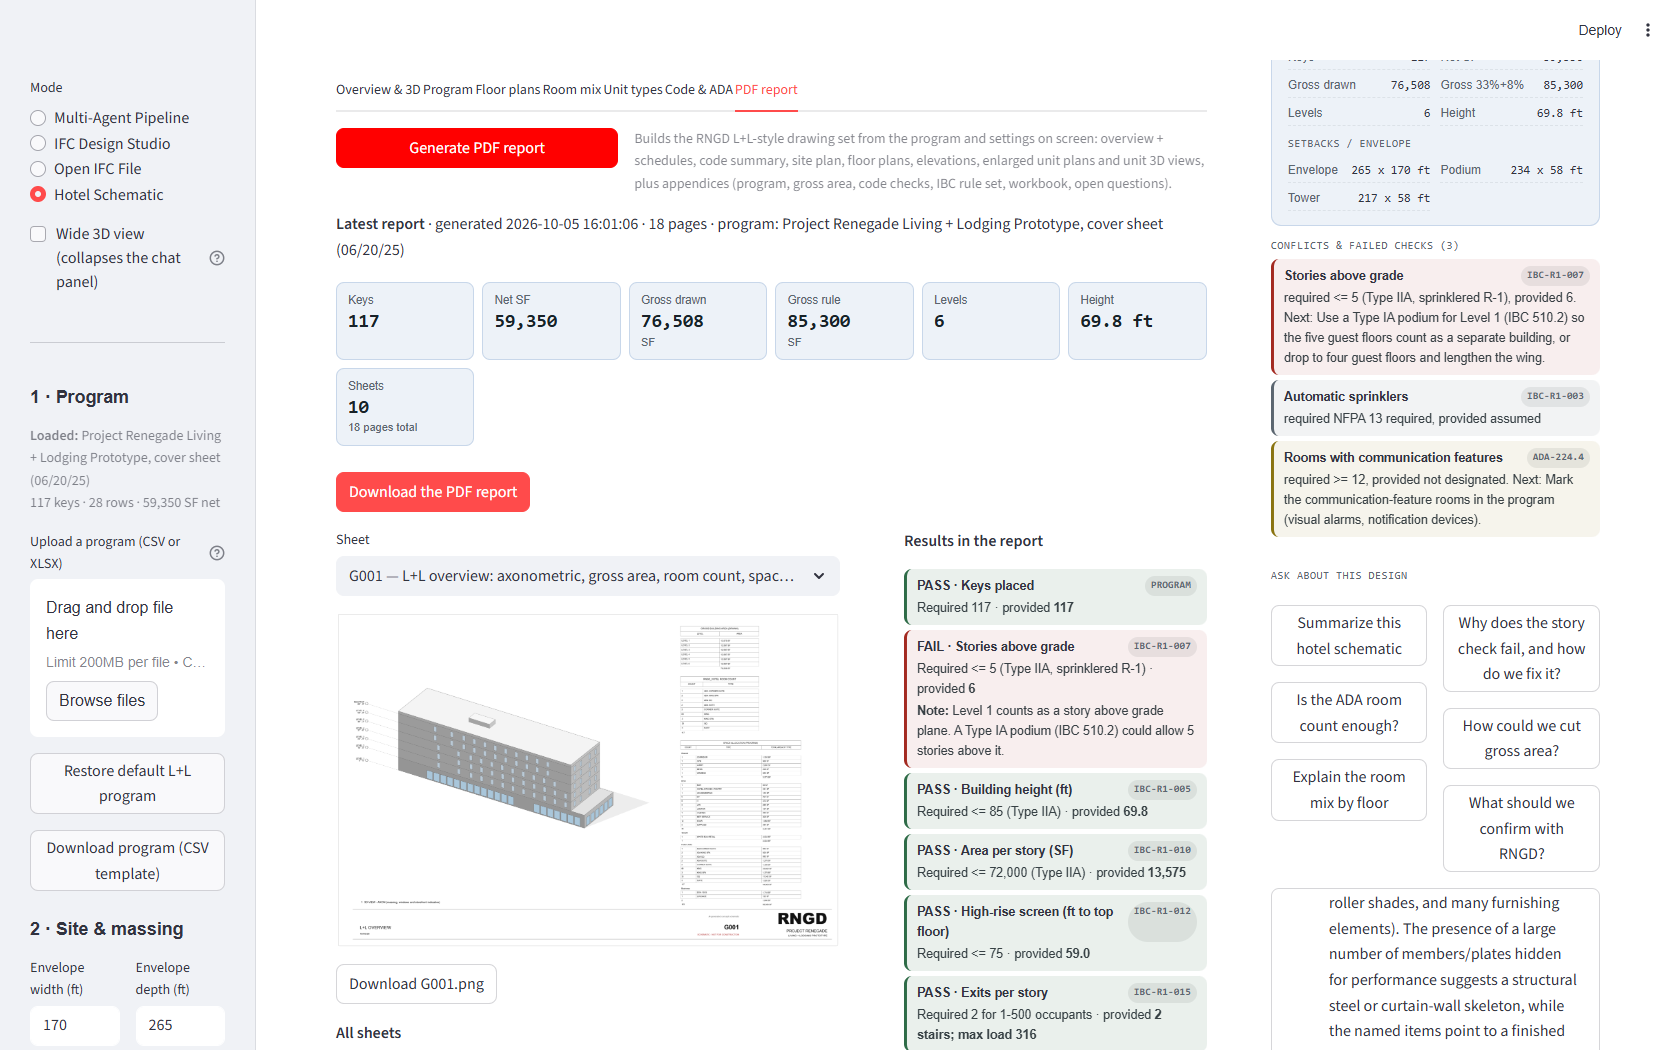
\includegraphics[width=\linewidth,keepaspectratio,height=0.42\textheight]{screens/29_hotel_report_results.png}\caption{PDF report tab after generating: summary numbers and the results that went into the report.}\end{figure}
\begin{figure}[H]\centering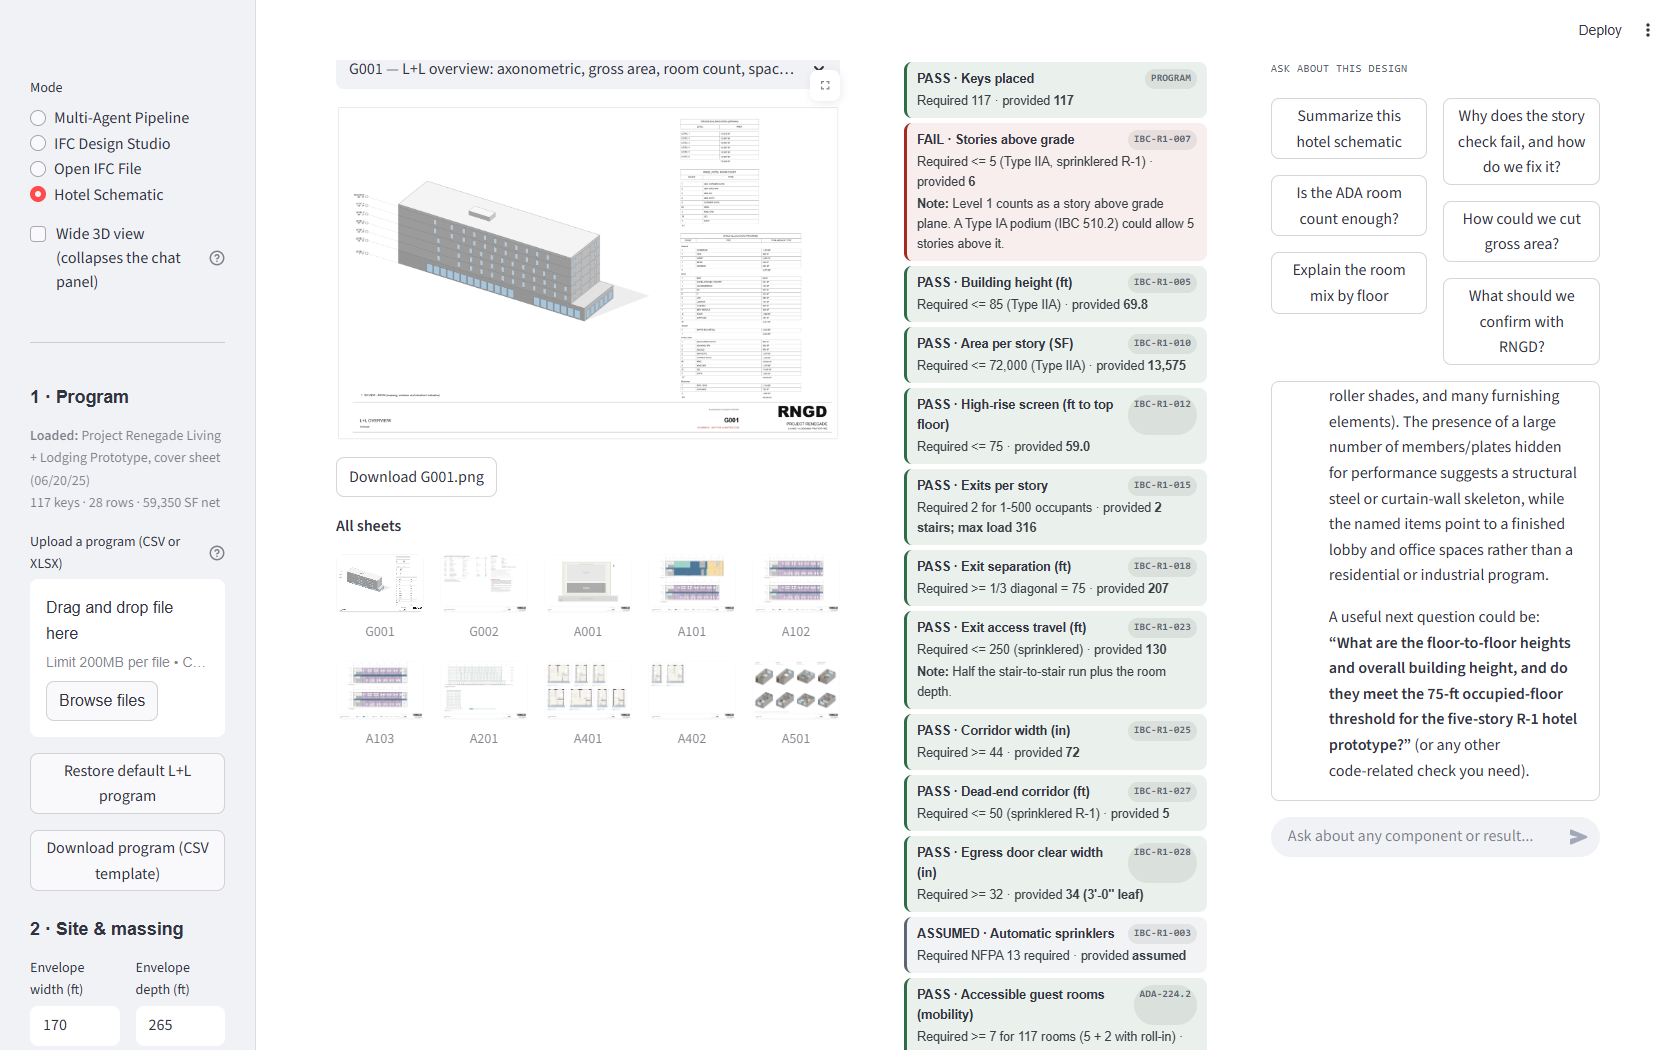
\includegraphics[width=\linewidth,keepaspectratio,height=0.42\textheight]{screens/30_hotel_report_sheets.png}\caption{Sheet gallery of the generated drawing set.}\end{figure}

\subsection{Generated drawing set}
The PDF report (\texttt{reports/final/RNGD\_final\_schematic\_report.pdf}) contains these sheets:
{\small \begin{longtable}{p{1.6cm}p{13cm}}
\toprule
\textbf{Sheet} & \textbf{Content} \\ \midrule \endhead
G001 & L+L overview: axonometric, gross area, room count, space allocation \\
G002 & Code screen and program summary \\
A001 & Site plan \\
A101 & Floor plans: Levels 1 \& 2 \\
A102 & Floor plans: Levels 3 \& 4 \\
A103 & Floor plans: Levels 5 \& 6 \\
A201 & Elevations with indicative panel breakdown \\
A401 & Enlarged unit plans \\
A402 & Enlarged unit plans \\
A501 & Unit 3D views (interiors) \\
\bottomrule
\end{longtable}}
\begin{figure}[H]\centering\includegraphics[width=\linewidth,keepaspectratio,height=0.42\textheight]{C:/Users/PFT2248-2/Documents/RNGD/reports/final/sheets/G001.png}\caption{G001 - L+L overview: axonometric, gross area, room count, space allocation (from the generated PDF drawing set)}\end{figure}
\begin{figure}[H]\centering\includegraphics[width=\linewidth,keepaspectratio,height=0.42\textheight]{C:/Users/PFT2248-2/Documents/RNGD/reports/final/sheets/A101.png}\caption{A101 - Floor plans: Levels 1 \& 2 (from the generated PDF drawing set)}\end{figure}
\begin{figure}[H]\centering\includegraphics[width=\linewidth,keepaspectratio,height=0.42\textheight]{C:/Users/PFT2248-2/Documents/RNGD/reports/final/sheets/A102.png}\caption{A102 - Floor plans: Levels 3 \& 4 (from the generated PDF drawing set)}\end{figure}
\begin{figure}[H]\centering\includegraphics[width=\linewidth,keepaspectratio,height=0.42\textheight]{C:/Users/PFT2248-2/Documents/RNGD/reports/final/sheets/A201.png}\caption{A201 - Elevations with indicative panel breakdown (from the generated PDF drawing set)}\end{figure}
\begin{figure}[H]\centering\includegraphics[width=\linewidth,keepaspectratio,height=0.42\textheight]{C:/Users/PFT2248-2/Documents/RNGD/reports/final/sheets/A401.png}\caption{A401 - Enlarged unit plans (from the generated PDF drawing set)}\end{figure}
\begin{figure}[H]\centering\includegraphics[width=\linewidth,keepaspectratio,height=0.42\textheight]{C:/Users/PFT2248-2/Documents/RNGD/reports/final/sheets/A501.png}\caption{A501 - Unit 3D views (interiors) (from the generated PDF drawing set)}\end{figure}


\section{Layout optimization: from the reference GA to the updated optimizer}\label{sec:opt}
\subsection{Summary}
RNGD's design-optimization prototype (B\"u\c{s}ra's genetic algorithm, files in \texttt{QA/}) takes a multi-level 1 ft
site grid and a room program and evolves a corridor and a room placement for 500 generations. This project rebuilt
that optimizer in four steps and measured every step on the same three sites with the same program and the same evaluator
(Table~\ref{tab:optcompare}):
\begin{itemize}
\item \textbf{A, the reference GA} as delivered: 171 rooms placed over the three sites, 24 of the guest rooms without a window.
\item \textbf{C, the updated GA}: a memetic GA on a new architectural decoder, no LLM in the fitness: 197 rooms, 0 without a window, mean fitness 0.928 against 0.863.
\item \textbf{D, systematic search} (the default now): the same decoder, driven by enumeration and pattern search instead of crossover: 192 rooms, 0 without a window, mean fitness 0.922, in 59 s for all three sites and with the same answer on every run.
\end{itemize}
Per site (A $\to$ D): fp1: 61 $\to$ 72 rooms, 7 $\to$ 0 windowless, fitness 0.880 $\to$ 0.950; fp2: 53 $\to$ 60 rooms, 8 $\to$ 0 windowless, fitness 0.860 $\to$ 0.904; fp3: 57 $\to$ 60 rooms, 9 $\to$ 0 windowless, fitness 0.851 $\to$ 0.911. Variant B, the first attempt, kept the reference idea (a GA that moves free corridor segments and packs rooms) and placed 174 rooms in total with 14 windowless guest rooms in 336 s: better scoring alone did not fix the plans, which is why the representation was changed.

The same engine now also runs inside \textbf{Hotel Schematic}, where the shape of the building, the position of the
core and stairs and the number of floors are generated instead of given (Section~\ref{sec:opthotel}).

\subsection{Architecture}
\begin{figure}[H]\centering
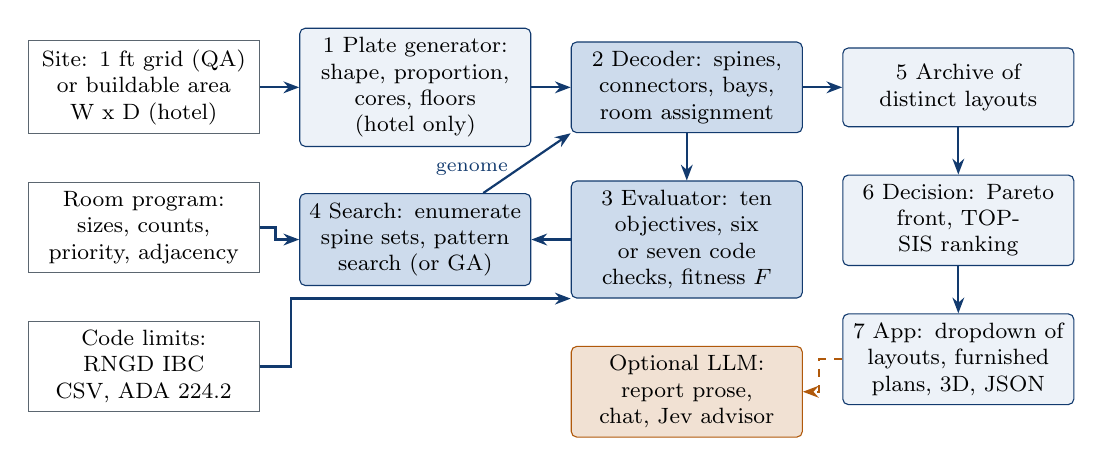
\begin{tikzpicture}[node distance=6mm and 5mm, every node/.style={font=\footnotesize},
 box/.style={draw=bpdeep, fill=bp!8, rounded corners=2pt, align=center, minimum height=10mm, text width=27mm},
 data/.style={draw=muted, fill=white, align=center, minimum height=9mm, text width=27mm},
 ai/.style={box, fill=warn!18, draw=warn}, loop/.style={box, fill=bp!22},
 arr/.style={-{Stealth[length=2mm]}, thick, bpdeep}]
\node[data] (site) {Site: 1 ft grid (QA) or buildable area W x D (hotel)};
\node[data, below=of site] (prog) {Room program: sizes, counts, priority, adjacency};
\node[data, below=of prog] (code) {Code limits: RNGD IBC CSV, ADA 224.2};
\node[box, right=of site] (plate) {1 Plate generator: shape, proportion, cores, floors (hotel only)};
\node[loop, right=of plate] (dec) {2 Decoder: spines, connectors, bays, room assignment};
\node[loop, below=of dec] (eval) {3 Evaluator: ten objectives, six or seven code checks, fitness $F$};
\node[loop, left=of eval] (search) {4 Search: enumerate spine sets, pattern search (or GA)};
\node[box, right=of dec] (arch) {5 Archive of distinct layouts};
\node[box, below=of arch] (dm) {6 Decision: Pareto front, TOPSIS ranking};
\node[box, below=of dm] (ui) {7 App: dropdown of layouts, furnished plans, 3D, JSON};
\node[ai, below=of eval] (llm) {Optional LLM: report prose, chat, Jev advisor};
\draw[arr] (site) -- (plate); \draw[arr] (plate) -- (dec); \draw[arr] (dec) -- (eval);
\draw[arr] (eval) -- (search); \draw[arr] (search) -- node[left, pos=0.4]{\scriptsize genome} (dec.south west);
\draw[arr] (prog.east) -- ++(2mm,0) |- (search.west); \draw[arr] (code.east) -- ++(4mm,0) |- (eval.south west);
\draw[arr] (dec) -- (arch); \draw[arr] (arch) -- (dm); \draw[arr] (dm) -- (ui);
\draw[arr, dashed, warn] (ui.west) -- ++(-3mm,0) |- (llm.east);
\end{tikzpicture}
\caption{Architecture of the layout optimizer. The darker boxes form the optimization loop and are deterministic.
The language model (orange) sits outside the loop: it only writes report prose, answers chat questions, or, if a
TypeSafe key is configured, advises on the final shortlist.}
\end{figure}
{\small\begin{longtable}{p{0.5cm}p{3.6cm}p{3.8cm}p{7.6cm}}\toprule
\textbf{\#} & \textbf{Component} & \textbf{File} & \textbf{What it does} \\ \midrule \endhead
1 & Plate generator & \texttt{optimize/typology.py} & Turns the hotel program into rooms with BaaP sizes; generates Bar, L, U, T, H and Courtyard plates inside the buildable area, with the elevator core and stairs placed by scheme (ends, centre, knuckle); one site grid per plate. \\
2 & Decoder & \texttt{optimize/planner.py} & Genome $\to$ corridor spines $\to$ orthogonal connectors $\to$ modular bays $\to$ rooms assigned to bays. Every output is a valid plan. \\
3 & Evaluator & \texttt{optimize/metrics.py} & Ten objectives in $[0,1]$, the code checks (exits, exit separation, travel, corridor width, dead end, ADA; stories for the hotel) and the fitness $F$. Limits come from RNGD's IBC CSV. \\
4 & Search & \texttt{optimize/search.py}, \texttt{explore.py} & Systematic enumeration of spine sets plus pattern search (default) or the memetic GA; for the hotel, all plates are screened in parallel processes and the best of each shape refined. \\
5 & Archive & \texttt{optimize/explore.py} & Keeps every distinct layout with its objectives and criteria. \\
6 & Decision & \texttt{optimize/decide.py} & Pareto front and TOPSIS ranking over twelve criteria; optional Jev advisor (TypeSafe) on the shortlist only. \\
7 & Views & \texttt{optimize/plan\_view.py}, \texttt{hotel\_opt\_ui.py}, \texttt{optimizer\_ui.py} & Dropdown of the top or all layouts, furnished interactive plans, 3D massing, comparison charts, JSON export. \\
-- & Reference loader & \texttt{optimize/baseline.py} & Rebuilds the reference designs from \texttt{QA/floorplan*.json} so they are scored by the same evaluator (their shared-wall lengths reproduce the values stored in the files). \\
-- & Report writer & \texttt{optimize/report.py} & One LLM call (\texttt{anthropic/claude-sonnet-5.5} through OpenRouter) writes the prose of the per-run PDF from the computed data and retrieved code passages; every number in its text is traced back to the data. \\
\bottomrule\end{longtable}}
Only the last row uses a language model. Steps 1 to 6 are plain Python on NumPy, SciPy and scikit-image arrays, so the
same inputs always give the same layouts and the same ranking.

\subsection{What was wrong, and how it was solved}
The problems below were seen in the reference results, in the first version of this app's optimizer (which followed the
same idea and added an LLM reviewer to the fitness) and in the team review of 10/08/2026.
{\small\begin{longtable}{p{3.3cm}p{3.7cm}p{4.9cm}p{3.6cm}}
\toprule
\textbf{Observed problem} & \textbf{Cause} & \textbf{What was changed} & \textbf{Evidence in this run} \\ \midrule \endhead
Guest rooms with no window; corridors loaded on one side only (review in the 10/08 meeting). & The corridor genome places segments anywhere; rooms are packed wherever they touch a corridor, so the distance to the facade is left to chance. & Decoder: corridor spines are chosen from lines scored for double-loaded window rooms (score $s(k)$); guest rooms may only take bays with a window (hard rule). & Windowless guest rooms over the three sites: 24 (A) $\to$ 0 (D). \\
Floor area left unused; rooms rotated or isolated. & Rooms are placed one by one as free rectangles, so leftovers between rooms cannot be used. & Modular bays of one room frontage $M$ along the whole corridor; rooms take whole bays, the last bay absorbs the remainder; unused bays are reported as flex space. & Unused share and corridor share per variant in Table~\ref{tab:optcompare}. \\
Not clear whether the requested keys can fit at all. & No bound was computed; the GA simply reports what it placed. & Area and window upper bounds, shown next to every result. & Table~\ref{tab:bounds}. \\
Crossover produces plans that do not make sense; slow convergence. & Half of one plan spliced onto half of another: the value of a corridor depends on the other corridors. & Search over a small structured space: enumerate spine sets, then first-improvement pattern search. The GA is kept as an option and now runs on the same decoder. & At the same budget D is within 0.010 fitness of the GA (C) with no crossover and no population: 192 against 197 rooms. Most of the gain over A comes from the decoder, not from the search. \\
With crossing corridors, facade strips stayed empty (seen on the square site fp2 in the first version of the new decoder: 39 rooms). & Bays were built corridor by corridor, so the windowless interior side of the first corridor took the strip that the next corridor's window rooms needed. & Two passes over all corridors: window bays first, windowless bays in what is left. & fp2: 60 rooms (D) and 62 (C), all guest rooms with a window. \\
Corridor stubs beyond the last room; dead ends over the 50 ft limit. & Spines were cut to the bays they could serve, not to the rooms actually placed. & After the assignment each spine is cut back to the doors and junctions it serves; the dead end is measured to the nearest exit door or through-route. & Longest dead end, D: 46 ft; A: 41 ft (same measure). \\
Runs take minutes; results change between runs. & 500 generations in the reference; an LLM reviewer inside the fitness in the earlier version of this app (about 10 minutes, cloud calls). & No LLM in the fitness; deterministic seeds; cached static scores in the assignment; plates evaluated in parallel processes. & Variant D: 59 s for the three sites; identical result on a repeat run: yes. \\
Egress and accessibility not part of the score. & The reference score rewards placed rooms and contiguity. & Ten objectives including exit travel, dead ends, ADA Table 224.2 count and dispersion, core access; limits read from RNGD's IBC CSV. & All variants pass the checks on these sites; the checks are now reported for every layout. \\
The shape, the core and the floor count are inputs. & The grid fixes the L-shaped plate and both cores. & Hotel Schematic: plates (six shapes), core schemes (three) and the floor count are generated and searched; a dropdown lists the top or all layouts. & 740 distinct layouts in 36 s (Section~\ref{sec:opthotel}). \\
\bottomrule
\end{longtable}}


\subsection{The mathematics}
\label{sec:optmath}
\paragraph{Problem.} A site is a stack of $L$ levels of 1 ft cells. On each level a set $\Omega$ of cells is
\emph{placeable}; cores (stairs, elevators) and structure are fixed in the QA sites and generated for the hotel. The program
is a list of room instances $i = 1..N$, each with a type $t(i)$, nominal frontage $f_i$ and depth $d_i$ (area
$\bar a_i = f_i d_i$), a priority $p_i$, a set of allowed levels and flags (needs a window, wants a corner, wants to be near a
core). A layout chooses a corridor $C \subset \Omega$ (the same on every level, so floors stack) and an axis-aligned rectangle
for some of the rooms, such that rectangles do not overlap each other or $C$, lie inside $\Omega$, and each room has a door on
$C$. The goal is to maximise the fitness $F$ below.

\paragraph{Decoder: from a short genome to a full layout.} The search never moves rooms directly. It works on a genome
$g \in [0,1]^{44+N}$ (ten candidate spines with four genes each: two trims, a shift, an on/off gene; four connector genes;
one order key per room) and the decoder builds the layout:
\begin{enumerate}
\item \textbf{Module.} The bay width is the weighted median guest-room frontage,
$M = \operatorname{median}_w\{f_t\}$ with weights equal to the room counts; $D$ is the median guest-room depth and $w$ the
corridor width.
\item \textbf{Candidate spines.} Every row and column $k$ that can hold a straight corridor band gets the score
\[ s(k) = \sum_{x \in \text{band}(k)} \big[\, g_a(x) + g_b(x) + 1.5\,n_a(x) + 1.5\,n_b(x) + 0.5\,r_a(x) + 0.5\,r_b(x) \,\big], \]
where, for the two sides $a$ and $b$ of the band at position $x$, $g=1$ if a room at least $0.92\,d_{\min}$ deep fits,
$n=1$ if in addition the facade is about one room depth away (a window room), and $r=1$ if it is within the deepest room's
depth. So a line that is double-loaded with window rooms on both sides scores $2 \times (1 + 1.5 + 0.5) = 6$ per foot, a
single-loaded line 3, and a line through deep space with no facade 2. The best non-overlapping lines (at least $d_{\min}+w$
apart) become the ten candidates.
\item \textbf{Connectors.} Active spines are trimmed to their last room and joined to each other and to every core with
orthogonal L-shaped paths (never diagonal); pieces that stay unconnected are dropped.
\item \textbf{Bays.} Each side of each straight corridor run of length $\ell$ is cut into
$n = \lfloor \ell / M \rfloor$ bays. The remainder $\rho = \ell - nM$ is absorbed by the last bay if $\rho < 0.4M$ and becomes
a narrow bay otherwise. A bay has a window if its back wall is on the facade. Bays are built in two passes over all
corridors, window bays first and windowless bays in what is left, so the interior side of one corridor never takes
the facade strip that another corridor's window rooms need.
\item \textbf{Assignment.} Rooms are taken in the order of $0.06\,p_i + g_i$ (priority, then the order key) and each takes
\[ k_i = \max\!\Big(\operatorname{round}\frac{\bar a_i}{M D},\ \Big\lceil \frac{0.85 f_i}{M} \Big\rceil\Big) \]
consecutive free bays on one allowed level, the run with the highest score
\begin{align*} \sigma ={}& W_{\text{ext}}\,[\text{window}] - W_{\text{nw}}\,[\text{no window}] + W_{\text{corner}}\,[\text{corner}]
+ W_{\text{core}}\Big(1 - \tfrac{\min(\delta,150)}{150}\Big) + W_{\text{adj}}\,A \\
&+ W_{\text{stack}}\,\tfrac{\min(S,2)}{2} + W_{\text{grp}}\,[\text{same type next door}] - 1.2\max(0, o - 1.2),
\end{align*}
with $\delta$ the corridor distance from the door to the nearest core, $A$ the adjacency credit, $S$ the number of floors
with the same room type in the same bay, and $o$ the ratio of the bay area to the room's nominal area. Two hard rules apply:
a guest room is only placed where every bay has a window, and only if the run gives at least 85\% of its nominal frontage
and depth.
\end{enumerate}
After the assignment, each spine is cut back to what it serves (the doors of placed rooms and its junctions with
other corridors and cores), which removes corridor stubs and shortens dead ends. The dead end $E$ is the longest
corridor distance from any corridor cell to the nearest exit door or through-route between two exits.

Every decoded layout is therefore valid by construction (straight corridors, rooms perpendicular to them, no overlaps, all
rooms on the corridor), and the search only has to decide \emph{which} corridors exist and \emph{in what order} rooms claim
bays.

\paragraph{Fitness.} Ten objectives $f_k \in [0,1]$ (1 is best) are combined with weights $w_k$:
\[ F = \frac{\sum_k w_k f_k}{\sum_k w_k} \; - \; \tfrac12 \max\!\big(0,\ \min(n_c, 2) - c\big), \]
where $n_c$ is the number of cores and $c$ the number the corridor reaches (an exit that is not connected costs half the
scale). With $\rho$ the corridor share of the plate, $T$ the longest exit travel and $E$ the longest dead end:
\begin{align*}
f_{\text{place}} &= \frac{\sum_{i\ \text{placed}} p_i \min(a_i, \bar a_i)}{\sum_{i} p_i \bar a_i}, &
f_{\text{day}} &= \frac{\#\{\text{rooms needing a window that have one}\}}{\#\{\text{rooms needing a window}\}}, \\
f_{\text{eff}} &= \operatorname{clip}\!\Big(1 - \frac{\rho}{0.30}\Big), &
f_{\text{egress}} &= 1 - \tfrac12 \min\!\Big(1, \frac{(T - 250)^+}{250}\Big) - \tfrac12 \min\!\Big(1, \frac{(E - 50)^+}{50}\Big), \\
f_{\text{ada}} &= \min\!\Big(1, \frac{n_{\text{ADA}}}{n_{224.2}}\Big)\cdot\min\!\Big(1, \frac{\text{floors with ADA}}{\text{target}}\Big), &
f_{\text{core}} &= \operatorname{mean}_i \Big(1 - \frac{\min(\delta_i, 120)}{120}\Big), \\
f_{\text{adj}} &= \frac{\sum_j \omega_j \max\big(0,\ 1 - (\Delta_j - m_j)^+/m_j\big)}{\sum_j \omega_j}, &
f_{\text{corner}} &= \frac{\#\{\text{corner rooms on a corner}\}}{\#\{\text{corner rooms}\}}, \\
f_{\text{bal}} &= \operatorname{clip}\!\Big(1 - \frac{\operatorname{sd}(K_\ell)}{\operatorname{mean}(K_\ell)}\Big), &
f_{\text{comp}} &= \operatorname{clip}\!\Big(\frac{2 S_{\text{shared}}}{0.6\, P_{\text{rooms}}}\Big).
\end{align*}
Here $a_i$ is the drawn area (credit is capped at the nominal area, so an oversized room is not worth more),
$\Delta_j$ the distance between the two rooms of adjacency $j$ with allowed distance $m_j$, $K_\ell$ the keys on guest floor
$\ell$, $S_{\text{shared}}$ the total length of walls shared by two rooms and $P_{\text{rooms}}$ the total room perimeter.
The limits 250 ft (exit travel) and 50 ft (dead end) are read from RNGD's IBC rule CSV. The weights are
placement 0.3, daylight 0.14, efficiency 0.1, egress 0.12, ada 0.08, core access 0.07, adjacency 0.07, corner 0.03, balance 0.05, compactness 0.04. There is no language model in $F$: it is arithmetic on the geometry.

\paragraph{Upper bounds (can the keys fit at all?).} Two bounds hold for any layout, whatever the algorithm.
A corridor of width $w$ serves at most two room depths, so at least $w/(2D+w)$ of the used floor is corridor:
\[ K \le K_{\text{area}} = \Big\lfloor \frac{L\,|\Omega|\,\big(1 - \tfrac{w}{2D+w}\big)}{\bar a} \Big\rfloor . \]
If every guest room needs a window, the rooms of one floor share the facade length $P_f$:
\[ K \le K_{\text{window}} = L \Big\lfloor \frac{P_f}{\bar f} \Big\rfloor . \]
For a generated hotel plate with corridor length $R$ and cores taking a frontage $c_f$, the bound per floor is
$\lfloor (2R - c_f)/M \rfloor$. The bounds are loose (they ignore corners and the public rooms), but a request above them
is impossible, and a result close to them is close to the best any search can do.

\paragraph{Search.} With $m$ candidate spines the decoder is driven by a subset of them, so the first stage enumerates
\[ 1 + \sum_{k=1}^{4} \binom{\min(m,7)}{k} \le 1 + 7 + 21 + 35 + 35 = 99 \]
spine sets (all spines, and every set of up to four of the seven best), with rooms in priority order. The second stage
starts from the three best distinct layouts and repeats: generate the neighbours (switch one spine on or off: 10 moves; trim
either end or shift an active spine: 4 moves each; new connector elbows; four room-order nudges), evaluate them in a seeded
random order, and accept the first one with $F' > F + 10^{-6}$. When all three starts are local optima, the rest of the budget is spent on iterated local search: the best
layout is ``kicked'' with two moves at once, improved again by the same pattern search, and kept only if it beats
the best so far. The total budget is $PG$ evaluations ($P$ = population, $G$ = generations, kept as the budget
controls), the same as the GA's. The genetic algorithm (variant C)
evaluates $P(G+1)$ layouts plus local-search steps, here about 804. Crossover is not used in the systematic search:
splicing the corridor genes of one plan with the room order of another seldom gives a better plan, because the value of a
corridor depends on which other corridors exist.

\paragraph{Plate generation (hotel).} For $K$ keys on $F$ guest floors the busiest level needs net area $A$; with slack
$\varsigma = 1.04$, core area $A_c$ and packing efficiency $\eta = 0.93$ the corridor length to provide is
\[ R = \frac{\varsigma A + A_c}{2 D \eta}. \]
Each shape with bounding box $a \times b$ and wing depth $W_d = 2D + w$ (58 ft) offers
$R_{\text{Bar}} = a$, $R_{\text{L}} = R_{\text{T}} = a + b - W_d$, $R_{\text{U}} = a + 2b - 2W_d$,
$R_{\text{H}} = a + 2b - 2W_d$ and $R_{\text{Courtyard}} = 2a + 2b - 4W_d$; the generator solves $R_{\text{shape}}(a, \beta a) \ge R$
for the smallest $a$ at aspect ratios $\beta \in \{0.6, 1\}$ and clips the result to the buildable area in both
orientations. The elevator count is $e = \max(2, \lceil K/75 \rceil)$, and the two stairs of the ``centre core'' scheme are
the pair of wing-end positions with the largest distance between them (exit separation, short dead ends).

\paragraph{Decision.} Each layout $j$ has a vector of twelve criteria $x_{j1..12}$ (keys, gross SF per key, facade per key,
height, corridor share, dead end, code checks passed and others). Layout $j$ is \emph{dominated} if another layout is at
least as good on every criterion and strictly better on one; the rest form the Pareto front. TOPSIS then ranks all layouts:
\[ r_{jq} = \frac{x_{jq}}{\sqrt{\sum_j x_{jq}^2}}, \quad v_{jq} = \frac{\lambda_q}{\sum_q \lambda_q}\, r_{jq}, \quad
d_j^{\pm} = \sqrt{\sum_q (v_{jq} - v_q^{\pm})^2}, \quad C_j = \frac{d_j^-}{d_j^+ + d_j^-} \in [0,1], \]
where $v_q^+$ is the best and $v_q^-$ the worst value of criterion $q$ over all layouts and $\lambda_q$ the weight from the
chosen preset (Balanced, Most keys, Lowest cost, Guest experience, Low-rise) or the sliders. The layout with the largest
$C_j$ is ranked first.


\subsection{Results on the three QA sites}\label{sec:optqa}
All variants use \texttt{QA/rooms\_hotel.json} (72 rooms on three levels) and are scored by the same evaluator. Variants
B, C and D were run with population 24 and 30 generations as the budget, seed 7, no LLM.
For A the search time is not stored in the files; its history holds 500 generations.
\begingroup\captionof{table}{Reference GA and the three later variants. ``No window'' counts guest rooms without a facade wall; ``Unused'' is the share of placeable area that is neither room nor corridor; ``Checks'' are the code checks passed.}\label{tab:optcompare}\endgroup
{\small\begin{longtable}{p{0.8cm}p{2.9cm}p{1.1cm}p{1.2cm}p{1.1cm}p{1.2cm}p{1.1cm}p{1.3cm}p{1.0cm}p{1.5cm}p{1.0cm}}
\toprule
\textbf{Site} & \textbf{Variant} & \textbf{Rooms} & \textbf{No window} & \textbf{Fitness} & \textbf{Corridor} & \textbf{Unused} & \textbf{Dead end ft} & \textbf{Checks} & \textbf{Evaluated} & \textbf{Time} \\ \midrule \endhead
fp1 & A Reference GA & 61/72 & 7 & 0.880 & 0.151 & 0.16 & 33 & 6/6 & 500 gen. & n/a \\
 & B GA, free-form & 53/72 & 3 & 0.880 & 0.100 & 0.29 & 55 & 5/6 & 804 & 119 s \\
 & C Updated GA & 72/72 & 0 & 0.954 & 0.101 & 0.09 & 27 & 6/6 & 804 & 24 s \\
 & D Systematic & 72/72 & 0 & 0.950 & 0.101 & 0.09 & 25 & 6/6 & 695 & 20 s \\ \midrule
fp2 & A Reference GA & 53/72 & 8 & 0.860 & 0.117 & 0.26 & 31 & 6/6 & 500 gen. & n/a \\
 & B GA, free-form & 60/72 & 8 & 0.893 & 0.111 & 0.19 & 36 & 6/6 & 804 & 102 s \\
 & C Updated GA & 62/72 & 0 & 0.908 & 0.146 & 0.06 & 43 & 6/6 & 804 & 22 s \\
 & D Systematic & 60/72 & 0 & 0.904 & 0.145 & 0.09 & 46 & 6/6 & 637 & 17 s \\ \midrule
fp3 & A Reference GA & 57/72 & 9 & 0.851 & 0.157 & 0.18 & 41 & 6/6 & 500 gen. & n/a \\
 & B GA, free-form & 61/72 & 3 & 0.894 & 0.120 & 0.18 & 33 & 6/6 & 804 & 115 s \\
 & C Updated GA & 63/72 & 0 & 0.921 & 0.122 & 0.11 & 35 & 6/6 & 804 & 26 s \\
 & D Systematic & 60/72 & 0 & 0.911 & 0.119 & 0.09 & 29 & 6/6 & 683 & 21 s \\
\bottomrule
\end{longtable}}
\begingroup\captionof{table}{Upper bounds on the number of keys (Section~\ref{sec:optmath}) against what was asked and placed.}\label{tab:bounds}\endgroup
{\small\begin{longtable}{p{0.8cm}p{1.6cm}p{1.3cm}p{1.5cm}p{1.4cm}p{1.6cm}p{1.0cm}p{1.2cm}p{1.0cm}p{0.9cm}p{0.9cm}}
\toprule
\textbf{Site} & \textbf{Placeable SF / level} & \textbf{Program SF} & \textbf{Program / placeable} & \textbf{Facade ft / level} & \textbf{Mean key frontage ft} & \textbf{$K_{\text{area}}$} & \textbf{$K_{\text{window}}$} & \textbf{Keys asked} & \textbf{Keys A} & \textbf{Keys D} \\ \midrule \endhead
fp1 & 9,640 & 23,310 & 0.81 & 489 & 12.9 & 80 & 111 & 69 & 58 & 69 \\
fp2 & 9,446 & 23,310 & 0.82 & 410 & 12.9 & 78 & 93 & 69 & 50 & 57 \\
fp3 & 9,412 & 23,310 & 0.83 & 519 & 12.9 & 78 & 120 & 69 & 54 & 57 \\
\bottomrule
\end{longtable}}
\begin{figure}[H]\centering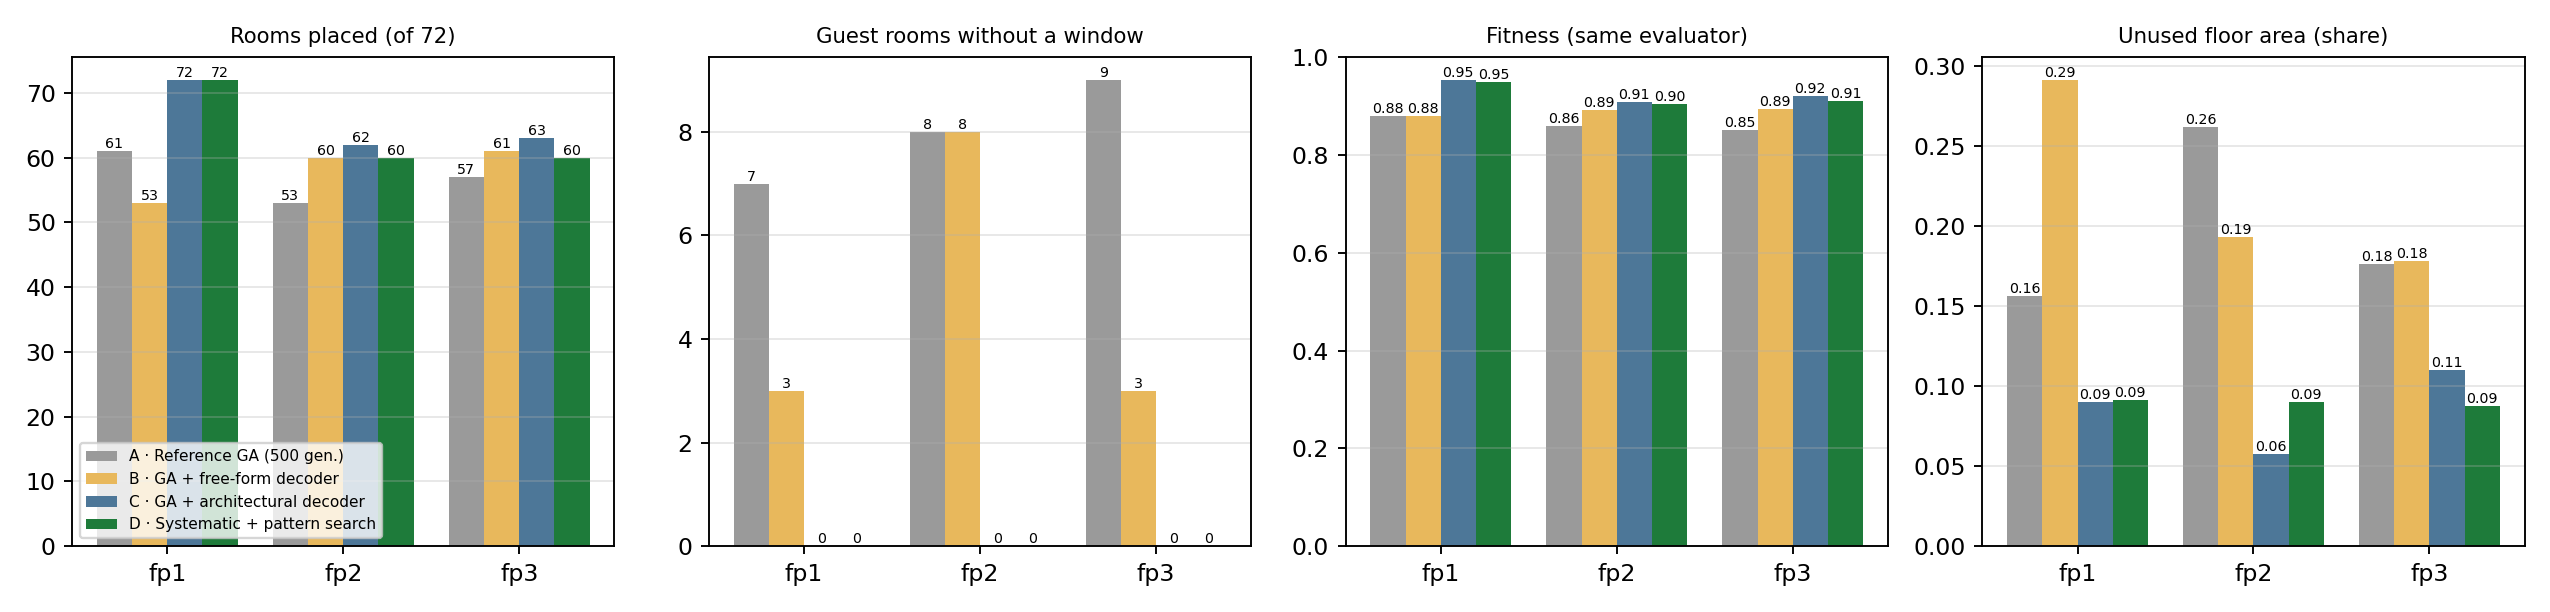
\includegraphics[width=\linewidth,keepaspectratio,height=0.30\textheight]{optimizer/compare_bars.png}\caption{The four variants on the three sites (same program, same evaluator).}\end{figure}
\begin{figure}[H]\centering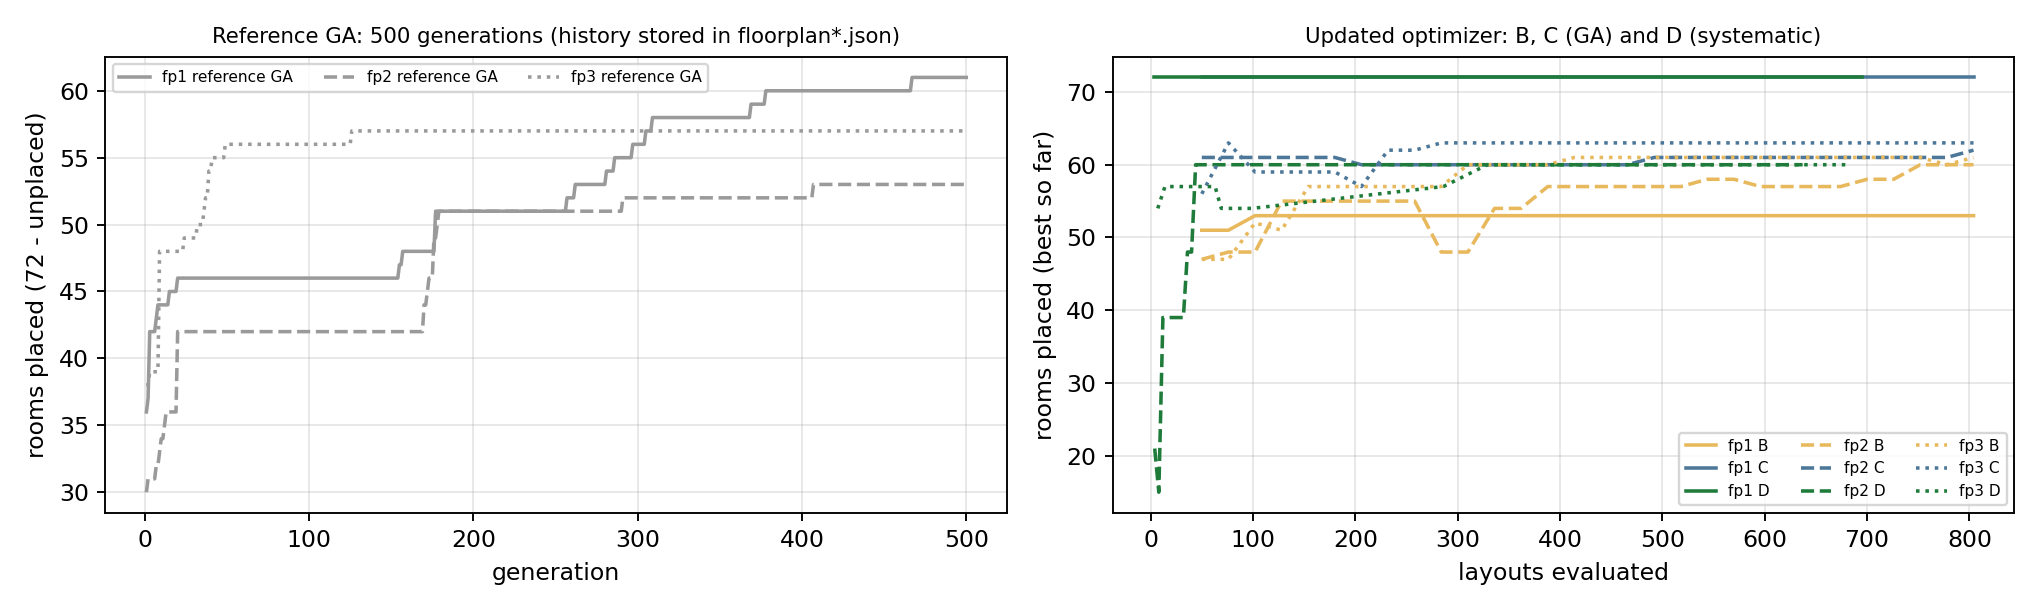
\includegraphics[width=\linewidth,keepaspectratio,height=0.30\textheight]{optimizer/convergence.png}\caption{Left: rooms placed by the reference GA over its generations (from the history in the delivered files). Right: best rooms placed against layouts evaluated for the later variants.}\end{figure}
\begin{figure}[H]\centering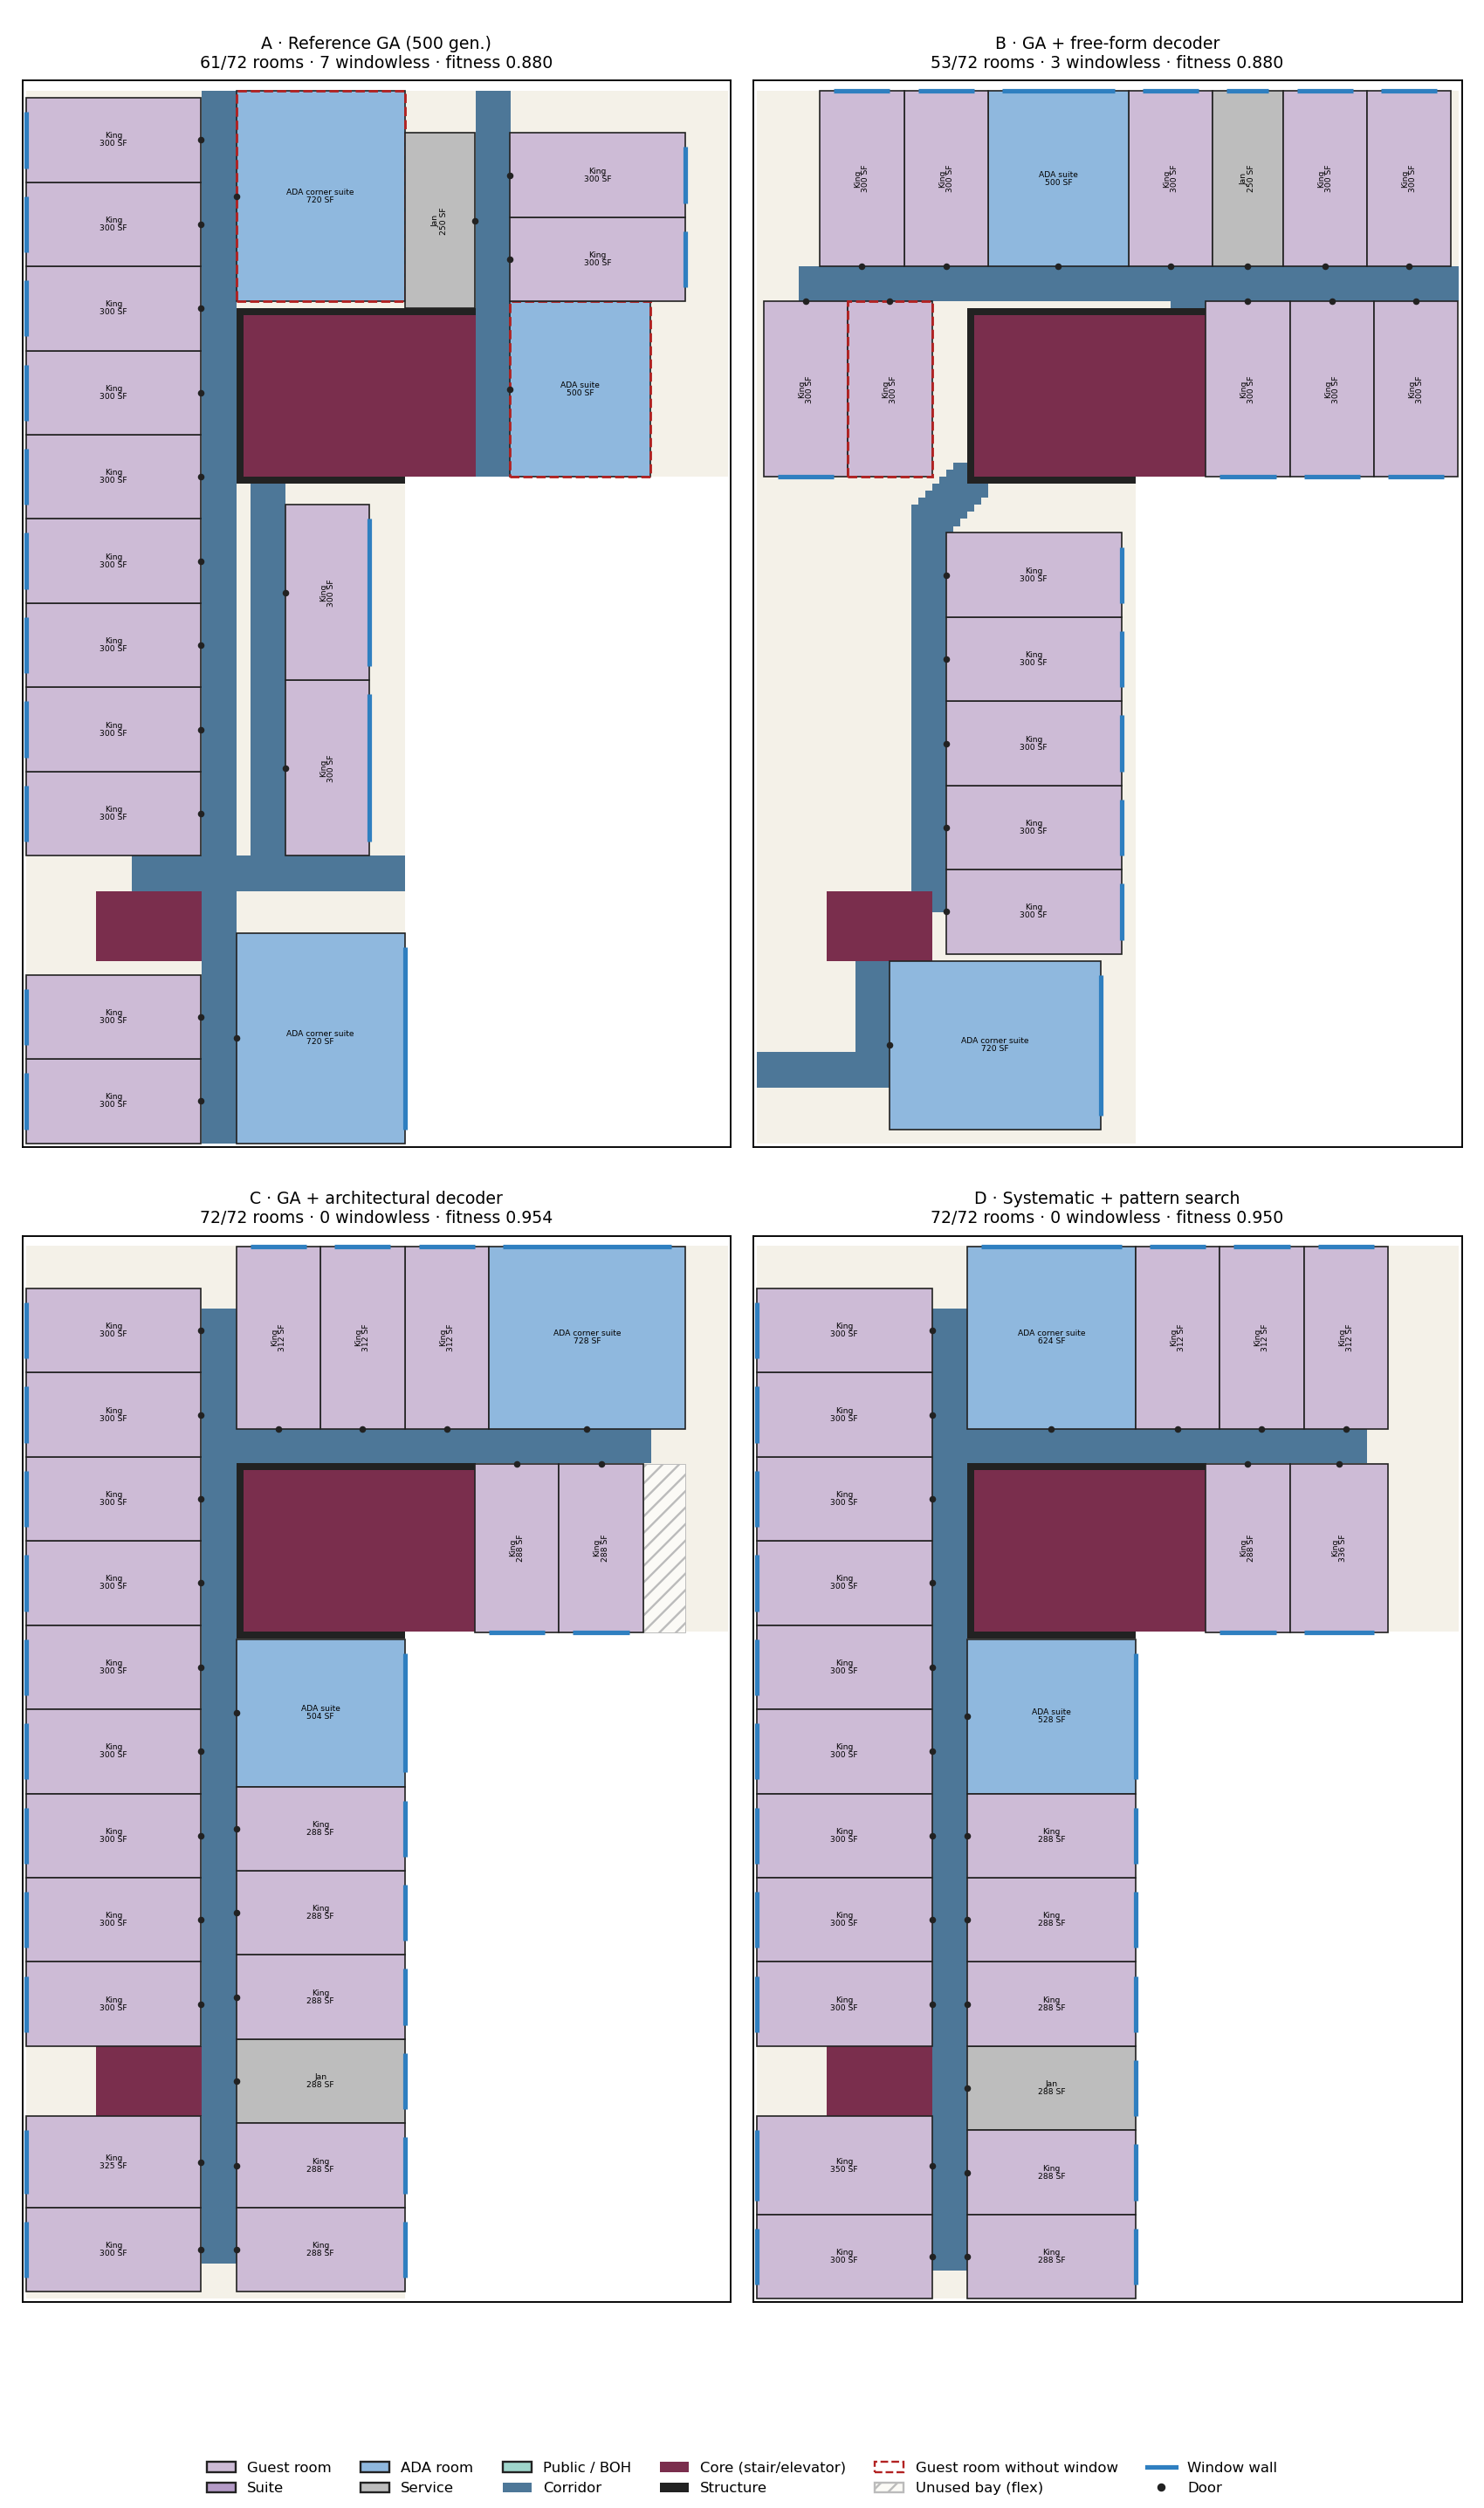
\includegraphics[width=\linewidth,keepaspectratio,height=0.80\textheight]{optimizer/compare_fp1.png}\caption{Site fp1, Level 2, same program and same evaluator. Blue lines are window walls; a red dashed outline marks a guest room with no window; hatched bays are unused.}\end{figure}
\begin{figure}[H]\centering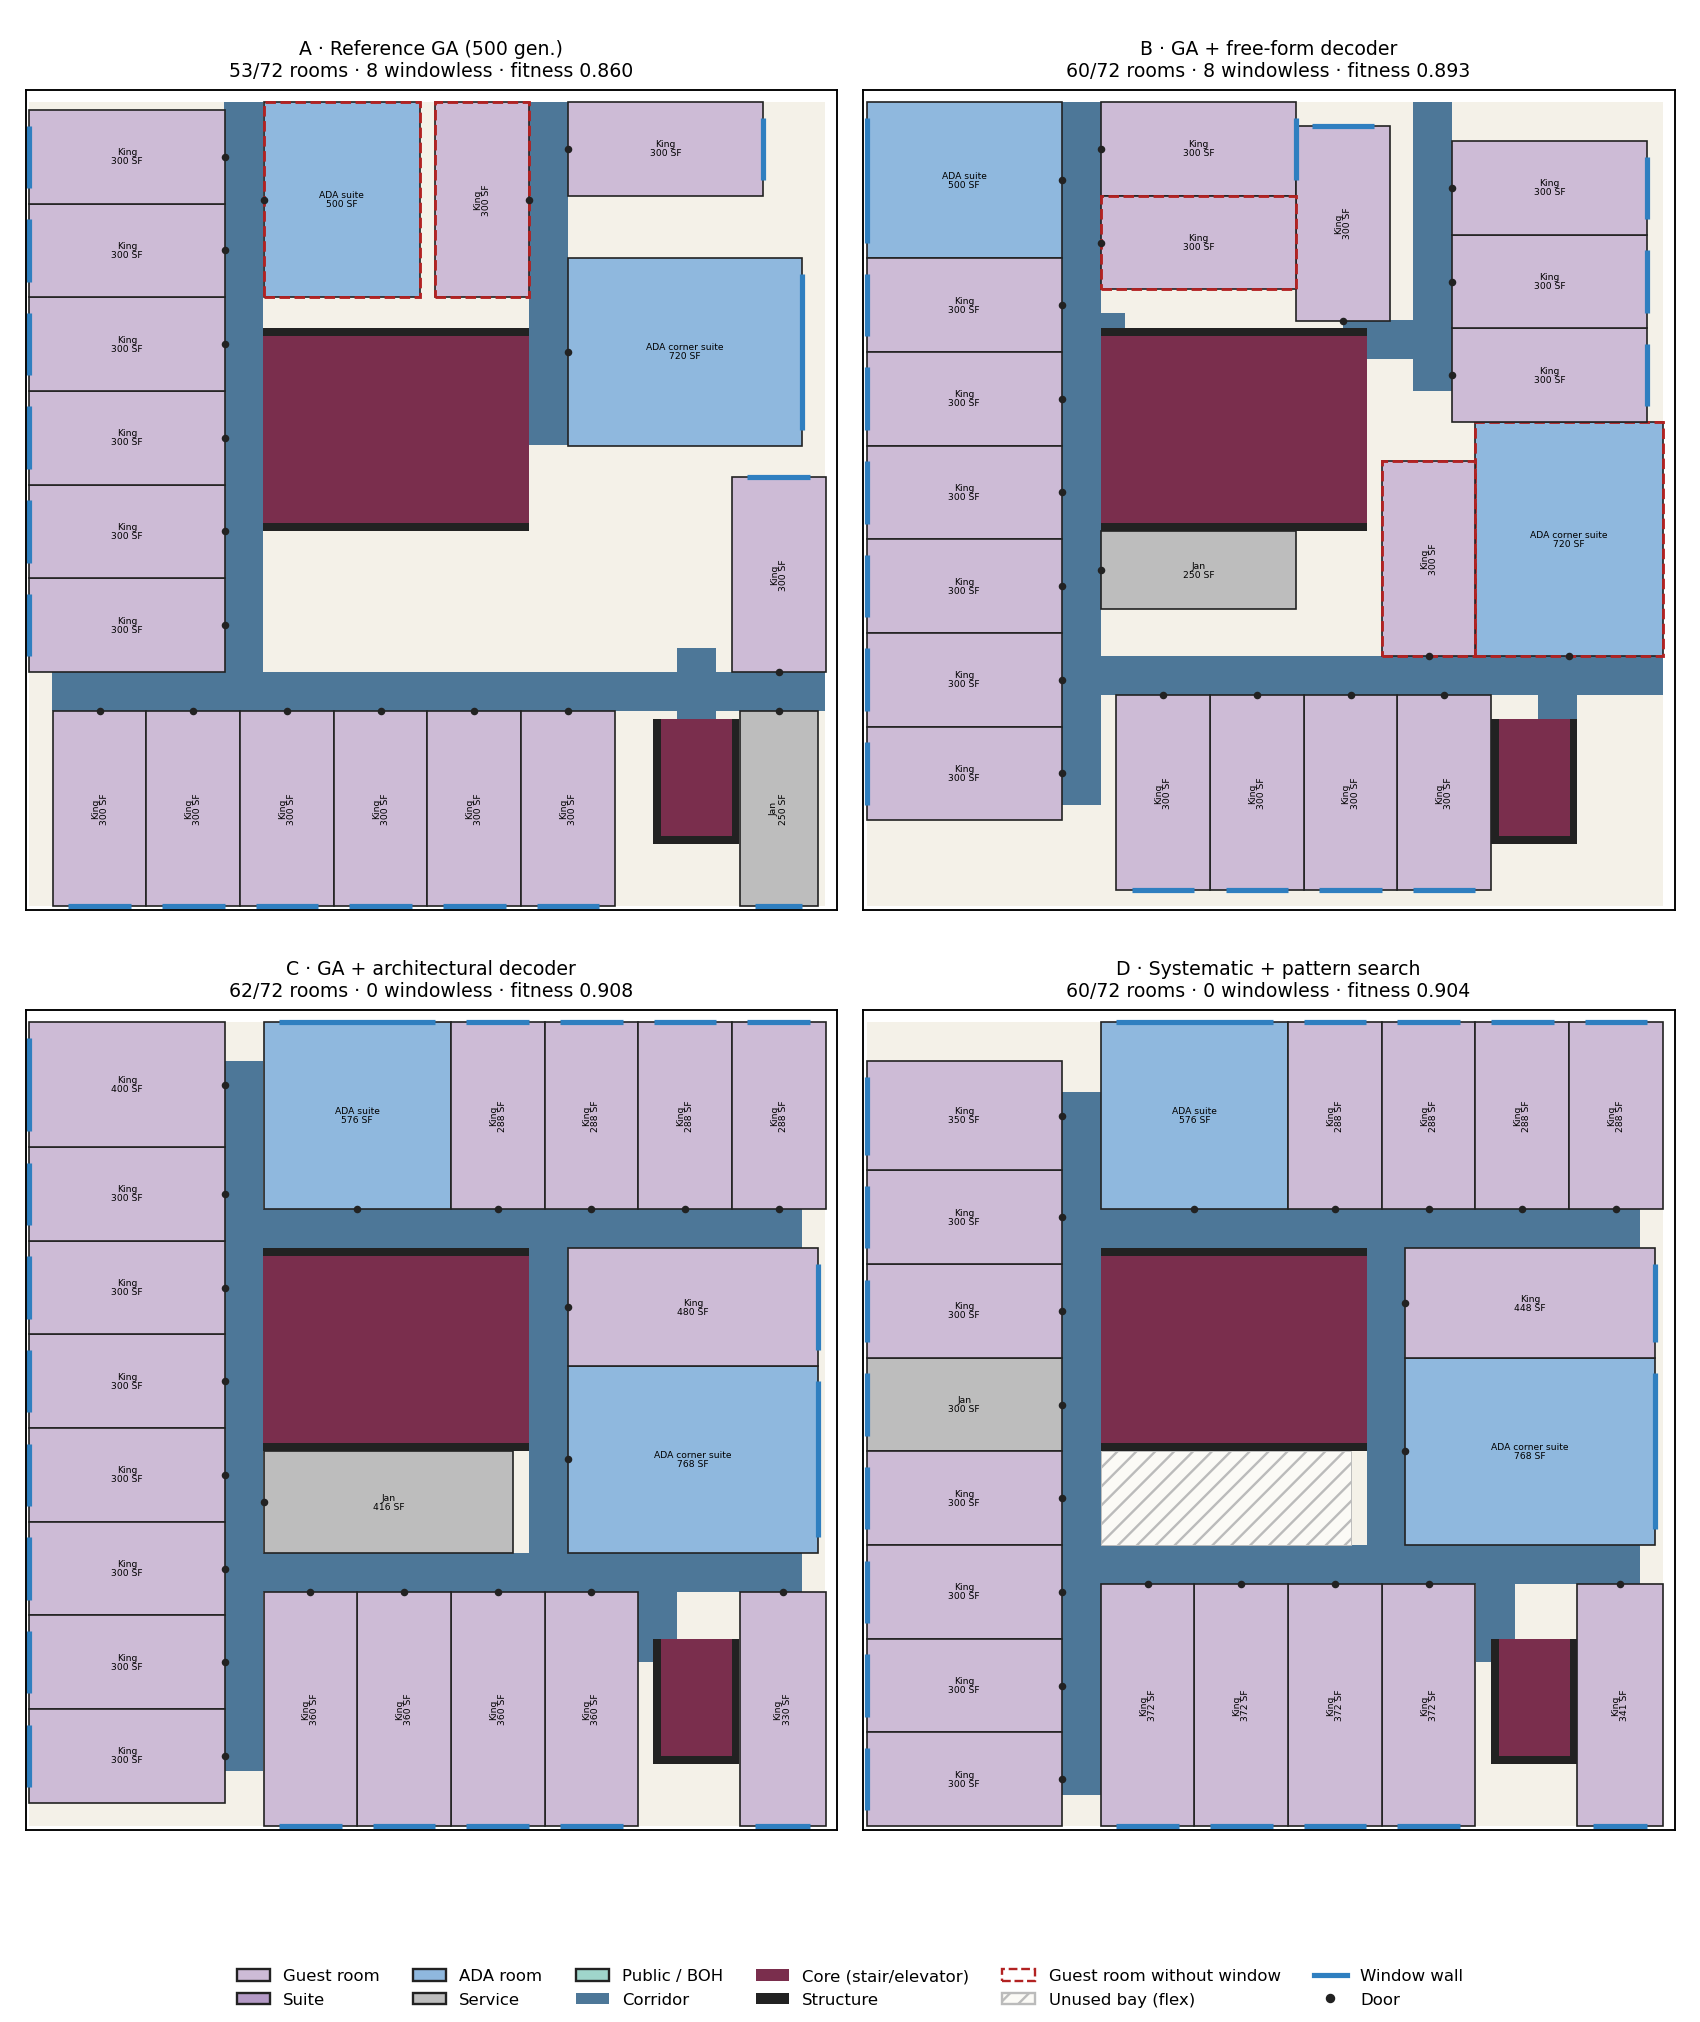
\includegraphics[width=\linewidth,keepaspectratio,height=0.80\textheight]{optimizer/compare_fp2.png}\caption{Site fp2, Level 2, same program and same evaluator. Blue lines are window walls; a red dashed outline marks a guest room with no window; hatched bays are unused.}\end{figure}
\begin{figure}[H]\centering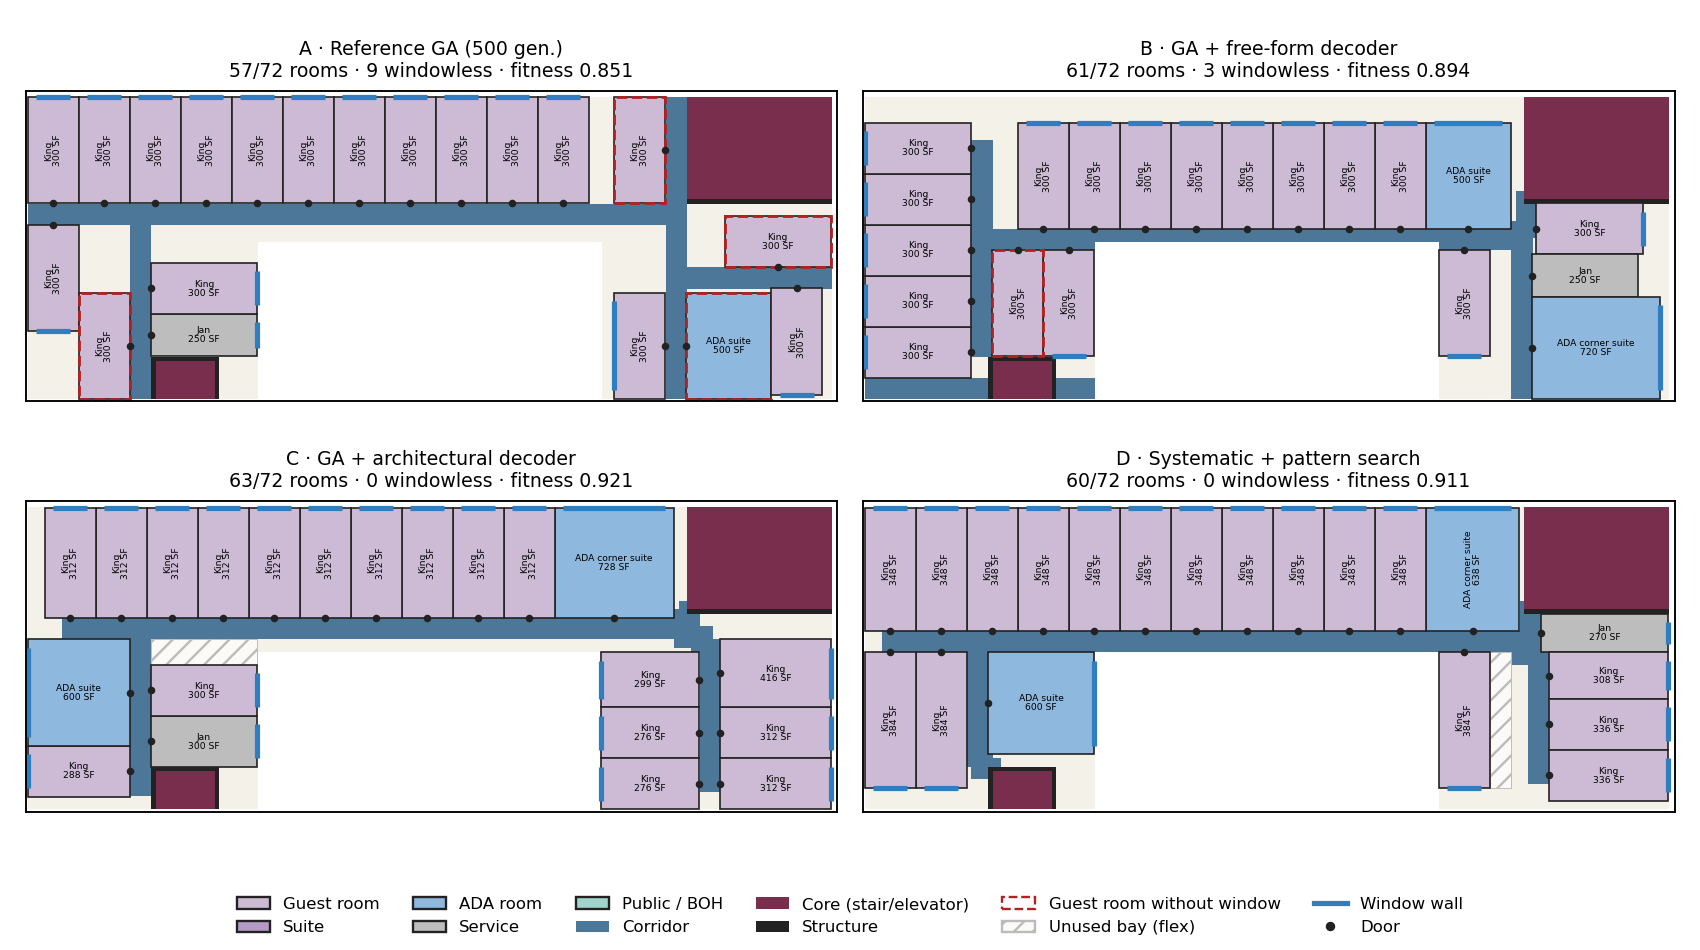
\includegraphics[width=\linewidth,keepaspectratio,height=0.80\textheight]{optimizer/compare_fp3.png}\caption{Site fp3, Level 2, same program and same evaluator. Blue lines are window walls; a red dashed outline marks a guest room with no window; hatched bays are unused.}\end{figure}

\subsection{Results in Hotel Schematic (generative shape, core and floors)}\label{sec:opthotel}
Input: the Project Renegade Living + Lodging program (117 keys) and a buildable area of
170 x 265 ft. The search screened 158 plate and floor-count variants,
evaluated 1,140 layouts and kept 740 distinct ones in 36 s on eight
processes, with no LLM calls; a second run returned the same list: yes.
212 layouts are on the Pareto front. Pattern search improved the screened plates as follows:
Courtyard 156x156 $\cdot$ center core (5 fl.) 0.870 $\to$ 0.870; L 202x121 $\cdot$ ends core (5 fl.) 0.863 $\to$ 0.881; Bar 265x58 $\cdot$ center core (5 fl.) 0.863 $\to$ 0.863; T 202x121 $\cdot$ center core (5 fl.) 0.856 $\to$ 0.865.
\begingroup\captionof{table}{Top ten layouts under the Balanced decision weights.}\endgroup
{\small\begin{longtable}{p{0.4cm}p{4.2cm}p{1.0cm}p{1.2cm}p{0.9cm}p{0.8cm}p{1.0cm}p{1.1cm}p{0.9cm}p{0.9cm}p{1.0cm}p{0.8cm}}
\toprule
\textbf{\#} & \textbf{Layout} & \textbf{Guest floors} & \textbf{TOPSIS $C_j$} & \textbf{Pareto} & \textbf{Keys} & \textbf{Fitness} & \textbf{Corridor} & \textbf{SF / key} & \textbf{Height ft} & \textbf{Dead end ft} & \textbf{Code} \\ \midrule \endhead
1 & Bar 265x58 $\cdot$ center core & 4 & 0.917 & yes & 117 & 0.859 & 0.112 & 657 & 59 & 24 & 1.00 \\
2 & L 220x132 $\cdot$ knuckle core & 4 & 0.906 & yes & 117 & 0.849 & 0.120 & 729 & 59 & 26 & 1.00 \\
3 & L 170x176 $\cdot$ knuckle core & 4 & 0.905 & yes & 117 & 0.835 & 0.120 & 714 & 59 & 24 & 1.00 \\
4 & Bar 265x58 $\cdot$ ends core & 4 & 0.904 & yes & 117 & 0.845 & 0.113 & 657 & 59 & 30 & 1.00 \\
5 & Bar 265x58 $\cdot$ ends core & 4 & 0.903 & yes & 117 & 0.843 & 0.113 & 657 & 59 & 30 & 1.00 \\
6 & Bar 265x58 $\cdot$ ends core & 4 & 0.903 & yes & 117 & 0.842 & 0.113 & 657 & 59 & 31 & 1.00 \\
7 & Courtyard 156x156 $\cdot$ ends core & 4 & 0.902 & yes & 117 & 0.845 & 0.111 & 972 & 59 & 28 & 1.00 \\
8 & T 170x176 $\cdot$ knuckle core & 4 & 0.899 & no & 114 & 0.840 & 0.122 & 733 & 59 & 24 & 1.00 \\
9 & T 170x176 $\cdot$ knuckle core & 4 & 0.899 & no & 114 & 0.840 & 0.122 & 733 & 59 & 24 & 1.00 \\
10 & Bar 265x58 $\cdot$ center core & 5 & 0.897 & yes & 117 & 0.863 & 0.112 & 788 & 70 & 24 & 0.86 \\
\bottomrule
\end{longtable}}
\begingroup\captionof{table}{Best layout of each shape (Balanced weights).}\endgroup
{\small\begin{longtable}{p{1.7cm}p{4.6cm}p{1.1cm}p{1.2cm}p{0.9cm}p{1.1cm}p{1.4cm}p{1.2cm}p{0.9cm}}
\toprule
\textbf{Shape} & \textbf{Best layout of that shape} & \textbf{Guest floors} & \textbf{Overall rank} & \textbf{Keys} & \textbf{SF / key} & \textbf{Facade ft / key} & \textbf{Dead end ft} & \textbf{Code} \\ \midrule \endhead
Bar & Bar 265x58 $\cdot$ center core & 4 & 1 & 117 & 657 & 27.6 & 24 & 1.00 \\
L & L 220x132 $\cdot$ knuckle core & 4 & 2 & 117 & 729 & 30.1 & 26 & 1.00 \\
Courtyard & Courtyard 156x156 $\cdot$ ends core & 4 & 7 & 117 & 972 & 33.5 & 28 & 1.00 \\
T & T 170x176 $\cdot$ knuckle core & 4 & 8 & 114 & 733 & 30.4 & 24 & 1.00 \\
U & U 187x112 $\cdot$ center core & 4 & 34 & 111 & 771 & 31.8 & 29 & 1.00 \\
H & H 156x136 $\cdot$ knuckle core & 4 & 206 & 106 & 854 & 34.9 & 59 & 0.86 \\
\bottomrule
\end{longtable}}
\begingroup\captionof{table}{The first-ranked layout changes with the decision priority: the trade-off is the user's, the search only supplies the options.}\endgroup
{\small\begin{longtable}{p{2.8cm}p{5.2cm}p{1.3cm}p{1.0cm}p{1.2cm}p{1.3cm}p{1.0cm}}
\toprule
\textbf{Decision priority} & \textbf{Layout ranked first} & \textbf{Guest floors} & \textbf{Keys} & \textbf{SF / key} & \textbf{Height ft} & \textbf{Code} \\ \midrule \endhead
Balanced & Bar 265x58 $\cdot$ center core & 4 & 117 & 657 & 59 & 1.00 \\
Most keys & Courtyard 156x156 $\cdot$ center core & 4 & 117 & 972 & 59 & 1.00 \\
Lowest cost & Bar 265x58 $\cdot$ center core & 4 & 117 & 657 & 59 & 1.00 \\
Guest experience & Bar 265x58 $\cdot$ center core & 4 & 117 & 657 & 59 & 1.00 \\
Low-rise & Bar 265x58 $\cdot$ center core & 4 & 117 & 657 & 59 & 1.00 \\
\bottomrule
\end{longtable}}
\textbf{First-ranked layout: Bar 265x58 $\cdot$ center core, 4 guest floors.} Footprint 265 x 58 ft
(15,370 SF), 2 elevators, bay module 13 ft. It places
117 of 117 keys and 142 of 150 program rooms; the
frontage bound is 34 keys per typical floor. Corridor share 0.112, longest exit
travel 64 ft, dead end 24 ft, fitness 0.859. Not placed: White Box Retail x1, IT x1, Jan x2, Gym x1, MEP Service x1, Loading x1, Luggage x1.
{\small\begin{longtable}{p{1.9cm}p{4.6cm}p{4.6cm}p{2.4cm}p{1.3cm}}
\toprule
\textbf{Rule} & \textbf{Check} & \textbf{Required} & \textbf{Provided} & \textbf{Status} \\ \midrule \endhead
IBC-R1-015 & Exits per story (cores reached) & $\ge$ 2 & 3 & \textcolor{pass}{\textbf{PASS}} \\
IBC-R1-018 & Exit separation (core to core) & $\ge$ 1/3 diagonal = 90 ft & 202 ft & \textcolor{pass}{\textbf{PASS}} \\
IBC-R1-023 & Exit access travel & $\le$ 250 ft & 63 ft & \textcolor{pass}{\textbf{PASS}} \\
IBC-R1-025 & Corridor width & $\ge$ 44 in & 72 in & \textcolor{pass}{\textbf{PASS}} \\
IBC-R1-027 & Dead-end corridor & $\le$ 50 ft & 24 ft & \textcolor{pass}{\textbf{PASS}} \\
ADA-224.2 & ADA mobility rooms & $\ge$ 7 for 117 keys & 7 & \textcolor{pass}{\textbf{PASS}} \\
IBC-R1-007 & Stories above grade & $\le$ 5 (Type IIA, sprinklered R-1) & 5 & \textcolor{pass}{\textbf{PASS}} \\
\bottomrule
\end{longtable}}
\begin{figure}[H]\centering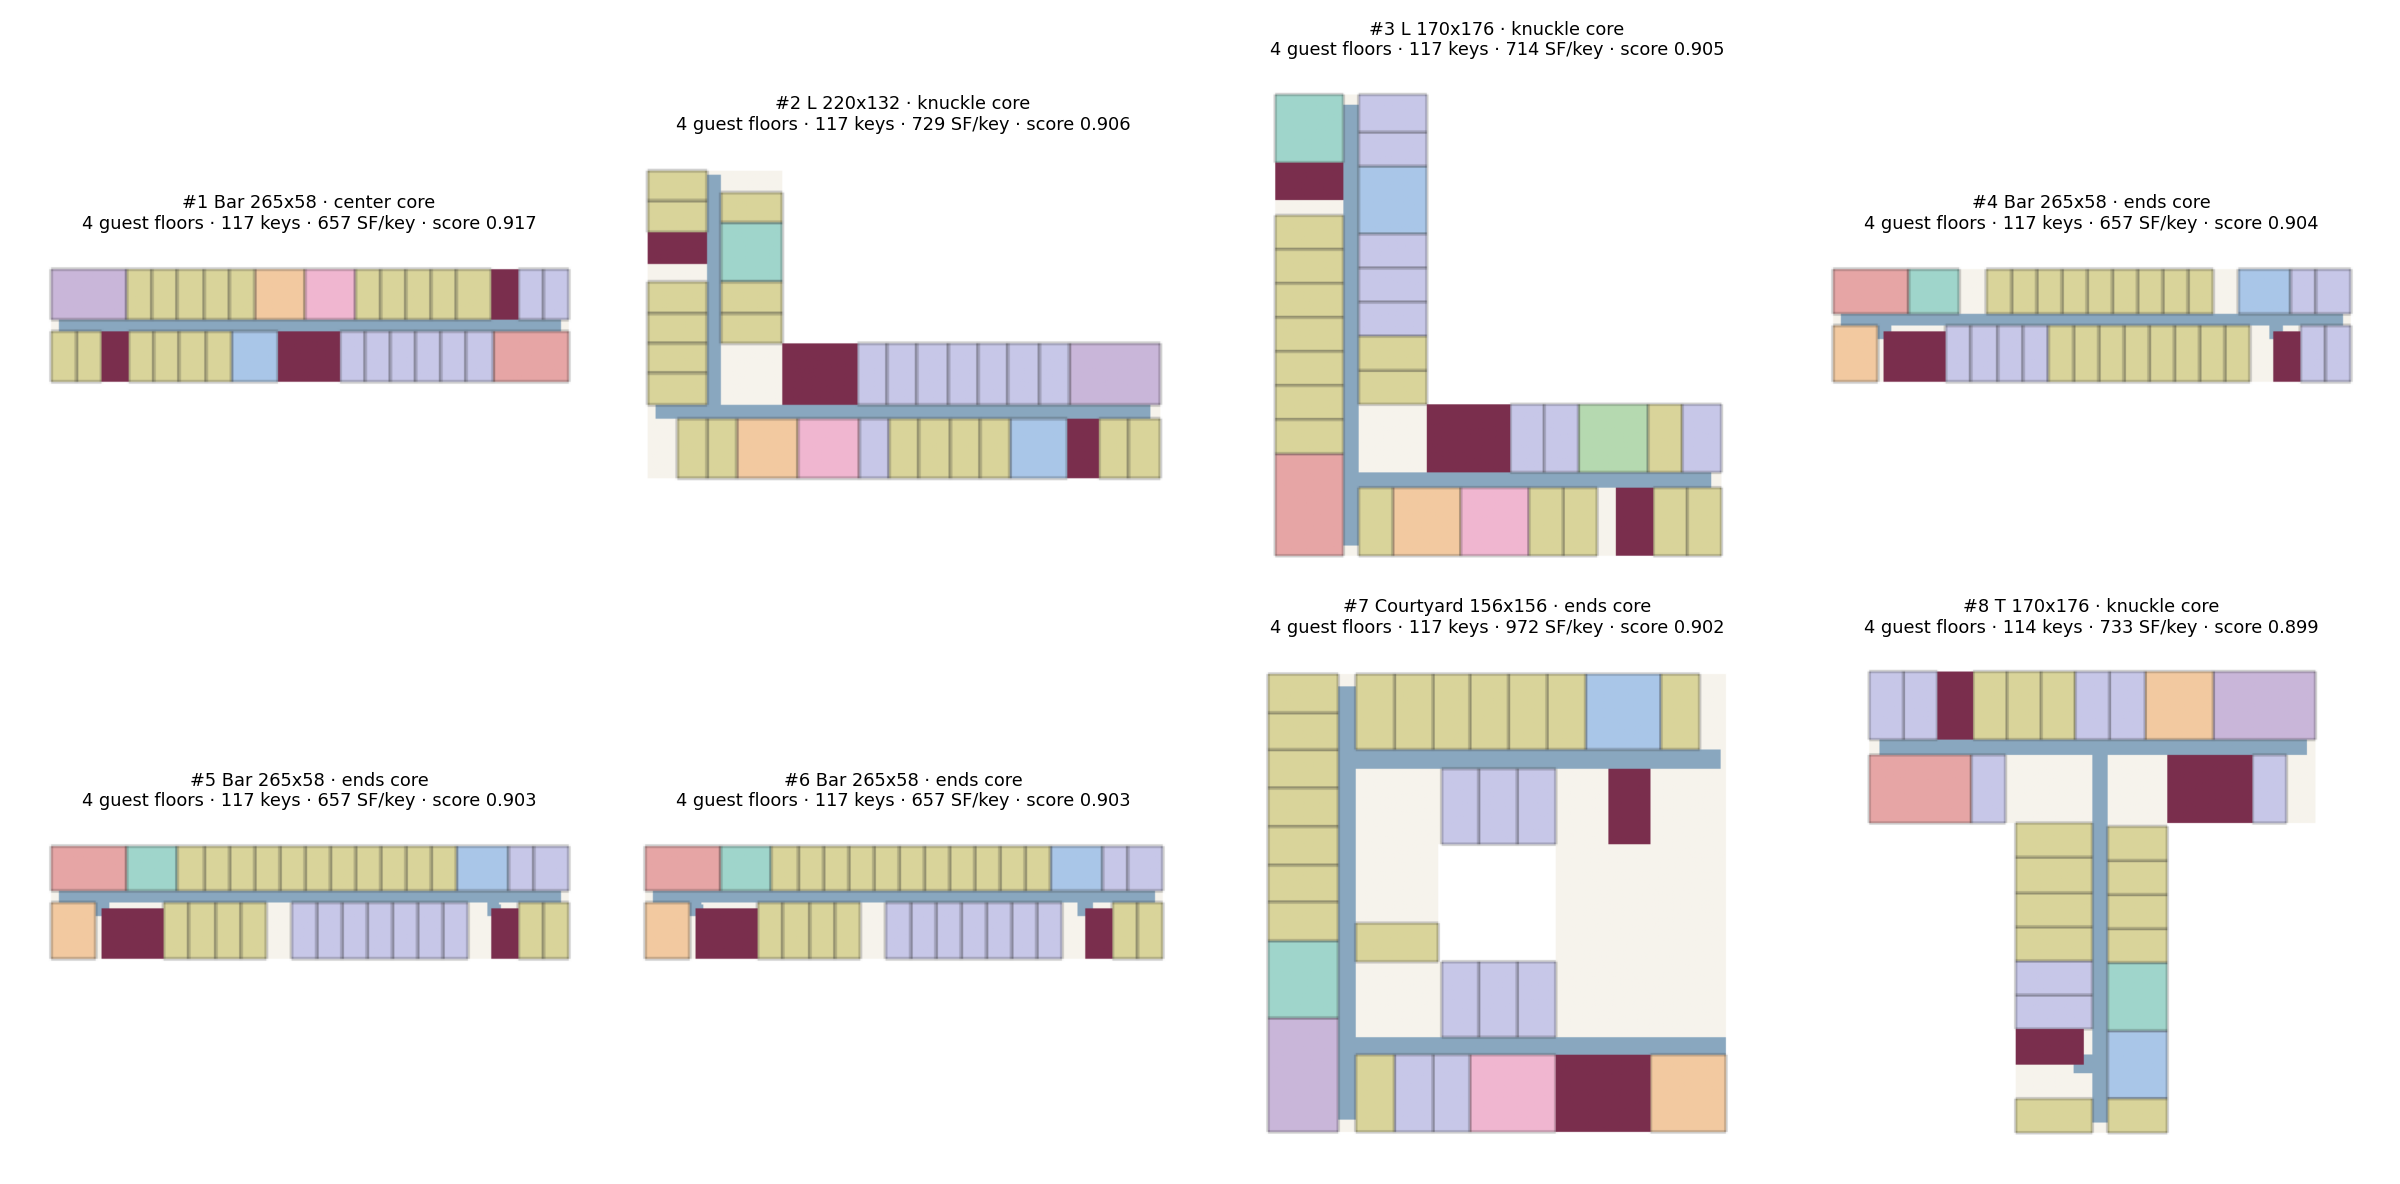
\includegraphics[width=\linewidth,keepaspectratio,height=0.45\textheight]{optimizer/hotel_gallery.png}\caption{The eight first-ranked layouts (typical guest floor). Dark red: core and stairs; blue: corridor.}\end{figure}
\begin{figure}[H]\centering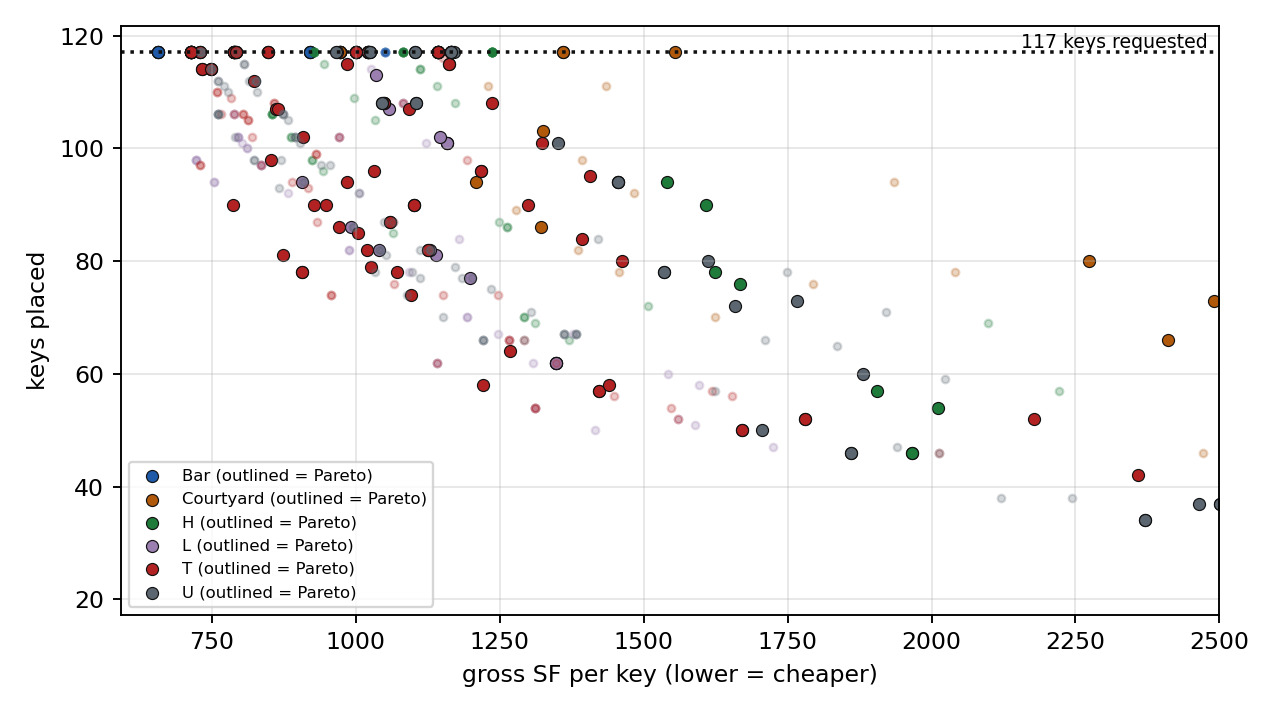
\includegraphics[width=\linewidth,keepaspectratio,height=0.34\textheight]{optimizer/hotel_pareto.png}\caption{Every layout found: keys placed against gross area per key. Outlined points are on the Pareto front.}\end{figure}
\begin{figure}[H]\centering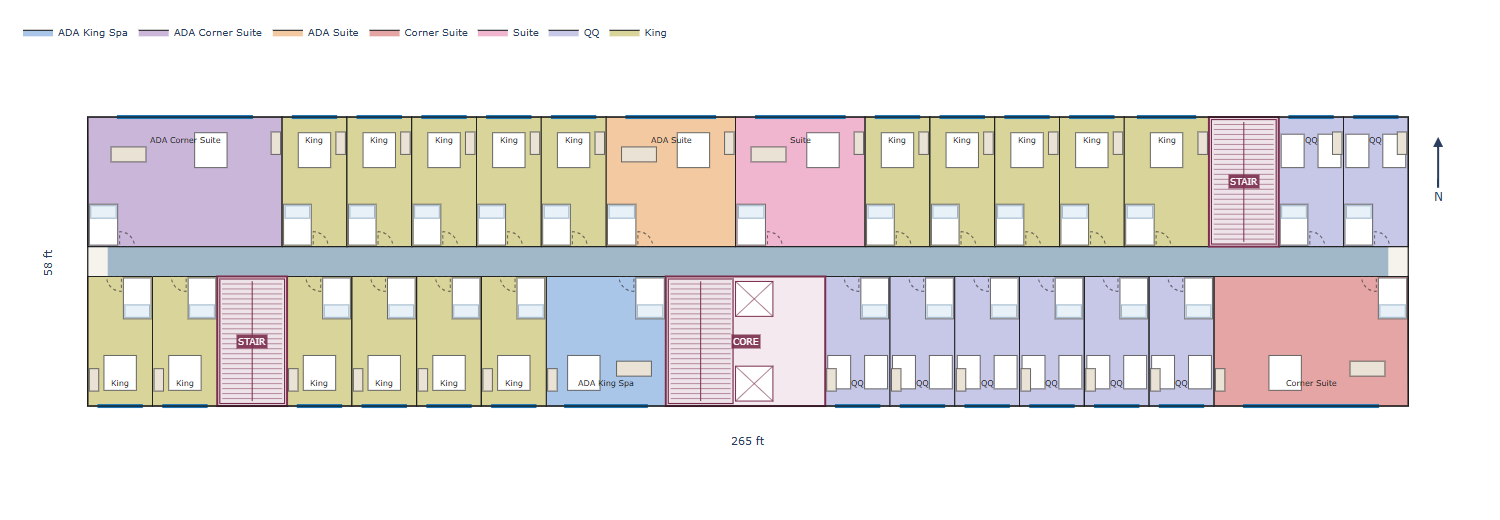
\includegraphics[width=\linewidth,keepaspectratio,height=0.40\textheight]{optimizer/hotel_best_L2.png}\caption{First-ranked layout, Level 2, as drawn in the app: furnished rooms, door swings, windows (blue), stairs and elevators.}\end{figure}
\begin{figure}[H]\centering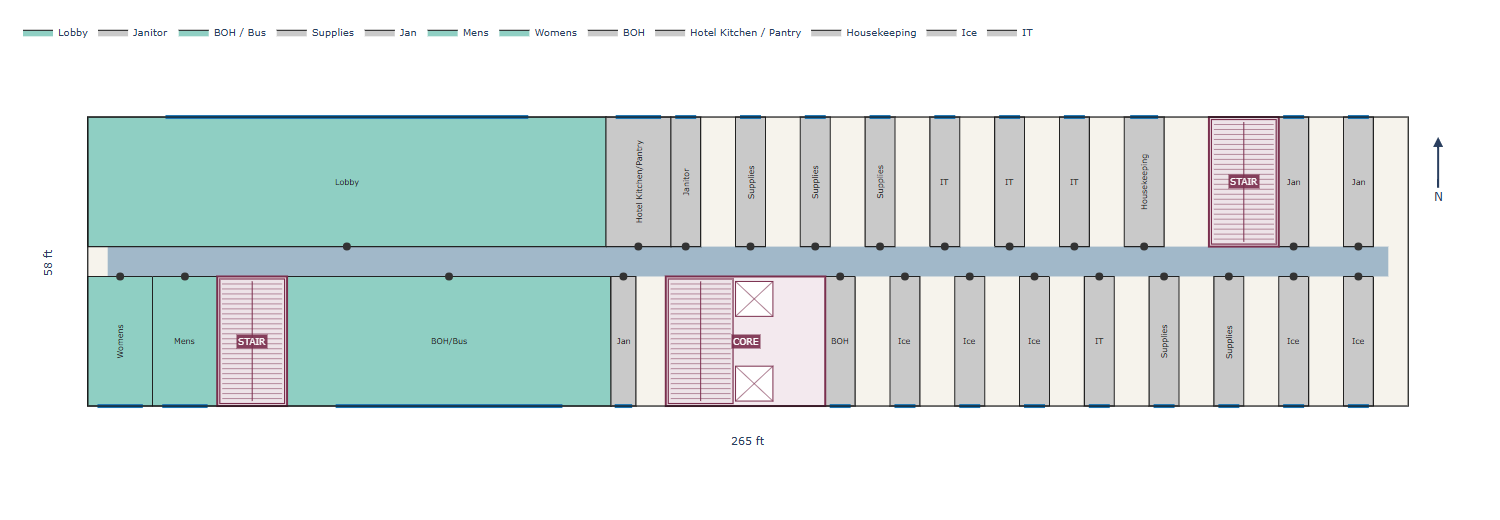
\includegraphics[width=\linewidth,keepaspectratio,height=0.40\textheight]{optimizer/hotel_best_L1.png}\caption{First-ranked layout, Level 1 (public and back-of-house rooms).}\end{figure}
\begin{figure}[H]\centering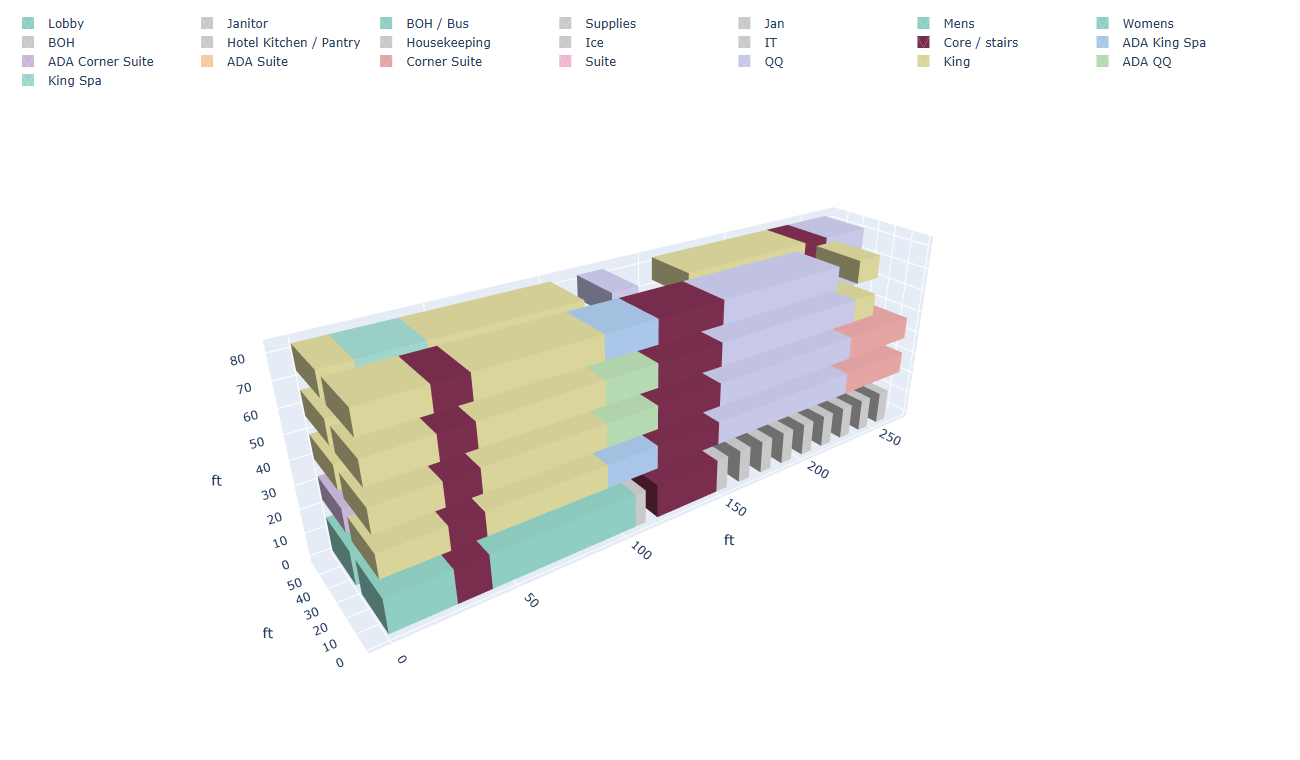
\includegraphics[width=\linewidth,keepaspectratio,height=0.38\textheight]{optimizer/hotel_best_3d.png}\caption{First-ranked layout, stacked massing with the floors pulled apart.}\end{figure}

\subsection{App screenshots}
\begin{figure}[H]\centering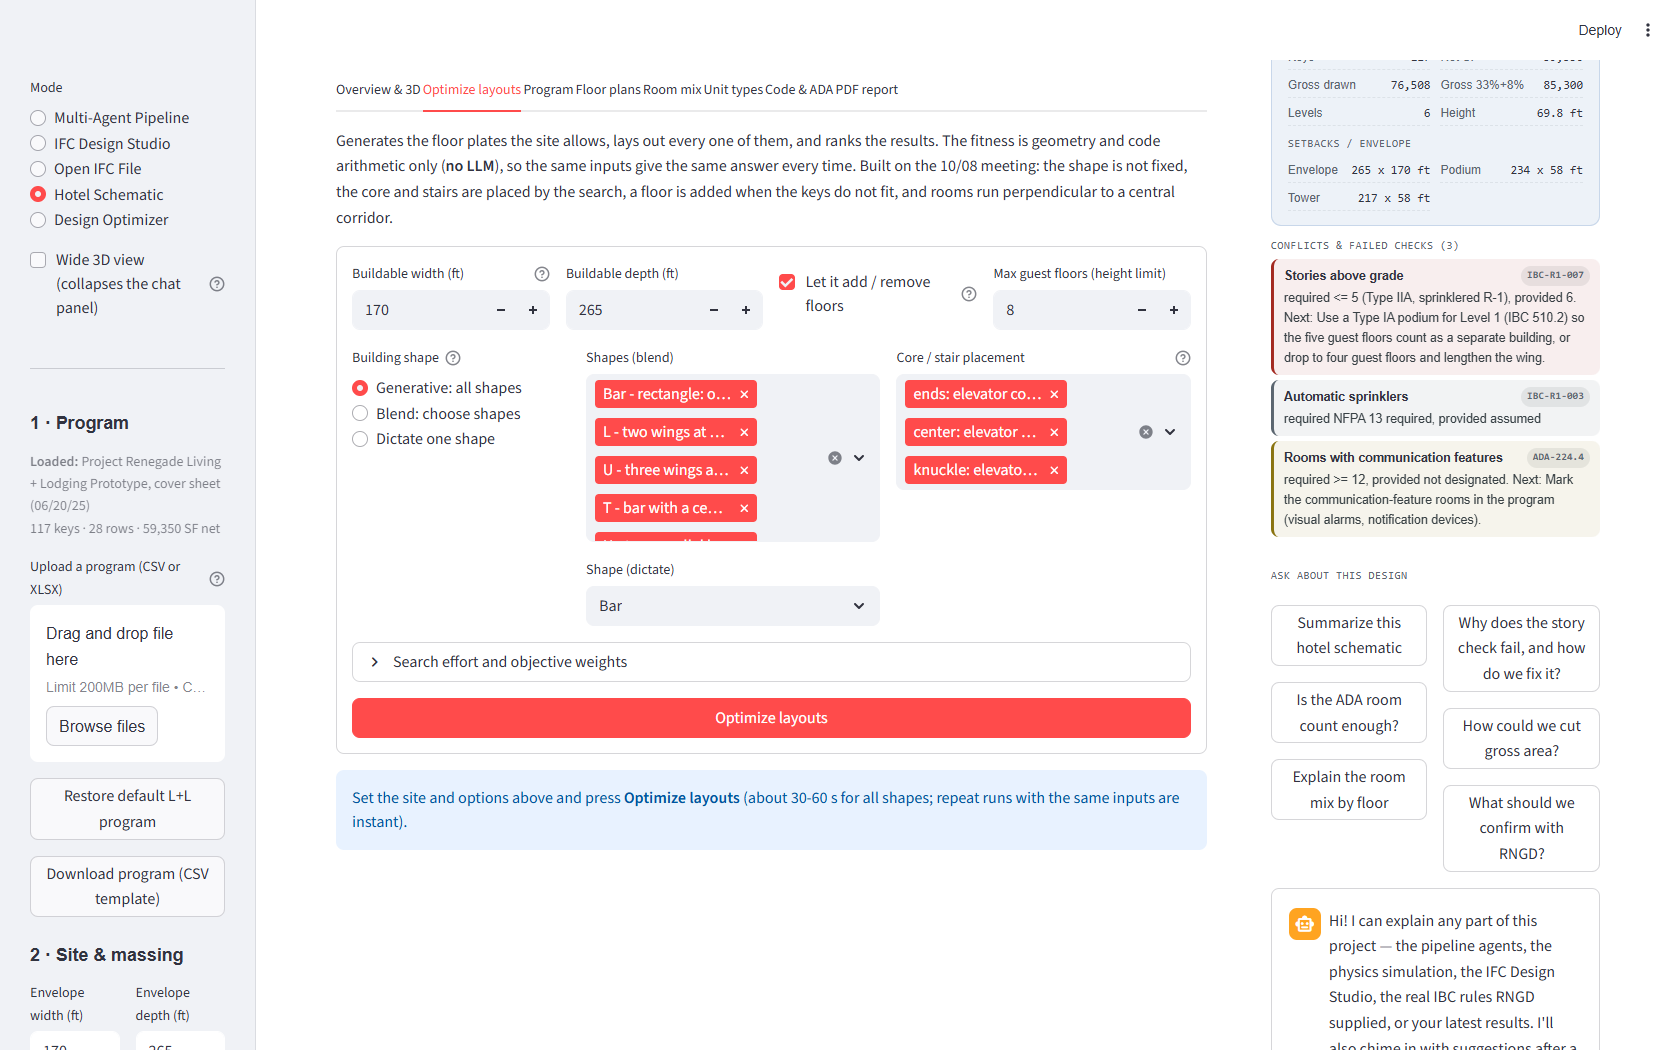
\includegraphics[width=\linewidth,keepaspectratio,height=0.42\textheight]{screens/32_hotel_optimize_settings.png}\caption{Optimize layouts: buildable area, shape mode (generative, blend or one shape), core placement and floors.}\end{figure}
\begin{figure}[H]\centering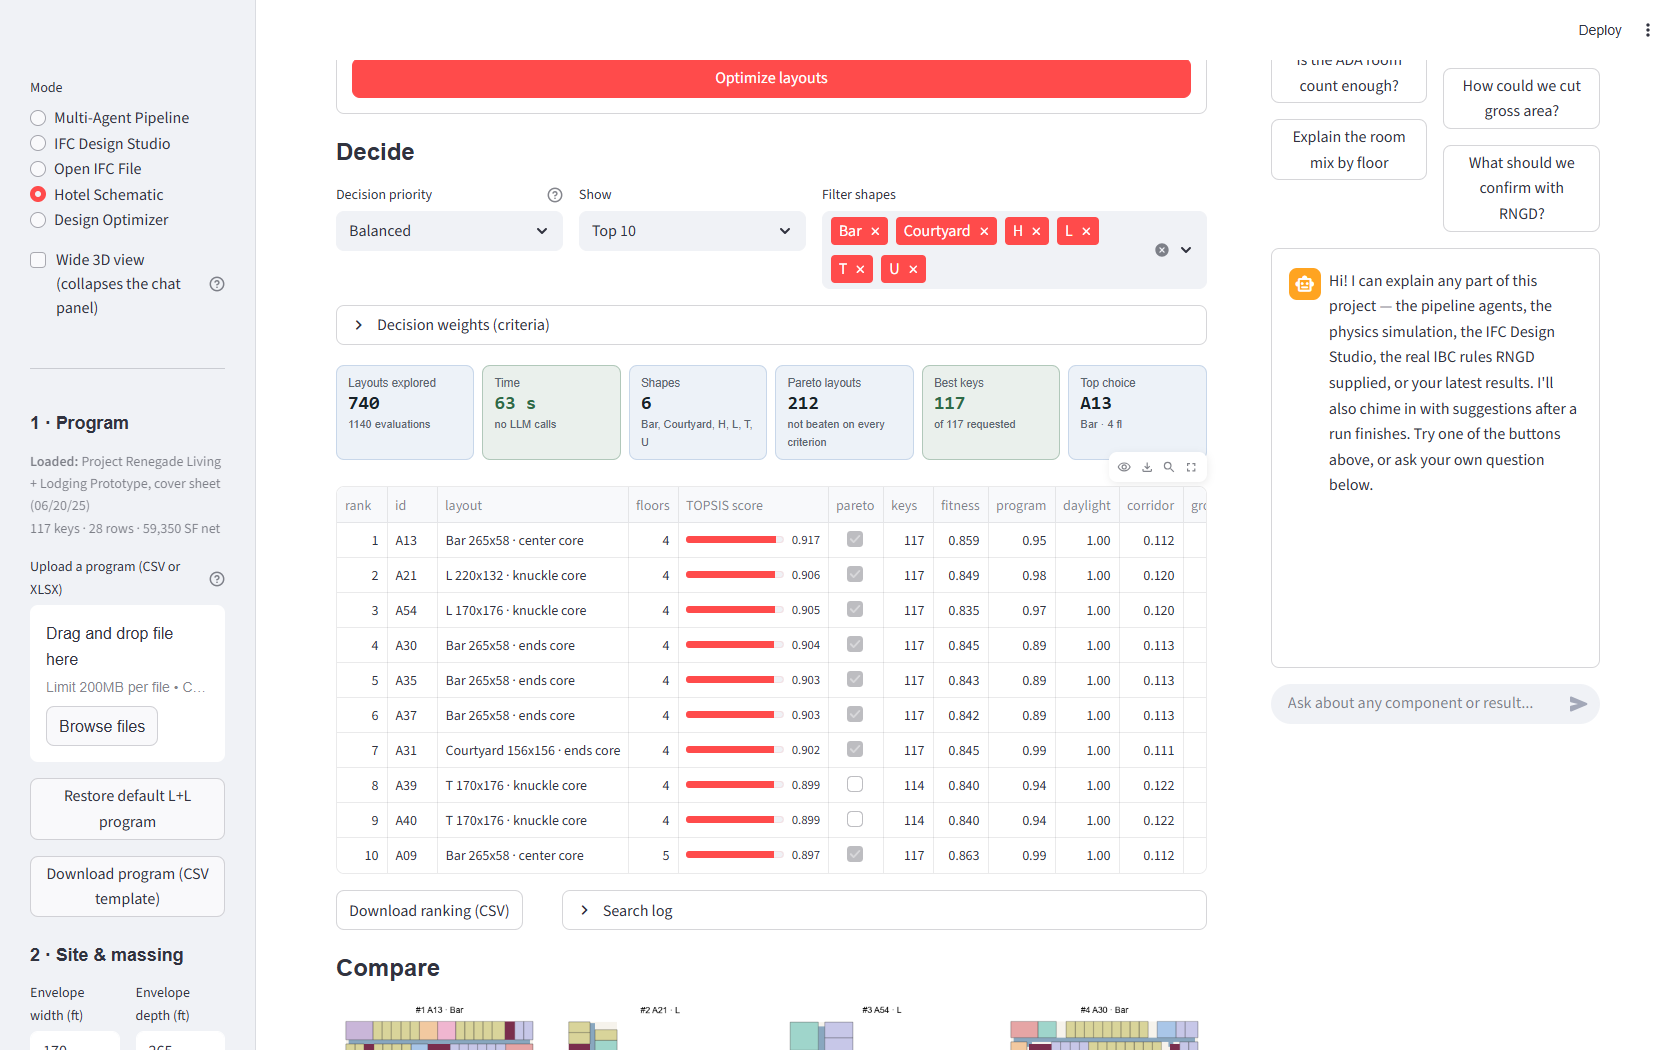
\includegraphics[width=\linewidth,keepaspectratio,height=0.42\textheight]{screens/33_hotel_optimize_decide.png}\caption{Decision step: every distinct layout ranked by TOPSIS under the chosen priority, with the Pareto flag; the Show dropdown switches between the top 5, 10 or 25, the Pareto front and all layouts.}\end{figure}
\begin{figure}[H]\centering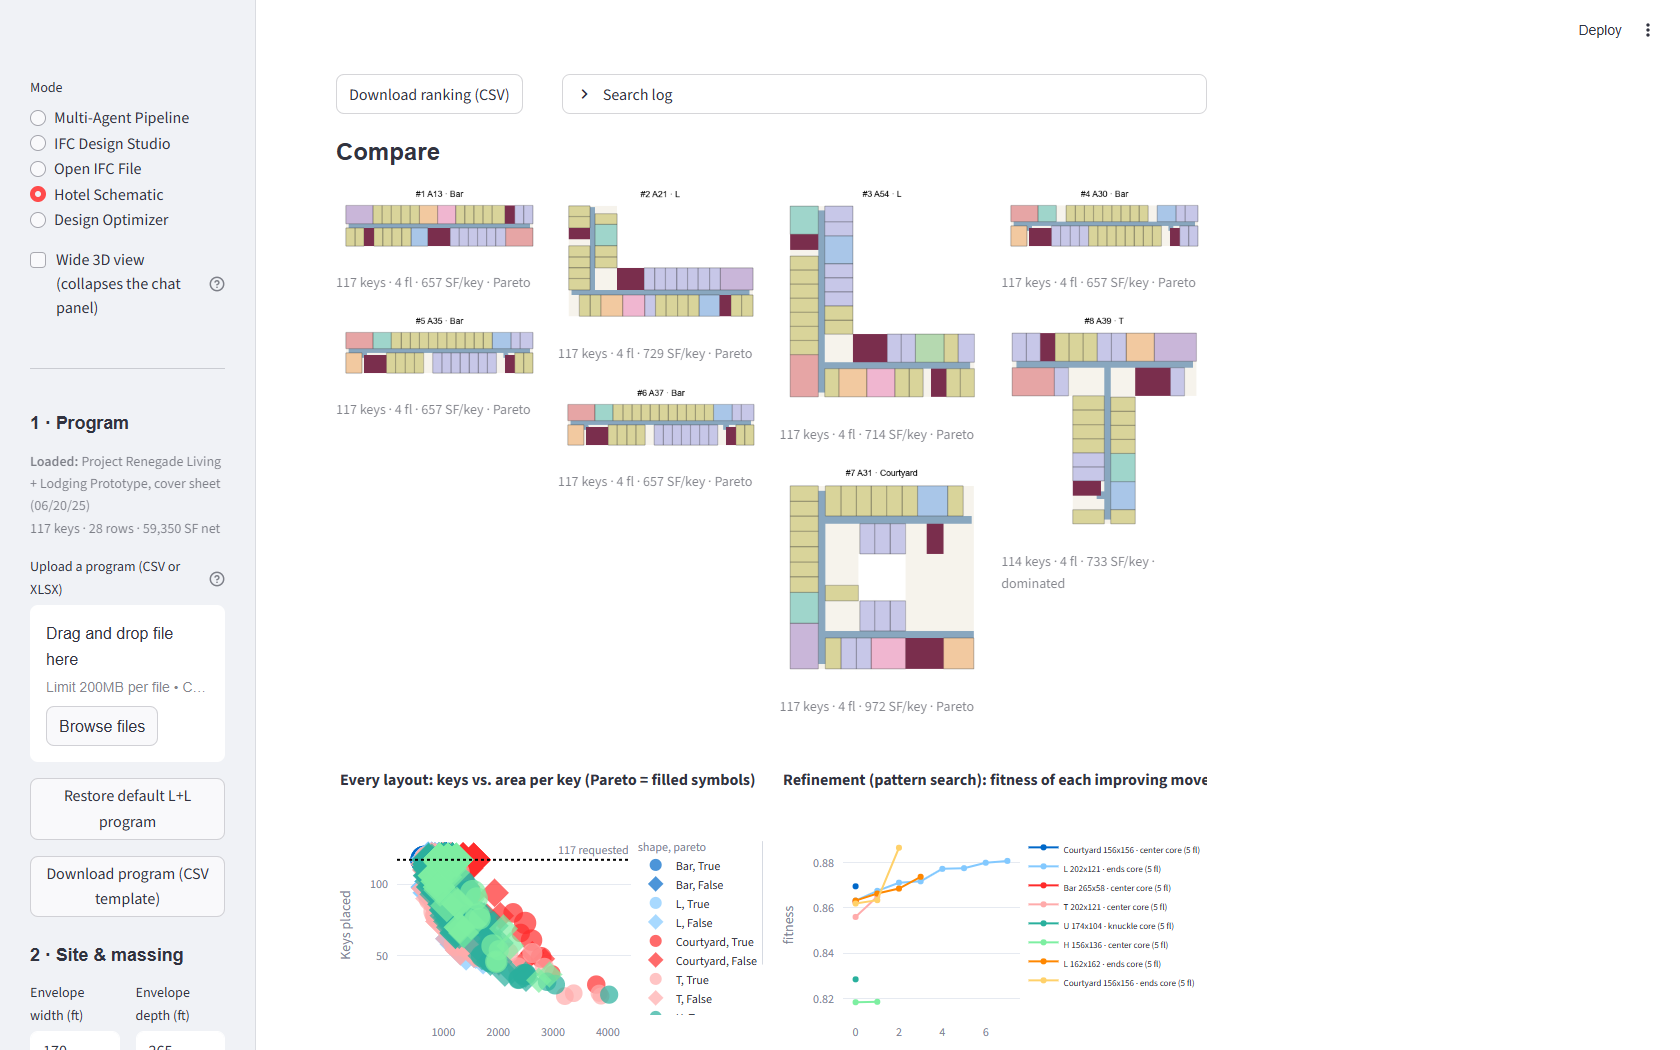
\includegraphics[width=\linewidth,keepaspectratio,height=0.42\textheight]{screens/34_hotel_optimize_compare.png}\caption{Comparison: typical-floor thumbnails of the first-ranked layouts, keys against gross area per key for every layout, and the fitness gained by pattern search.}\end{figure}
\begin{figure}[H]\centering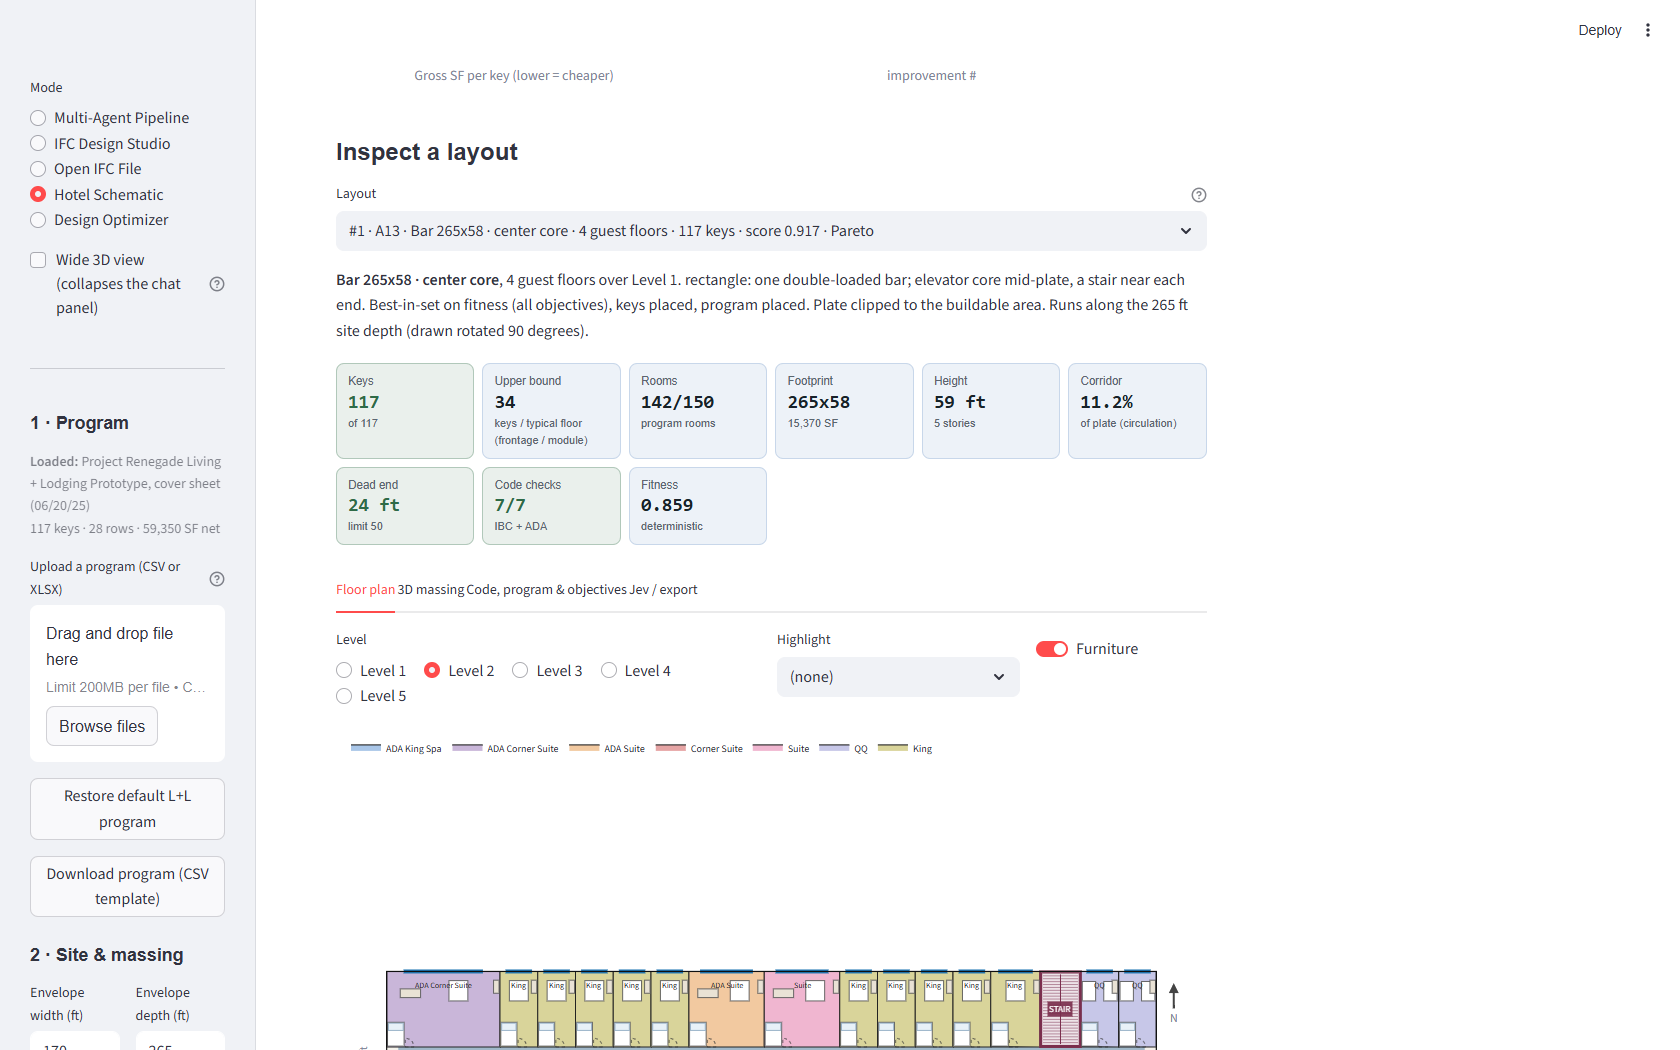
\includegraphics[width=\linewidth,keepaspectratio,height=0.42\textheight]{screens/35_hotel_optimize_inspect.png}\caption{One layout inspected: keys, upper bound, footprint, corridor share, dead end, code checks and fitness.}\end{figure}
\begin{figure}[H]\centering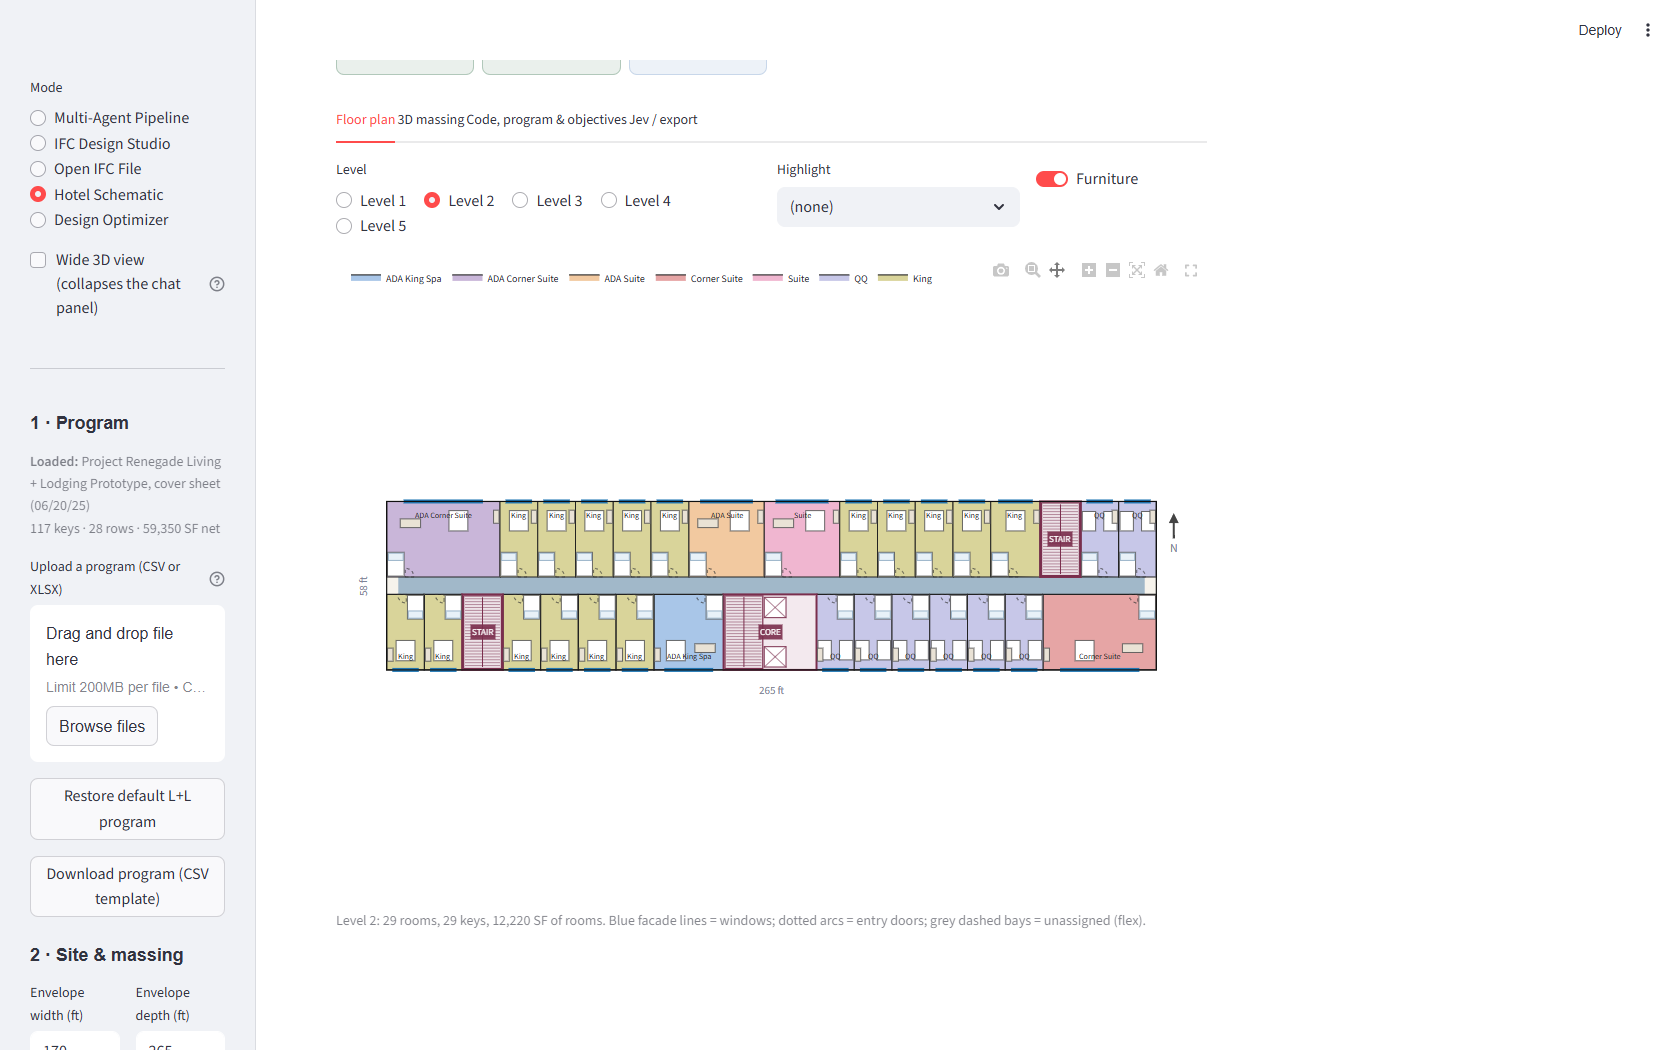
\includegraphics[width=\linewidth,keepaspectratio,height=0.42\textheight]{screens/36_hotel_optimize_plan.png}\caption{Interactive furnished plan of the selected layout (hover gives room data).}\end{figure}
\begin{figure}[H]\centering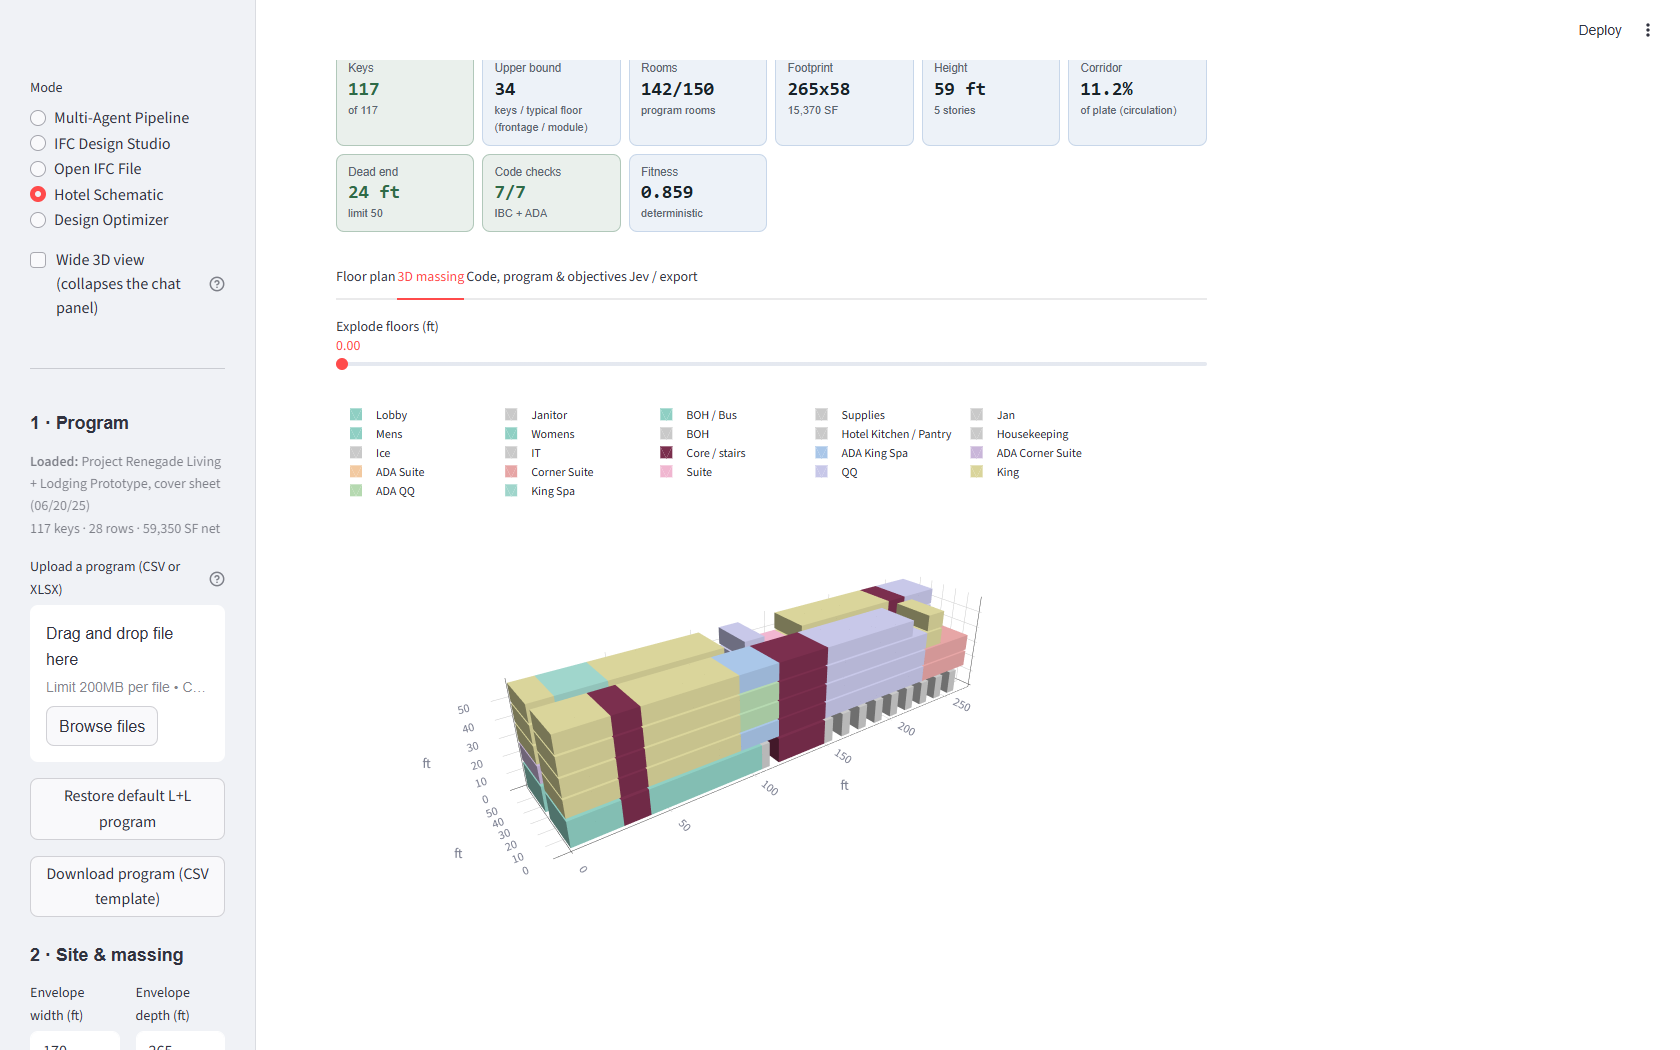
\includegraphics[width=\linewidth,keepaspectratio,height=0.42\textheight]{screens/37_hotel_optimize_3d.png}\caption{Stacked 3D massing of the selected layout, coloured by room type.}\end{figure}

\subsection{What is still open}
\begin{itemize}
\item Level 1 uses the same plate as the guest floors (no wider podium), so large ground-floor rooms can be left out; they are listed for every layout.
\item The decoder draws rectangles on a 1 ft grid: angled wings, curved facades and structural grids are not modelled.
\item The upper bounds are loose; a tight bound would need an exact packing model.
\item The centre-core scheme uses two stairs; on T, U and H plates the third wing can exceed the dead-end limit. The check flags it and the ranking moves such layouts down.
\item Parking, cost and energy are not in the fitness. Facade length per key and gross area per key stand in for cost in the decision step.
\item Jev (TypeSafe's hosted decision model) is wired only as an optional advisor; no key was configured for this run.
\end{itemize}


\section{Assistant}
The chat panel answers with the live state of whichever mode is open (pipeline result, IFC design, real IFC summary,
hotel schematic) plus retrieved passages from the knowledge base and RNGD's documents.

\textbf{Question (one-click button):} Why does the story check fail, and how do we fix it?

\textbf{Answer, as given in the run} (reproduced verbatim; LLM answers are not fact-checked and can misstate code details --- the code screen in Section~\ref{sec:hotel} is the authoritative result):\par
\begin{quote}Why the story-count check fails\par
{\footnotesize\begin{longtable}{p{3.75cm}p{3.75cm}p{3.75cm}p{3.75cm}}\toprule
\textbf{Rule} & \textbf{Requirement} & \textbf{What the model shows} & \textbf{Why it fails} \\ \midrule
IBC-R1-007 – Stories above grade (RNGD’s real 2021 IBC CSV) & $\le$ 5 stories above the grade plane for a sprinklered R-1, Type IIA building & 6 stories above grade (Level 1 podium + 5 guest floors) & The podium is being counted as a “story above grade” because it is a finished, occupiable floor (lobby/BOH). The IBC treats any occupiable floor that meets the definition of a story (height $\ge$ 8 ft, has a ceiling, is not a mezzanine) as part of the story count. With the podium included, the total exceeds the 5-story limit. \\
\bottomrule\end{longtable}}
How to bring the design into compliance\par
Re-classify the podium\par
If the podium can be treated as a non-habitable “parking/mechanical” level (Type IA, not Type IIA), the IBC allows it to be excluded from the “stories above grade” count.\par
Change the podium program from Lobby + BOH to a parking/garage or service level that is not occupied (no sleeping rooms, no assembly).\par
Update the code-screen to mark the podium as “non-habitable”; the story count will then be 5 (guest floors only) and the rule will PASS.\par
Reduce the number of guest floors\par
Drop one guest floor (e.g., go from 5 guest floors to 4).\par
Keep the podium as a regular lobby/BOH (still counted) → total stories = 5 → PASS.\par
This will lower total GSF and may affect unit count; you’ll need to re-run the BaaP matching to see if the 117-key program still fits.\par
Apply for a zoning/IBC variance\par
If the client insists on keeping the podium as an occupied floor and the 5-story limit, a variance from the local building authority can be requested.\par
Document the rationale (e.g., podium provides essential public amenities, no additional fire-risk, meets fire-rating requirements).\par
Note: The variance is a non-technical fix; the pipeline will still flag the rule as FAIL until the variance is granted.\par
Combine (1) + (2) for flexibility\par
Convert the podium to a parking/garage level (non-habitable) and keep 5 guest floors.\par
This satisfies the story count and may help the parking shortfall (see the earlier “parking-shortfall” issue).\par
What to do next in the tool\par
Edit the hotel schematic (in the “Hotel Schematic” UI) → change the Level 1 program type or delete one guest floor.\par
Re-run the “Code screen” (the real-IBC check tab) to verify that IBC-R1-007 now PASSes.\par
If you keep the podium as a lobby, run the IFC Design Studio with a structured-parking garage under the podium; that may also solve the separate parking-stall shortfall.\par
Bottom line: The failure is purely a code-count issue—reduce the counted stories or re-classify the podium so it no longer counts as an “above-grade” story. Once that is done, the story-count rule will pass, and you can focus on the remaining parking conflict.\par\end{quote}
\begin{figure}[H]\centering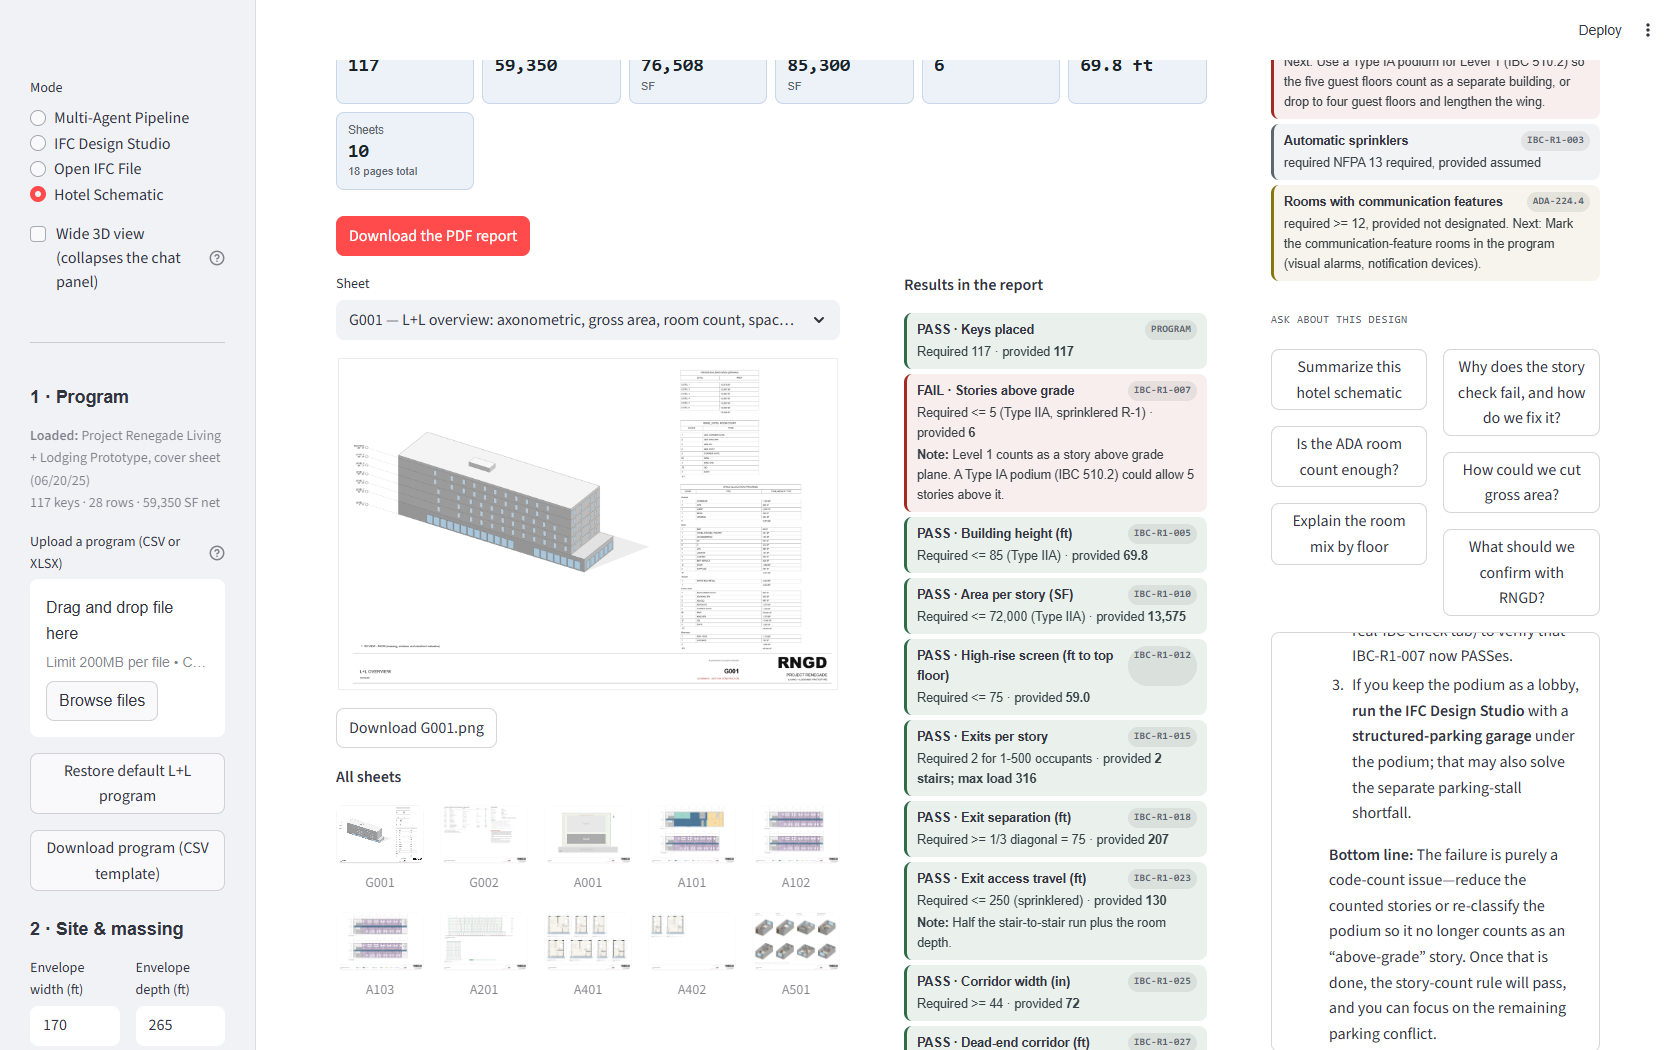
\includegraphics[width=\linewidth,keepaspectratio,height=0.42\textheight]{screens/31_assistant_answer.png}\caption{The assistant answering a one-click question about the hotel design, using the live design state.}\end{figure}


\section{Verification: automated tests}
The full pytest suite was run as part of building this report: 51 of 51 tests passed
(51 passed (results of the last full run, pytest\_results.xml)). App tests drive the real Streamlit app through Streamlit's AppTest, including a full pipeline
run with real LLM calls.
{\small \begin{longtable}{p{2.6cm}p{9.6cm}p{1.0cm}p{1.4cm}}
\toprule
\textbf{File} & \textbf{Test} & \textbf{s} & \textbf{Result} \\ \midrule \endhead
test\_app & test\_loads\_without\_exception\_default\_mode & 28.2 & \textcolor{pass}{\textbf{PASS}} \\
test\_app & test\_ifc\_studio\_scenario\_button\_generates\_design & 4.4 & \textcolor{pass}{\textbf{PASS}} \\
test\_app & test\_ifc\_studio\_shows\_real\_ibc\_tab\_and\_summary\_card & 1.6 & \textcolor{pass}{\textbf{PASS}} \\
test\_app & test\_quick\_question\_button\_asks\_and\_replies & 32.6 & \textcolor{pass}{\textbf{PASS}} \\
test\_app & test\_real\_docs\_loaded\_into\_knowledge\_base & 0.1 & \textcolor{pass}{\textbf{PASS}} \\
test\_app & test\_chat\_panel\_replies & 20.2 & \textcolor{pass}{\textbf{PASS}} \\
test\_app & test\_open\_ifc\_file\_explorer & 9.4 & \textcolor{pass}{\textbf{PASS}} \\
test\_app & test\_full\_pipeline\_run\_via\_ui & 52.2 & \textcolor{pass}{\textbf{PASS}} \\
test\_app & test\_hotel\_mode\_tabs\_and\_controls & 6.7 & \textcolor{pass}{\textbf{PASS}} \\
test\_app & test\_hotel\_optimize\_layouts\_tab & 13.4 & \textcolor{pass}{\textbf{PASS}} \\
test\_app & test\_design\_optimizer\_mode\_runs\_and\_exports\_pdf & 5.6 & \textcolor{pass}{\textbf{PASS}} \\
test\_hotel & test\_default\_program\_totals & 0.0 & \textcolor{pass}{\textbf{PASS}} \\
test\_hotel & test\_net\_to\_gross\_rounds\_up\_to\_hundred & 0.0 & \textcolor{pass}{\textbf{PASS}} \\
test\_hotel & test\_schematic\_places\_all\_keys & 0.0 & \textcolor{pass}{\textbf{PASS}} \\
test\_hotel & test\_six\_levels\_flagged\_against\_five\_story\_rule & 0.0 & \textcolor{pass}{\textbf{PASS}} \\
test\_hotel & test\_upload\_csv & 0.0 & \textcolor{pass}{\textbf{PASS}} \\
test\_hotel & test\_detailed\_program\_matches\_source\_schedule & 0.0 & \textcolor{pass}{\textbf{PASS}} \\
test\_hotel & test\_stairs\_and\_core\_stack\_on\_every\_level & 0.0 & \textcolor{pass}{\textbf{PASS}} \\
test\_hotel & test\_per\_floor\_support\_rooms\_on\_each\_guest\_floor & 0.0 & \textcolor{pass}{\textbf{PASS}} \\
test\_hotel & test\_two\_end\_stairs\_clear\_dead\_end\_and\_fit\_envelope & 0.0 & \textcolor{pass}{\textbf{PASS}} \\
test\_hotel & test\_ground\_floor\_places\_every\_non\_guest\_row & 0.0 & \textcolor{pass}{\textbf{PASS}} \\
test\_hotel & test\_uploaded\_program\_draws\_a\_plan\_sheet & 0.9 & \textcolor{pass}{\textbf{PASS}} \\
test\_hotel & test\_ada\_tables\_match\_2010\_standards & 0.0 & \textcolor{pass}{\textbf{PASS}} \\
test\_hotel & test\_program\_detail\_and\_mix\_by\_floor & 0.0 & \textcolor{pass}{\textbf{PASS}} \\
test\_hotel & test\_per\_floor\_rooms\_follow\_floor\_count & 0.0 & \textcolor{pass}{\textbf{PASS}} \\
test\_hotel & test\_interactive\_figures\_build & 0.1 & \textcolor{pass}{\textbf{PASS}} \\
test\_hotel\_optimize & test\_plates\_fit\_envelope\_and\_have\_cores & 0.3 & \textcolor{pass}{\textbf{PASS}} \\
test\_hotel\_optimize & test\_elevators\_follow\_keys & 0.0 & \textcolor{pass}{\textbf{PASS}} \\
test\_hotel\_optimize & test\_explore\_is\_deterministic\_and\_places\_the\_keys & 4.8 & \textcolor{pass}{\textbf{PASS}} \\
test\_hotel\_optimize & test\_decision\_ranking\_pareto\_and\_topsis & 2.6 & \textcolor{pass}{\textbf{PASS}} \\
test\_ifc\_design & test\_module\_counts\_sum\_to\_units & 0.0 & \textcolor{pass}{\textbf{PASS}} \\
test\_ifc\_design & test\_compliant\_scenario\_passes\_all\_checks & 0.0 & \textcolor{pass}{\textbf{PASS}} \\
test\_ifc\_design & test\_baseline\_reports\_parking\_shortfall & 0.0 & \textcolor{pass}{\textbf{PASS}} \\
test\_ifc\_design & test\_higher\_floor\_count\_shrinks\_footprint & 0.0 & \textcolor{pass}{\textbf{PASS}} \\
test\_ifc\_design & test\_zoning\_preset\_changes\_limits & 0.0 & \textcolor{pass}{\textbf{PASS}} \\
test\_ifc\_design & test\_accessible\_units\_present & 0.0 & \textcolor{pass}{\textbf{PASS}} \\
test\_ifc\_design & test\_ifc\_roundtrip[Baseline: 4 floors, surface parking] & 1.5 & \textcolor{pass}{\textbf{PASS}} \\
test\_ifc\_design & test\_ifc\_roundtrip[Right-sized: 60 units, podium (compliant)] & 0.8 & \textcolor{pass}{\textbf{PASS}} \\
test\_ifc\_design & test\_ifc\_roundtrip[Podium parking, 5 floors] & 1.5 & \textcolor{pass}{\textbf{PASS}} \\
test\_ifc\_design & test\_ifc\_roundtrip[Dense R-6, 7 floors + podium] & 1.4 & \textcolor{pass}{\textbf{PASS}} \\
test\_ifc\_design & test\_ifc\_roundtrip[Suburban R-2, 60 units, 3 floors] & 0.8 & \textcolor{pass}{\textbf{PASS}} \\
test\_optimizer & test\_site\_and\_programs\_load & 0.0 & \textcolor{pass}{\textbf{PASS}} \\
test\_optimizer & test\_reference\_designs\_reconstruct\_exactly[1-982] & 0.0 & \textcolor{pass}{\textbf{PASS}} \\
test\_optimizer & test\_reference\_designs\_reconstruct\_exactly[2-737] & 0.0 & \textcolor{pass}{\textbf{PASS}} \\
test\_optimizer & test\_reference\_designs\_reconstruct\_exactly[3-913] & 0.0 & \textcolor{pass}{\textbf{PASS}} \\
test\_optimizer & test\_decoder\_is\_valid\_and\_deterministic & 0.1 & \textcolor{pass}{\textbf{PASS}} \\
test\_optimizer & test\_search\_improves\_and\_exports & 1.1 & \textcolor{pass}{\textbf{PASS}} \\
test\_optimizer & test\_heuristic\_review\_and\_weight\_tuning & 0.0 & \textcolor{pass}{\textbf{PASS}} \\
test\_optimizer & test\_fact\_check\_flags\_invented\_numbers & 0.0 & \textcolor{pass}{\textbf{PASS}} \\
test\_optimizer & test\_layout\_quality\_on\_reference\_program & 0.2 & \textcolor{pass}{\textbf{PASS}} \\
test\_optimizer & test\_systematic\_search\_is\_deterministic\_and\_monotonic & 3.0 & \textcolor{pass}{\textbf{PASS}} \\
\bottomrule
\end{longtable}}


\section{Limitations}
\begin{itemize}
\item Pipeline and IFC-studio inputs (customer request, site, zoning presets, BaaP catalog) are synthetic sample data.
\item LLM outputs vary between runs; the pipeline numbers above are from this run only.
\item The hotel layout is a rule-based schematic: parking, structure and MEP are not modelled; fixtures are typical.
\item The optimized layouts are rectangles on a 1 ft grid with one plate for all levels; open items are listed at the end of Section~\ref{sec:opt}.
\item Code screens are planning-level, not code determinations. 3D views are WebGL (app) and painter's-algorithm axonometrics (PDF).
\end{itemize}

\appendix
\section{Screenshot index}
{\small \begin{longtable}{p{4.4cm}p{2.8cm}p{8.8cm}}
\toprule
\textbf{File} & \textbf{Mode} & \textbf{Caption} \\ \midrule \endhead
01\_pipeline\_inputs.png & Multi-Agent Pipeline & Multi-Agent Pipeline before a run: the sample customer request and site sketch that feed the agents; the assistant panel on the right. \\
02\_pipeline\_running.png & Multi-Agent Pipeline & The pipeline running live: each agent reports its step as it finishes. \\
03\_pipeline\_overview.png & Multi-Agent Pipeline & Pipeline result overview: the arbiter's decision, confidence and conflict count. \\
04\_pipeline\_agent\_trace.png & Multi-Agent Pipeline & Agent trace: every agent step with model, status and latency. \\
05\_pipeline\_program\_site.png & Multi-Agent Pipeline & Program parsed from the request and the computed site constraints. \\
06\_pipeline\_baap\_conflicts.png & Multi-Agent Pipeline & BaaP module counts and the conflicts the Conflict Agent found. \\
07\_pipeline\_site\_simulation.png & Multi-Agent Pipeline & Physics-style site simulation and the computer-vision QA of the rendered plan. \\
08\_pipeline\_floor\_plates.png & Multi-Agent Pipeline & Rule-based floor plates (ground and typical floor). \\
09\_pipeline\_final\_decision.png & Multi-Agent Pipeline & The arbiter's final decision, unresolved issues and next steps. \\
10\_ifc\_baseline\_3d\_model.png & IFC Design Studio & IFC Design Studio, Baseline scenario (120 units, 4 floors, surface parking): the generated IFC4 model in the 3D viewer. \\
11\_ifc\_baseline\_site\_plan.png & IFC Design Studio & Baseline site plan: building, parking, easement and fire lane on the synthetic lot. \\
12\_ifc\_baseline\_compliance.png & IFC Design Studio & Baseline compliance against the ten sample-zoning checks. \\
13\_ifc\_baseline\_real\_ibc\_check.png & IFC Design Studio & Baseline cross-checked against RNGD's real 2021 IBC rules. \\
14\_ifc\_baseline\_how\_this\_was\_built.png & IFC Design Studio & Step-by-step explanation of how the layout was generated. \\
15\_ifc\_rightsized\_compliance.png & IFC Design Studio & Right-sized scenario (60 units, podium parking): the compliance checks after the fix. \\
16\_ifc\_rightsized\_3d.png & IFC Design Studio & Right-sized scenario in 3D. \\
17\_explorer\_3d\_model.png & Open IFC File & A real IFC file (CDI Solutions, Metairie Bank, IFC2X3, 89 MB) recentred and shown in 3D. \\
18\_explorer\_summary.png & Open IFC File & What is in the real model: schema, storeys and element counts by IFC class. \\
19\_explorer\_element\_browser.png & Open IFC File & Searchable list of the model's elements. \\
20\_hotel\_overview.png & Hotel Schematic & Hotel Schematic workspace: KPI tiles, the room-by-room 3D model and the key results with suggested fixes. \\
21\_hotel\_program.png & Hotel Schematic & The editable program (Project Renegade L+L space allocation, 28 rows) with area and room-mix charts. \\
22\_hotel\_floor.png & Hotel Schematic & Interactive floor plan of Level 1 (hover shows each room's area and size). \\
23\_hotel\_program\_detail.png & Hotel Schematic & Detailed program: per-room size, beds, sleeping capacity, placement, IBC occupant load and fit-out. \\
24\_hotel\_plan\_level2.png & Hotel Schematic & Interactive plan of Level 2, a typical guest floor (24 keys). \\
25\_hotel\_plan\_drawing.png & Hotel Schematic & The same level in drawing style (as used on the PDF sheets). \\
26\_hotel\_room.png & Hotel Schematic & Keys of each room type on each guest floor. \\
27\_hotel\_unit.png & Hotel Schematic & Unit type detail: enlarged plan and two 3D interior views. \\
28\_hotel\_code.png & Hotel Schematic & Code screen against RNGD's IBC rule set and the 2010 ADA guest-room tables, with rule text. \\
29\_hotel\_report\_results.png & Hotel Schematic & PDF report tab after generating: summary numbers and the results that went into the report. \\
30\_hotel\_report\_sheets.png & Hotel Schematic & Sheet gallery of the generated drawing set. \\
31\_assistant\_answer.png & Assistant & The assistant answering a one-click question about the hotel design, using the live design state. \\
\bottomrule
\end{longtable}}

\end{document}
